All physics objects are reconstructed offline using a particle-flow (PF) algorithm~\cite{CMS:particle_flow}.
The aim of the algorithm is to reconstruct all final-state particles (photons, charged and neutral hadrons, muons, and electrons) in the event, using combined information from the CMS detector.
The reconstructed vertex with the largest sum of object $\PT^2$ is taken to be the primary \pp interaction vertex.

Electron candidates are identified using the combination of the silicon tracker and the corresponding ECAL cluster information~\cite{CMS:el_PF}.
Electron energies are determined using the momenta derived from the electron track in the tracker system, the energy of the spatially compatible ECAL cluster, and the sum of all compatible bremsstrahlung photon energies.
In order to reject events with misidentified electron candidates and candidates originating from photon conversions, additional electron identification requirements are applied.
A PF-based combined relative isolation, \Irel, is defined as the \PT sum of all neutral hadron, charged hadron, and photon candidates within a cone of size $\DR = \sqrt{\smash[b]{(\Delta\eta)^2+(\Delta\phi)^2}} < 0.4$ (where $\phi$ is the azimuthal angle in radians) around the lepton direction, divided by the lepton \PT, with a correction to suppress the residual effect of pileup~\cite{CMS:el_reliso}.
The isolated electron candidate is required to have $\PT>38\GeV$, $\abseta < 2.4$, and $\Irel < 0.0287+0.506/\PT$ ($0.0445+0.963/\PT$) in the barrel (endcaps), with \PT in \GeV.
Due to reduced reconstruction efficiency, the gap ($1.44 < \abseta < 1.57$) between the barrel and endcap parts of the ECAL is excluded.
Events with additional electrons satisfying a looser set of selection criteria with a lower-\PT threshold and a looser isolation requirement are rejected to reduce the background contribution (\eg, from DY production).

Muon candidates are reconstructed using information obtained in the tracker, combined with the muon system~\cite{CMS:mu_PF}.
Identification methods are applied to reject muon candidates that are misidentified or muons that originated from decay-in-flight.
The isolated muon candidate is required to have $\PT > 30\GeV$, $\abseta < 2.4$, and $\Irel < 0.15$.
Events with additional muons satisfying a looser set of selection criteria are rejected as well.

Jets are clustered using the anti-\kt algorithm with a distance parameter of 0.4~\cite{CMS:fastjet, CMS:antikt}.
The jet \ptvec is defined as the vectorial sum of the momenta of all PF candidates in the jet anti-\kt clustering.
Pileup can contribute additional tracks and calorimetric energy depositions to the jet momentum.
To mitigate this effect, tracks identified as originating from pileup vertices are discarded, and an offset correction is applied to correct for remaining contributions from neutral particles from pileup~\cite{CMS:particle_flow}.
Corrections to the jet energy are applied as a function of jet \PT and $\eta$ by studying discrepancies between simulation and data.
At least four jets are required with $\PT > 30\GeV$, $\abseta < 2.4$, and angular separation relative to the selected lepton of $\DR > 0.4$.
Jets are identified as arising from the hadronization of \PQb quarks, denoted as either \PQb-tagged jets or \PQb jets, using the deep-learned combined secondary-vertex algorithm (\DeepCSV).
This combines the information for a given jet from track impact parameters and secondary vertices into a model optimized through a deep neural network.
The selected working point has a signal identification efficiency of 68\%, with a probability to misidentify \PQc quark, and light-flavor quark and gluon jets as \PQb jets of approximately 12 and 1.1\% in \ttbar events, respectively~\cite{CMS:bjet_eff}.

The top quark and antiquark candidates associated with \PW bosons decaying to \qqbar are reconstructed using one of the \PQb-tagged jets and two non-\PQb-tagged jets in the event through a \chisq algorithm that uses the top quark and \PW boson masses as constraints~\cite{CMS:sorting_algo}.
Those candidates are chosen from the combination having the lowest \chisq value, with the \chisq defined as
\begin{linenomath}\begin{equation}
    \chisq = \left(\frac{\mjjb-\Mt}{\sigt}\right)^2 + \left(\frac{\mjj-\MW}{\sigW}\right)^2,
\end{equation}\end{linenomath}
where \mjjb is the invariant mass of the two non-\PQb-tagged jets and the associated \PQb-tagged jet; \Mt and \sigt are the default top quark mass and average top quark invariant mass resolution of 172.5 and 16.3\GeV, respectively; \mjj is the invariant mass of the two non-\PQb-tagged jets; and \MW and \sigW are the default \PW boson mass and average \PW boson invariant mass resolution of 82.9 and 9.5\GeV, respectively~\cite{CPVtop:chi2value}.
The other \PQb-tagged jet associated with the leptonically decaying \PW boson candidate is assigned as being from the hadronization of a bottom quark or antiquark based on the charge sign of the lepton.
The events can be further categorized into three different types: the correct type represents the events with \PQb jets correctly assigned, the misidentified type stands for the events with \PQb jets are swapped, and the mistag type represents the events with one or all of the selected \PQb jets matched to the wrong objects.
Juding from Fig.~\ref{fig:bbsep_rate}, events with higher minimum \chisq are mainly composed of misidentified and mistag types.
The event purity of the correctly assigned \PQb jets can be raised after imposing an upper bound on the minimum \chisq.
An upper bound of 20 on minimum \chisq achieves around $70\%$ event efficiency with $60\%$ correctly assigned \PQb jets as indicated in Fig.~\ref{fig:bbsep_uppercut}.

However, from simulation it is found that when the invariant mass of the combined isolated lepton and associated \PQb-tagged jet (\Mlb) is greater than 150\GeV, the events have a large fraction of incorrect \PQb jet assignments as shown in Fig.~\ref{fig:opt_lept}.
Therefore, from studies of the simulated \ttbar sample, further requirements of $\chisq < 20$ and $\Mlb < 150\GeV$ are imposed.
This improves the fraction of correctly assigned \PQb jets to $\approx$74\%, while keeping $\approx$65\% of the \ttbar events as shown in Figs~\ref{fig:opt_cut}.

After these selection criteria, the purity of the \ttbar events is 95\%, with single top quark production contributing a background of 3\%.
The upper panels in Figs.~\ref{fig:el_obs_dist} and~\ref{fig:mu_obs_dist} show the distributions of the CP observables for the electron and muon channels, respectively.
The middle panels display the ratio of the data to the simulated distributions, which show reasonable agreement within the one-standard-deviation band.
The bottom panels present the ratio of the CEDM to the SM predictions for $\dtG = \pm 3$.
In these figures, the values of the CP observables are divided by \Mtcub to convert the units to \GeVns.
The systematic uncertainties shown in Figs.~\ref{fig:el_obs_dist} and~\ref{fig:mu_obs_dist}, as well as in later figures and tables, include all systematic uncertainties, except for those due to backgrounds.
The latter uncertainty contributes only to the final \Acp measurements instead of the number of signal events and will be discussed in detail in Section~\ref{sec:uncertainty}.
Table~\ref{tab:signal_region_expected_percentage} shows the predicted signal and background contributions to the signal events from simulation for the electron and muon channels.
The fraction of leptonic tau decays in the SM simulated \ttbar samples is about 0.3\% and the contribution is negligible in the final results.
The QCD and \ttbar multijet events are highly suppressed by the selection requirements and provide negligible contributions of around 0.2 and 0.05\%, respectively, to the signal events.
The estimation of the number of misidentified signal events coming from \ttbar decays to dilepton+jets is discussed in Section~\ref{sec:fitresult}.
\begin{figure}[p]
    \centering
    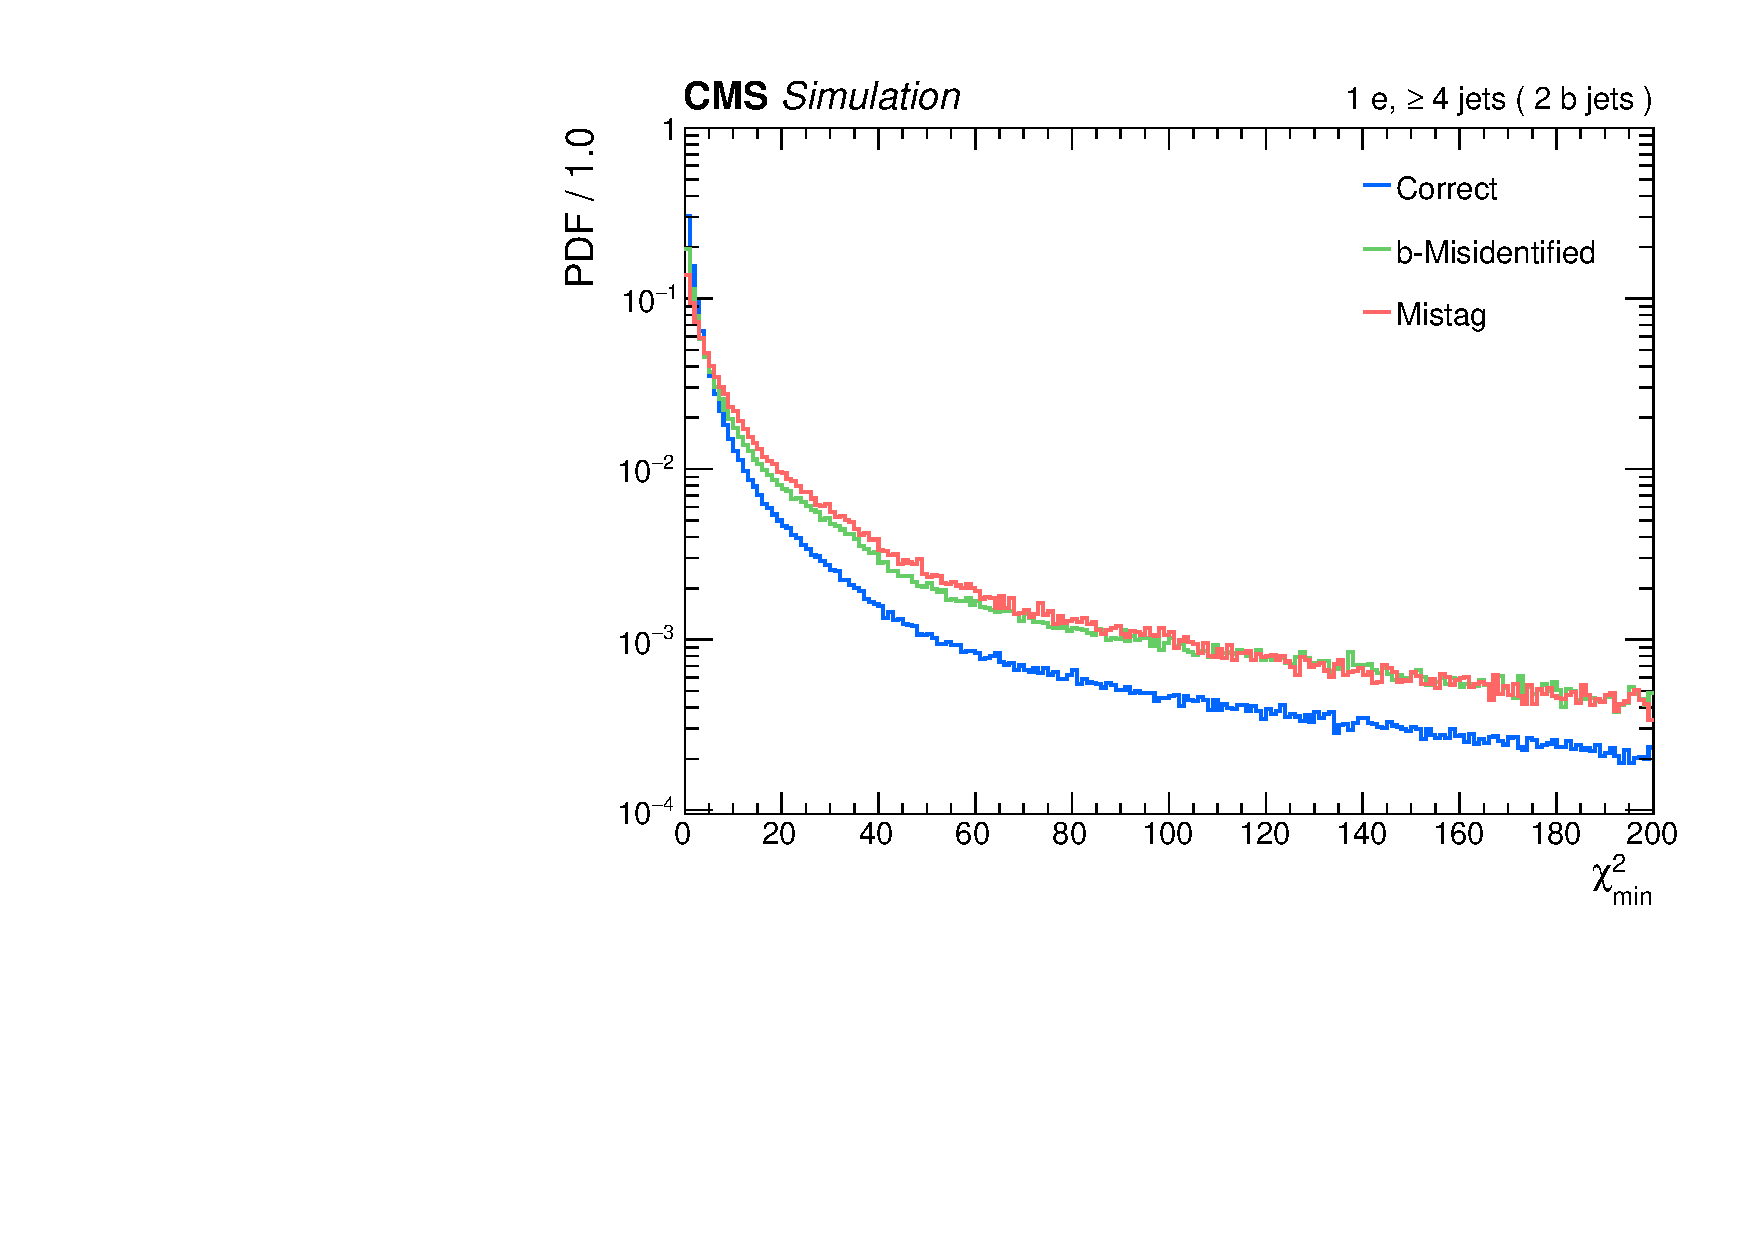
\includegraphics[width=0.45\textwidth]{figure/bbSep_16_el_Rate_PDF_bbSep.pdf}
    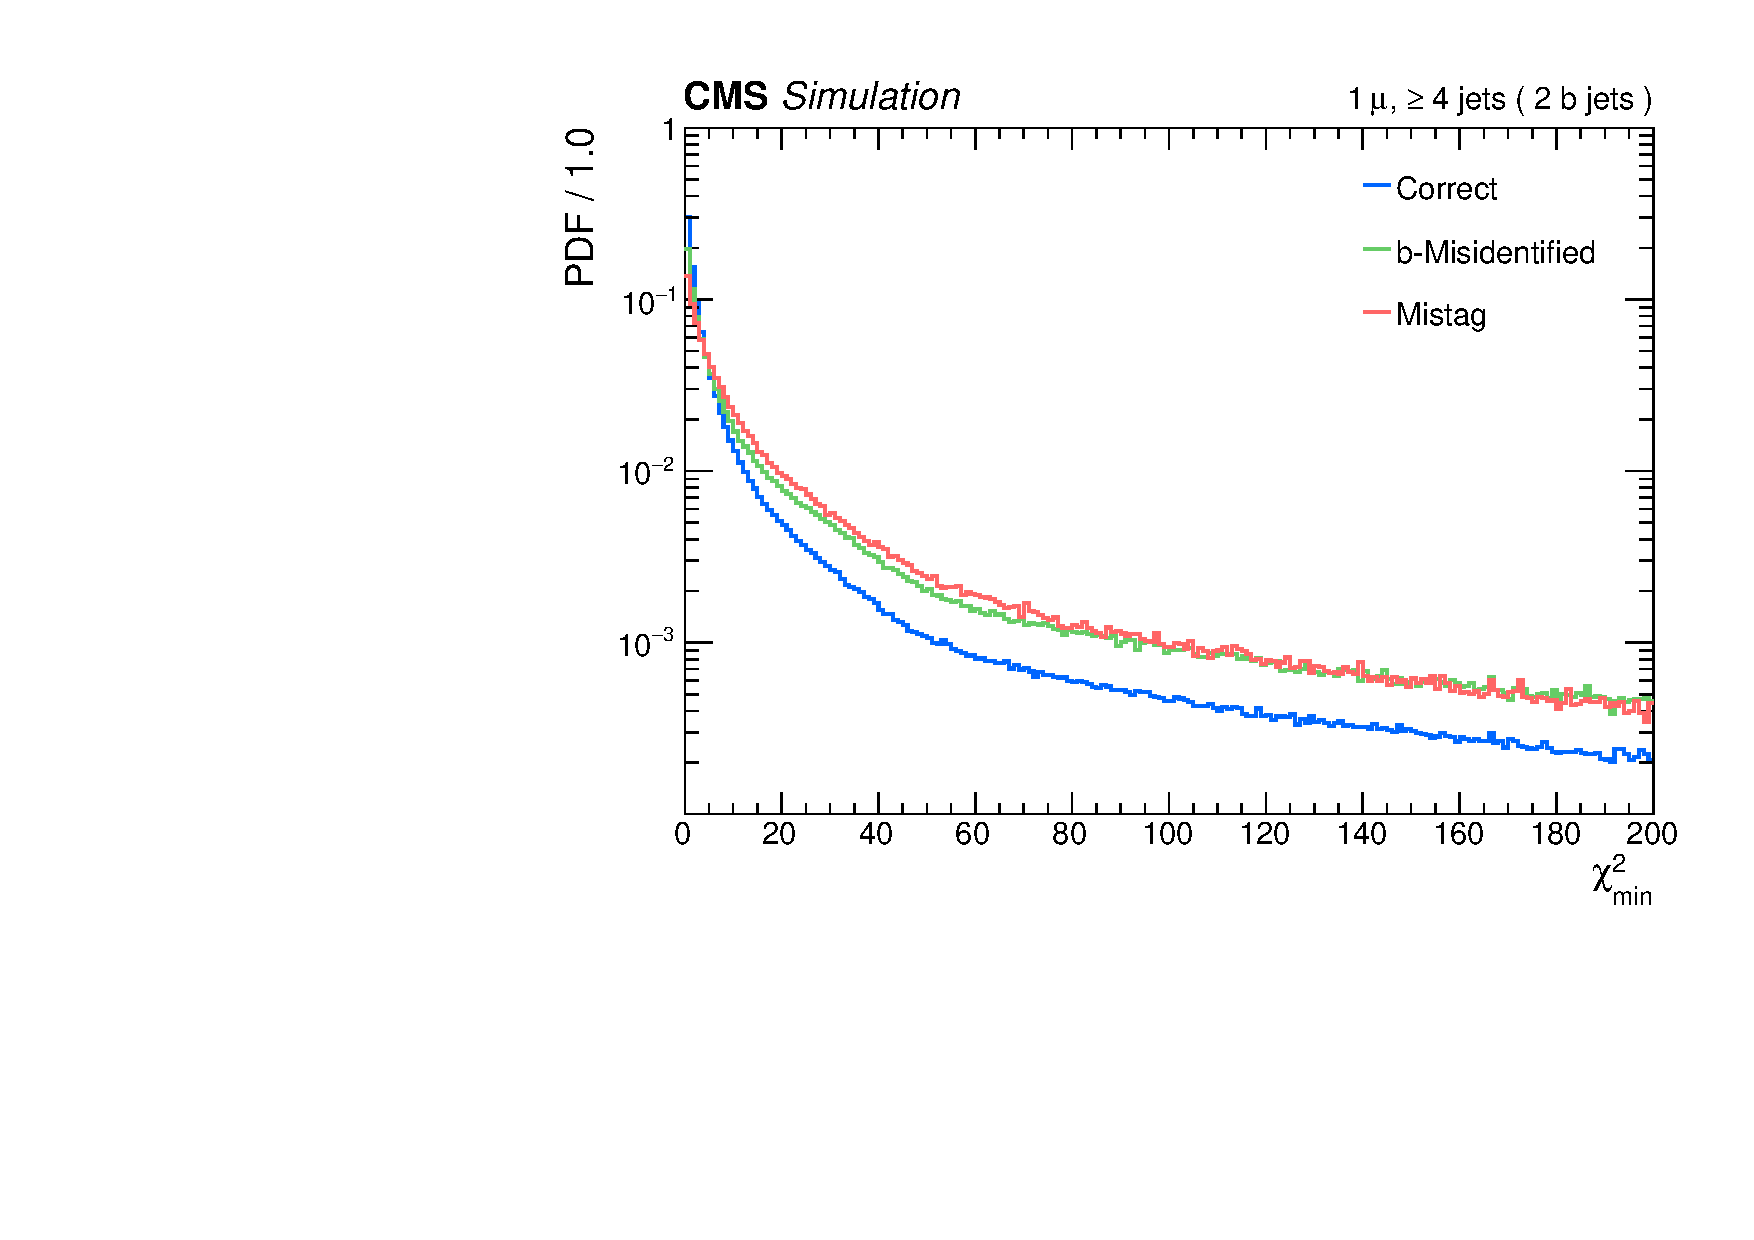
\includegraphics[width=0.45\textwidth]{figure/bbSep_16_mu_Rate_PDF_bbSep.pdf}
    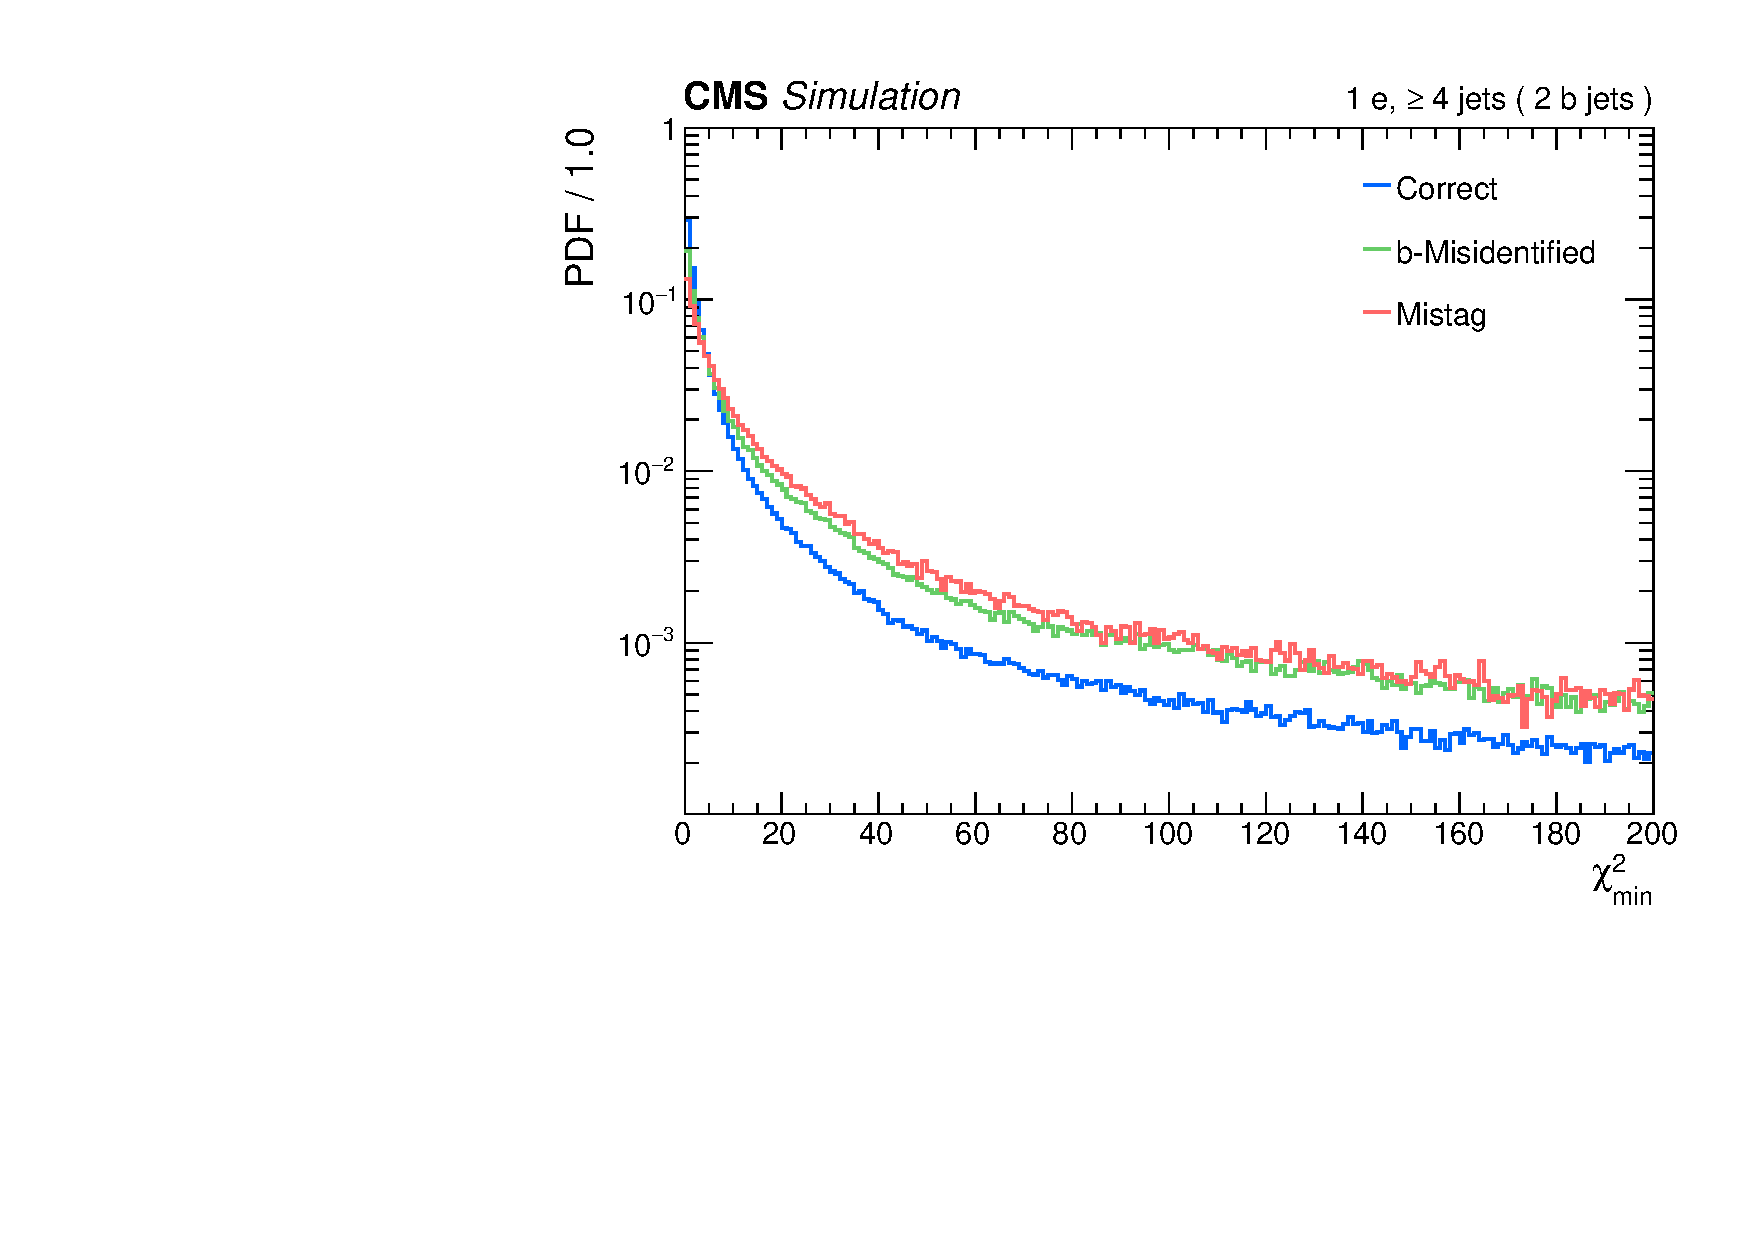
\includegraphics[width=0.45\textwidth]{figure/bbSep_17_el_Rate_PDF_bbSep.pdf}
    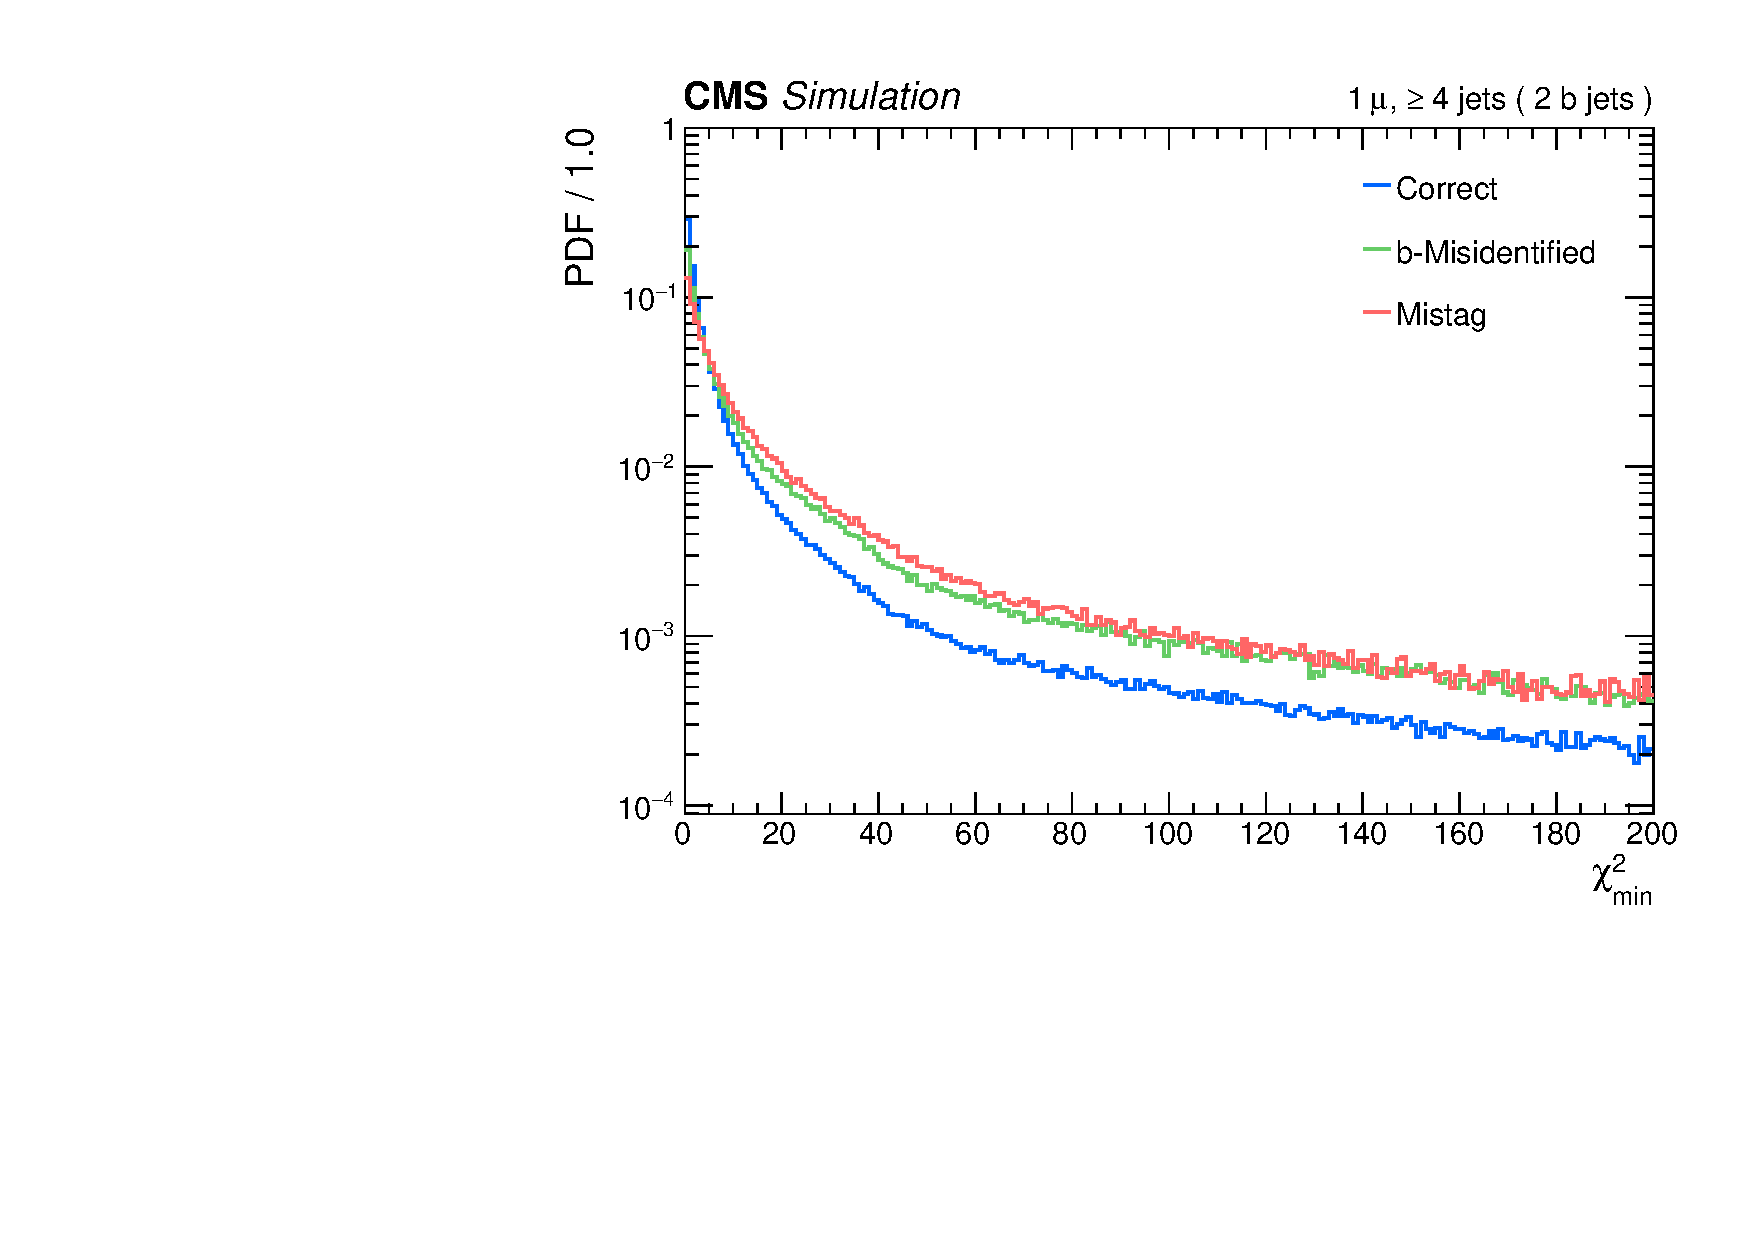
\includegraphics[width=0.45\textwidth]{figure/bbSep_17_mu_Rate_PDF_bbSep.pdf}
    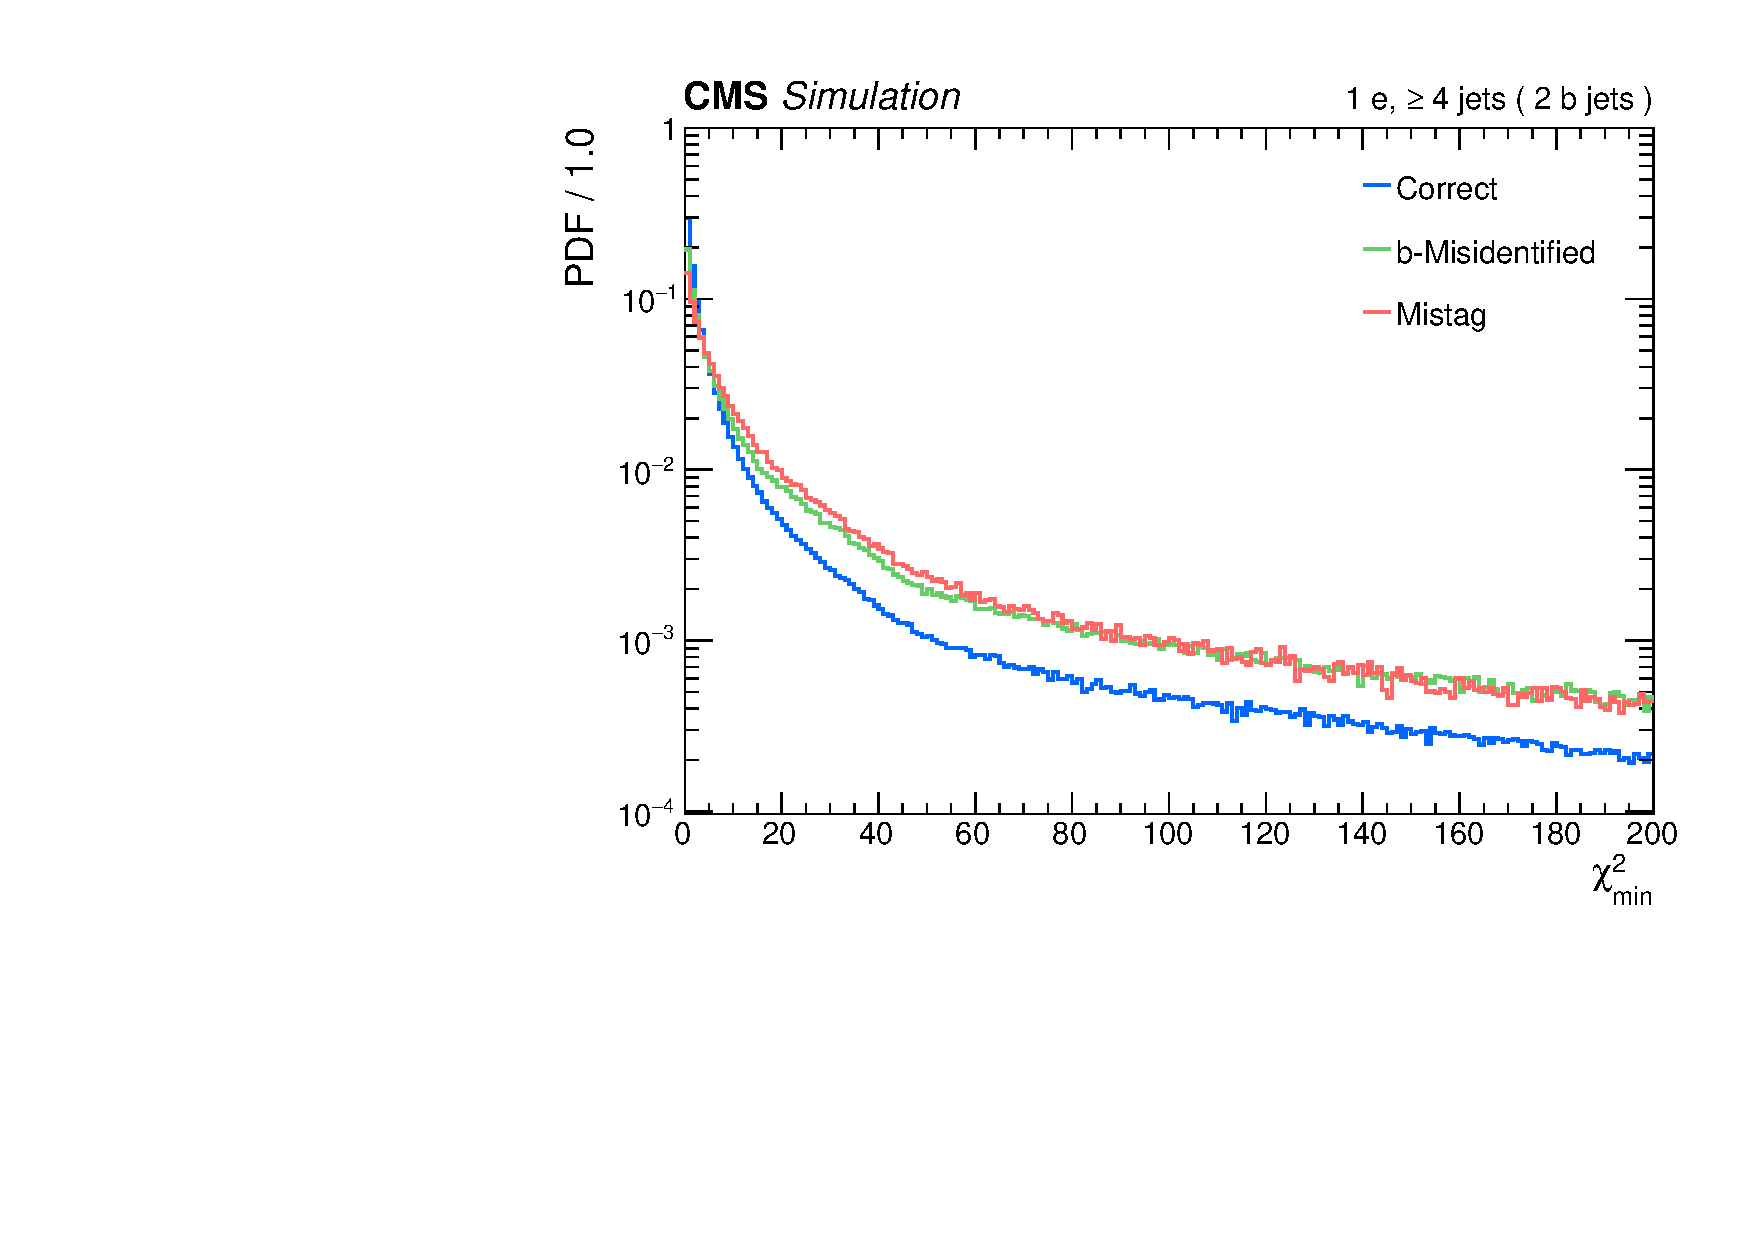
\includegraphics[width=0.45\textwidth]{figure/bbSep_18_el_Rate_PDF_bbSep.pdf}
    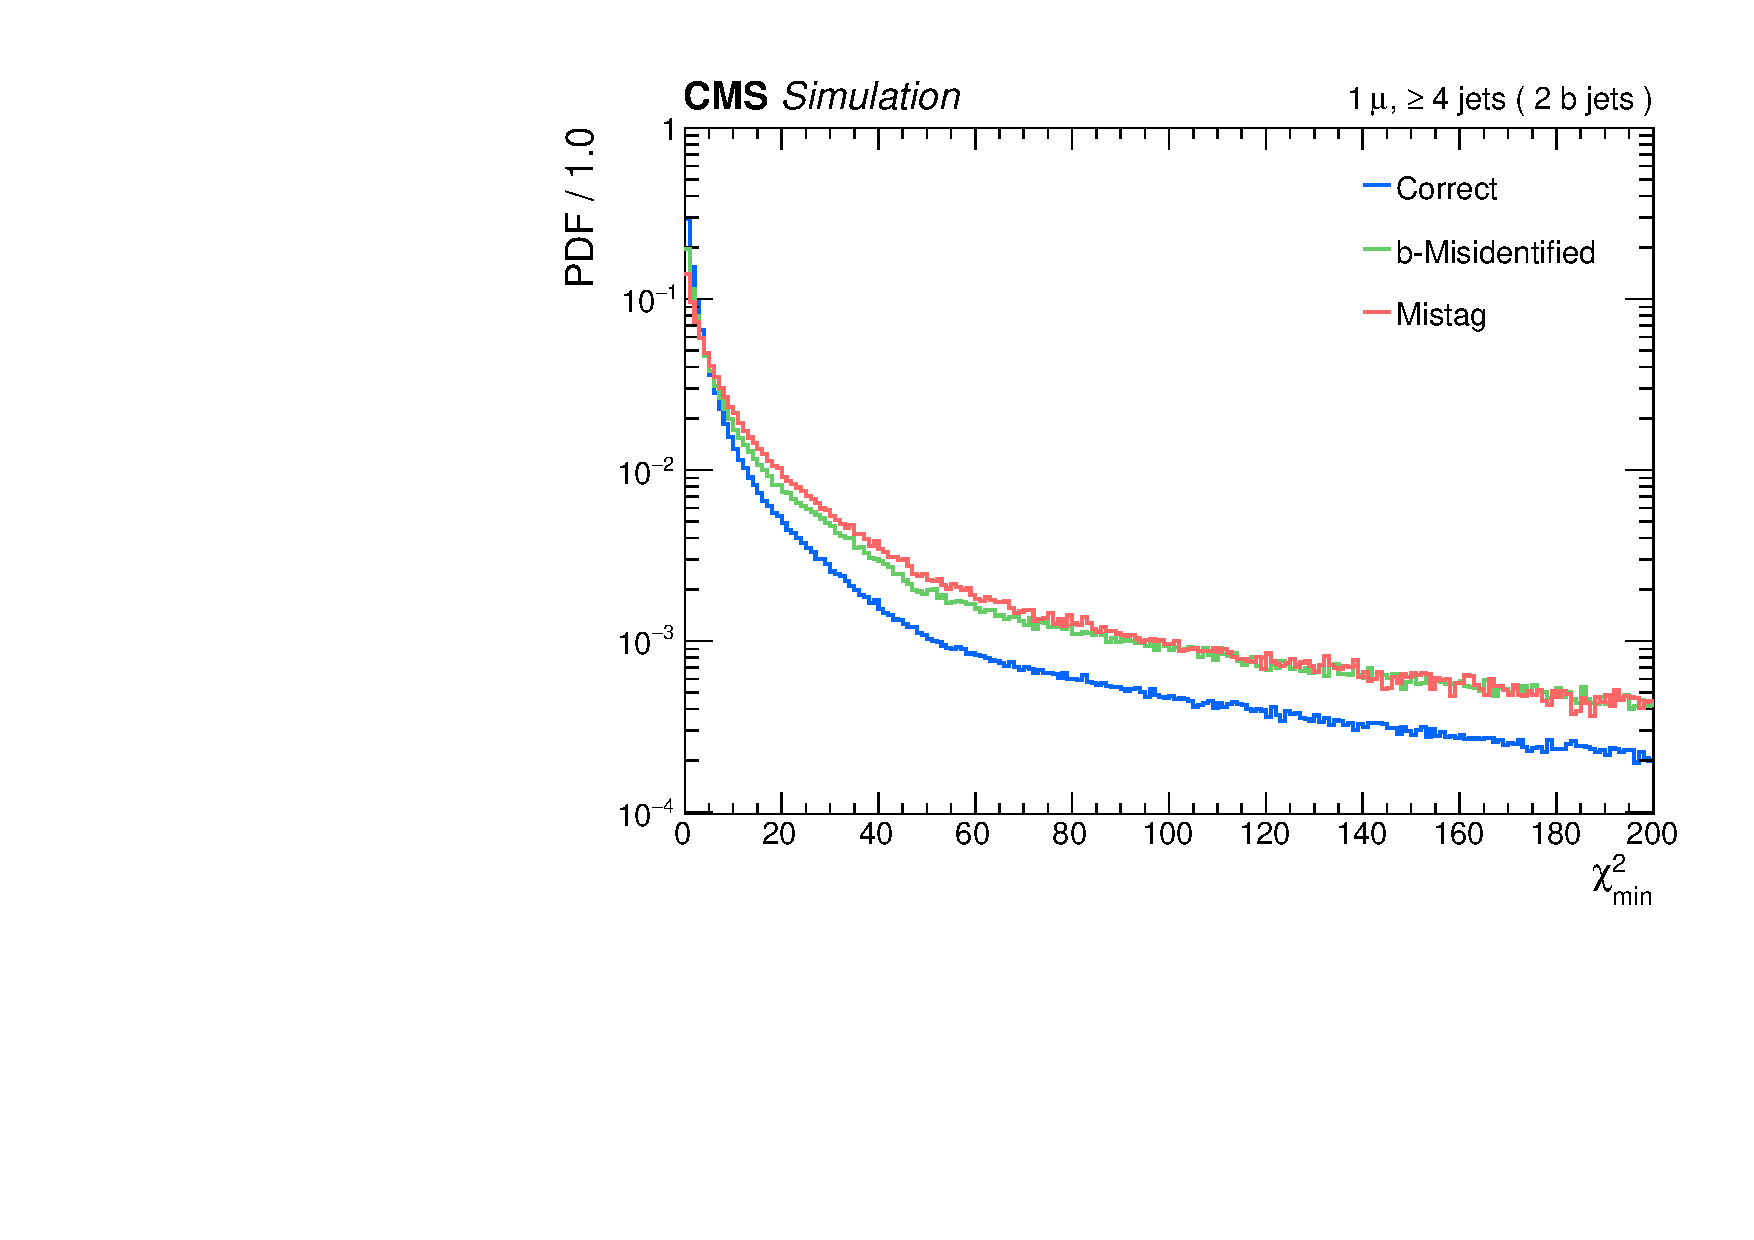
\includegraphics[width=0.45\textwidth]{figure/bbSep_18_mu_Rate_PDF_bbSep.pdf}
    \caption[The fraction of different event types in the minimum \chisq distribution.]
    {
        The fraction of different event types in the minimum \chisq distribution in electron channel (left) and muon channel (right) for 2016 (top), 2017 (middle), and 2018 (bottom) samples.
    }
    \label{fig:bbsep_rate}
\end{figure}

\begin{figure}[p]
    \centering
    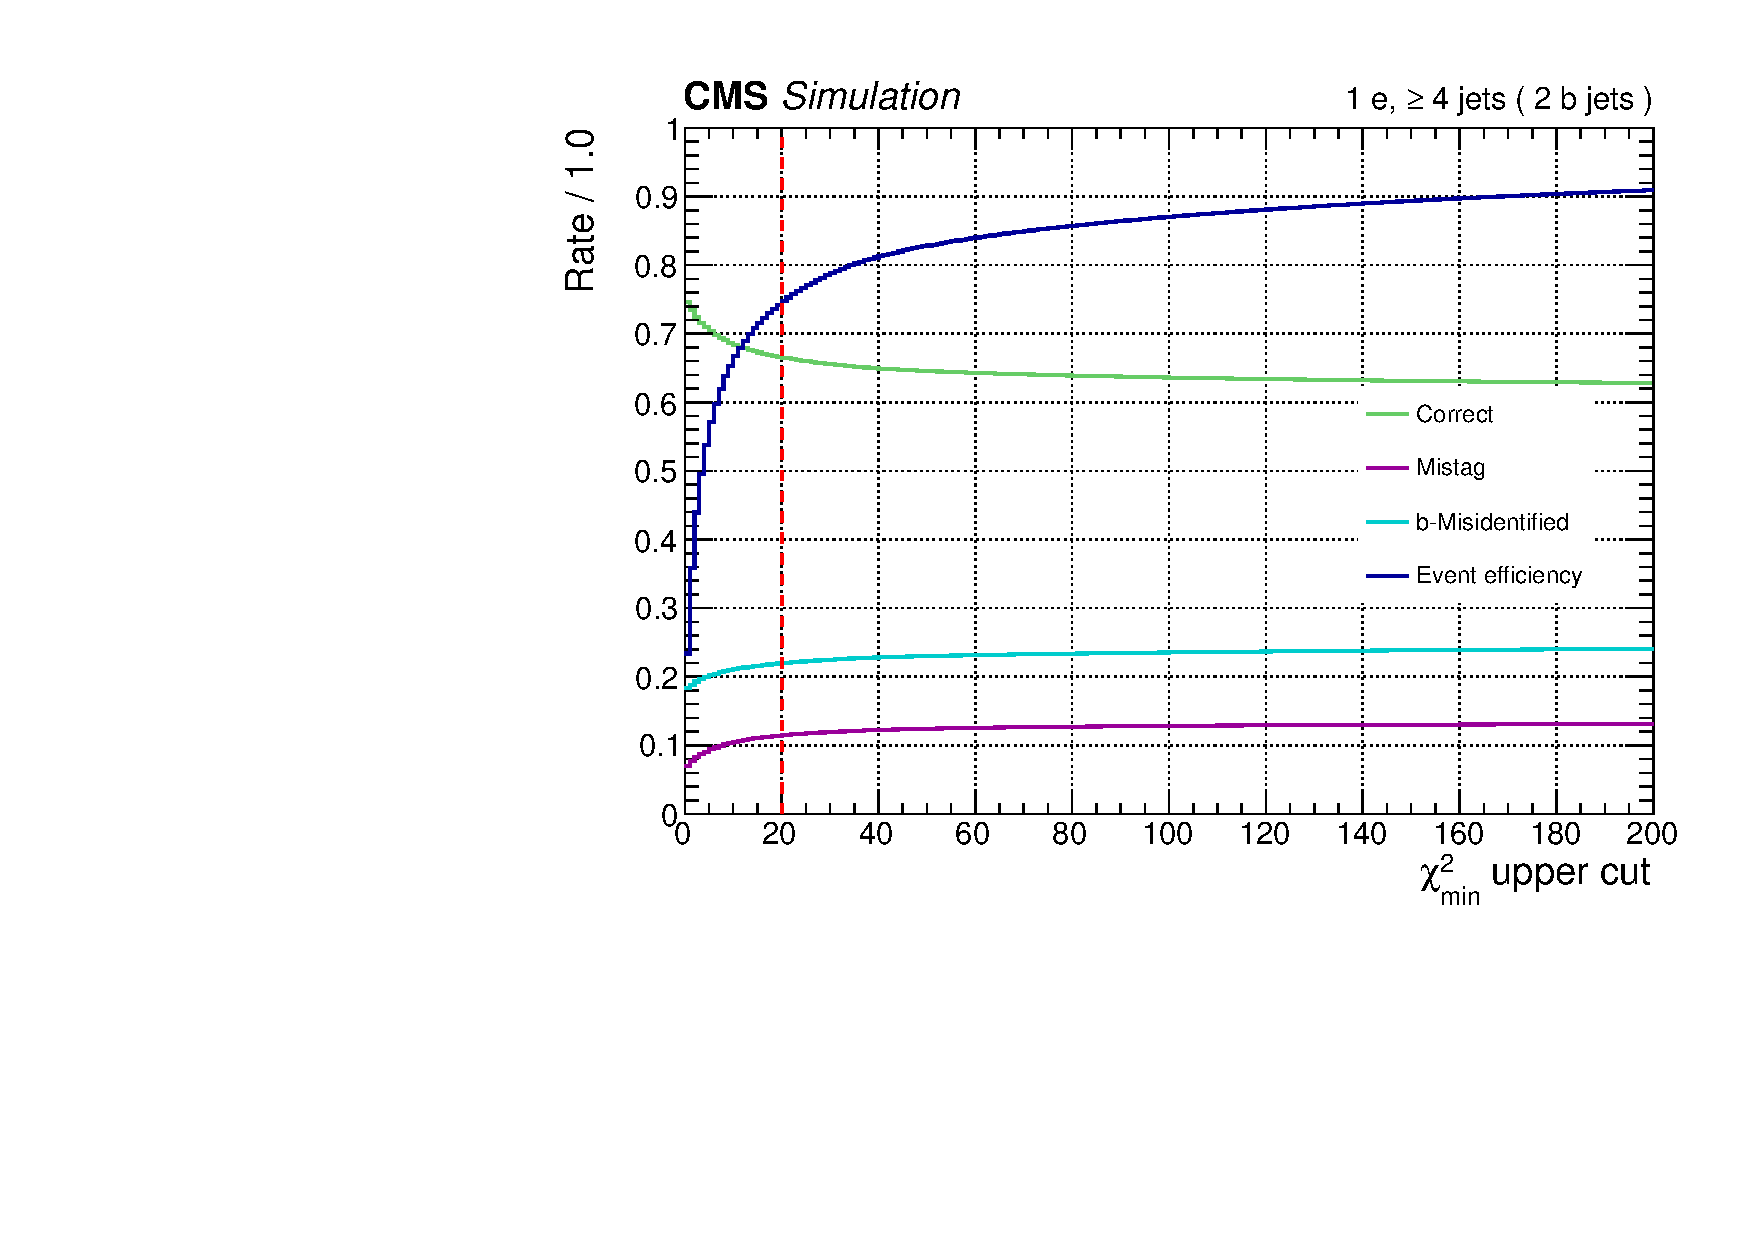
\includegraphics[width=0.45\textwidth]{figure/bbSep_16_el_Chi2_uppercut_bbSep.pdf}
    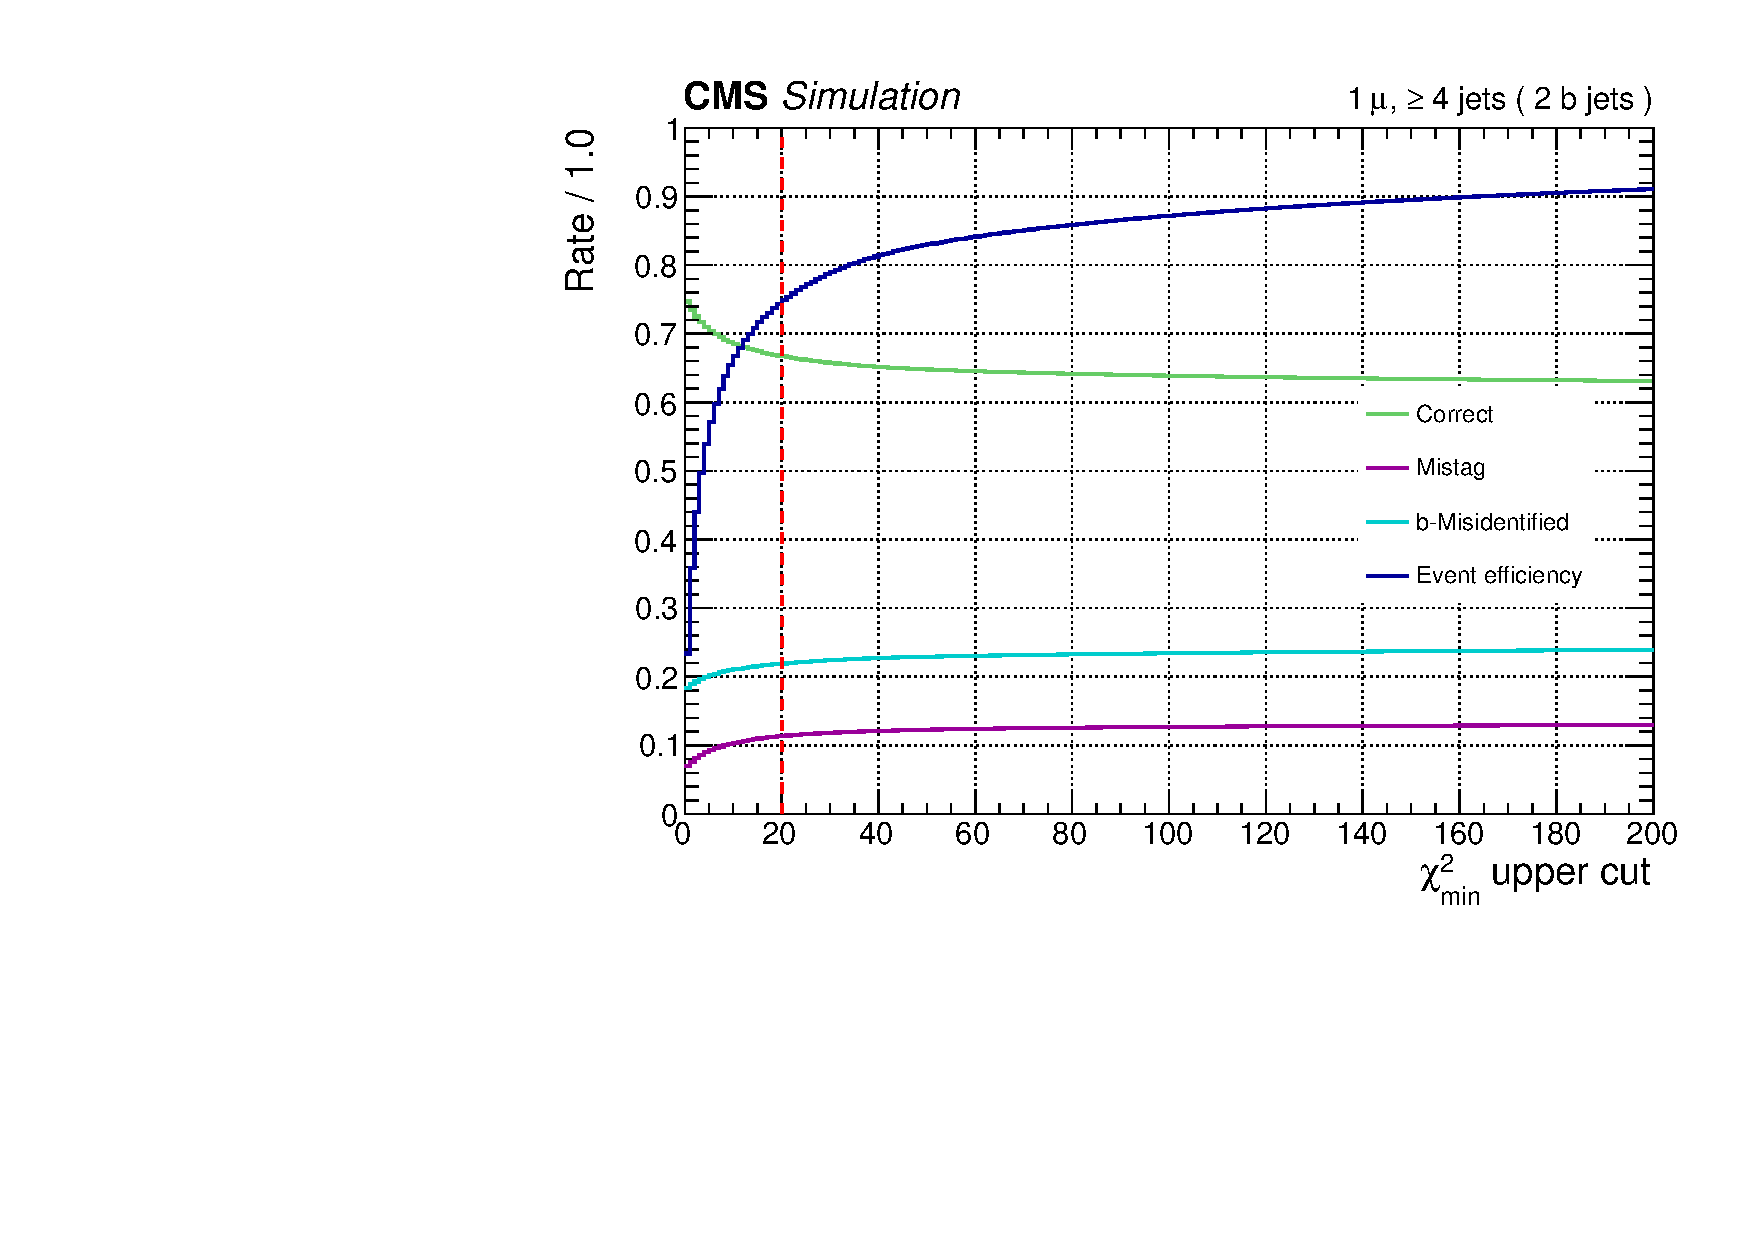
\includegraphics[width=0.45\textwidth]{figure/bbSep_16_mu_Chi2_uppercut_bbSep.pdf}
    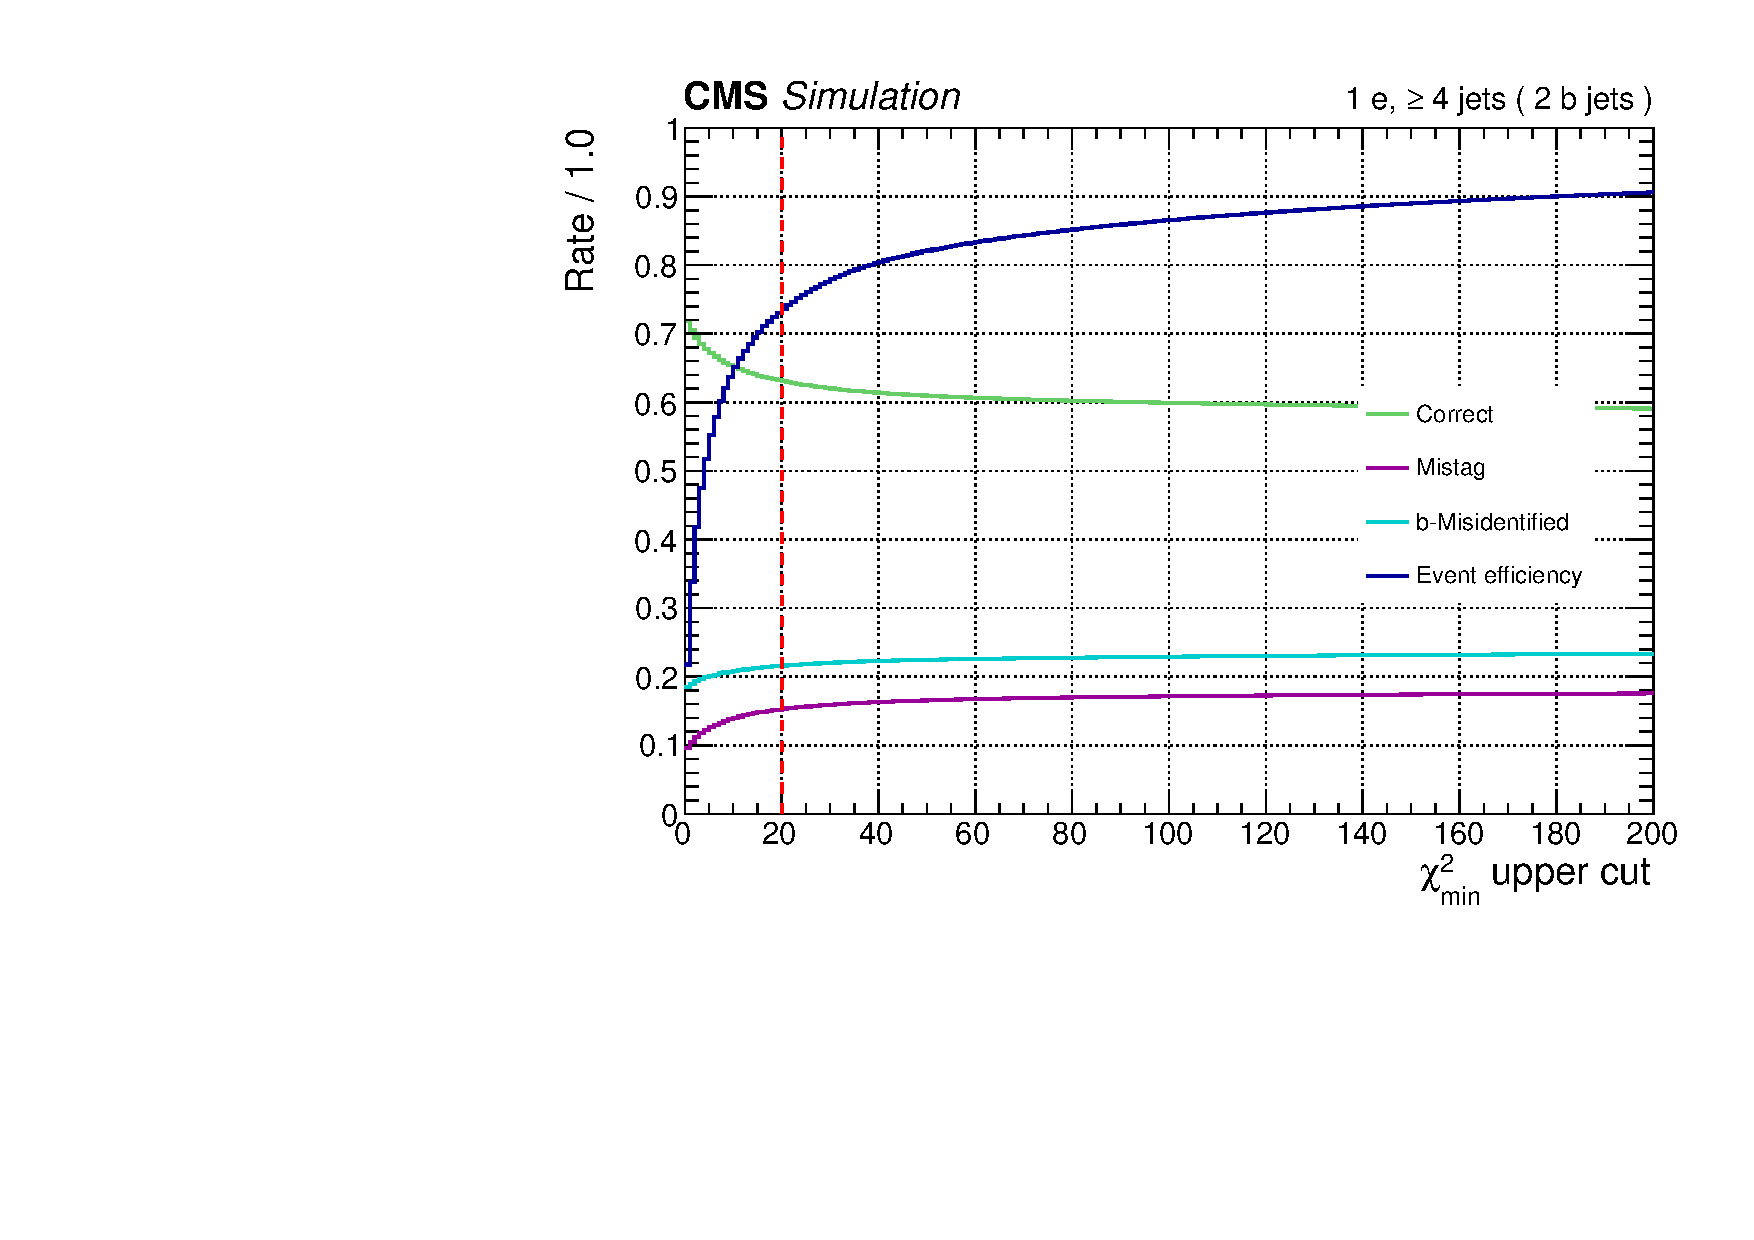
\includegraphics[width=0.45\textwidth]{figure/bbSep_17_el_Chi2_uppercut_bbSep.pdf}
    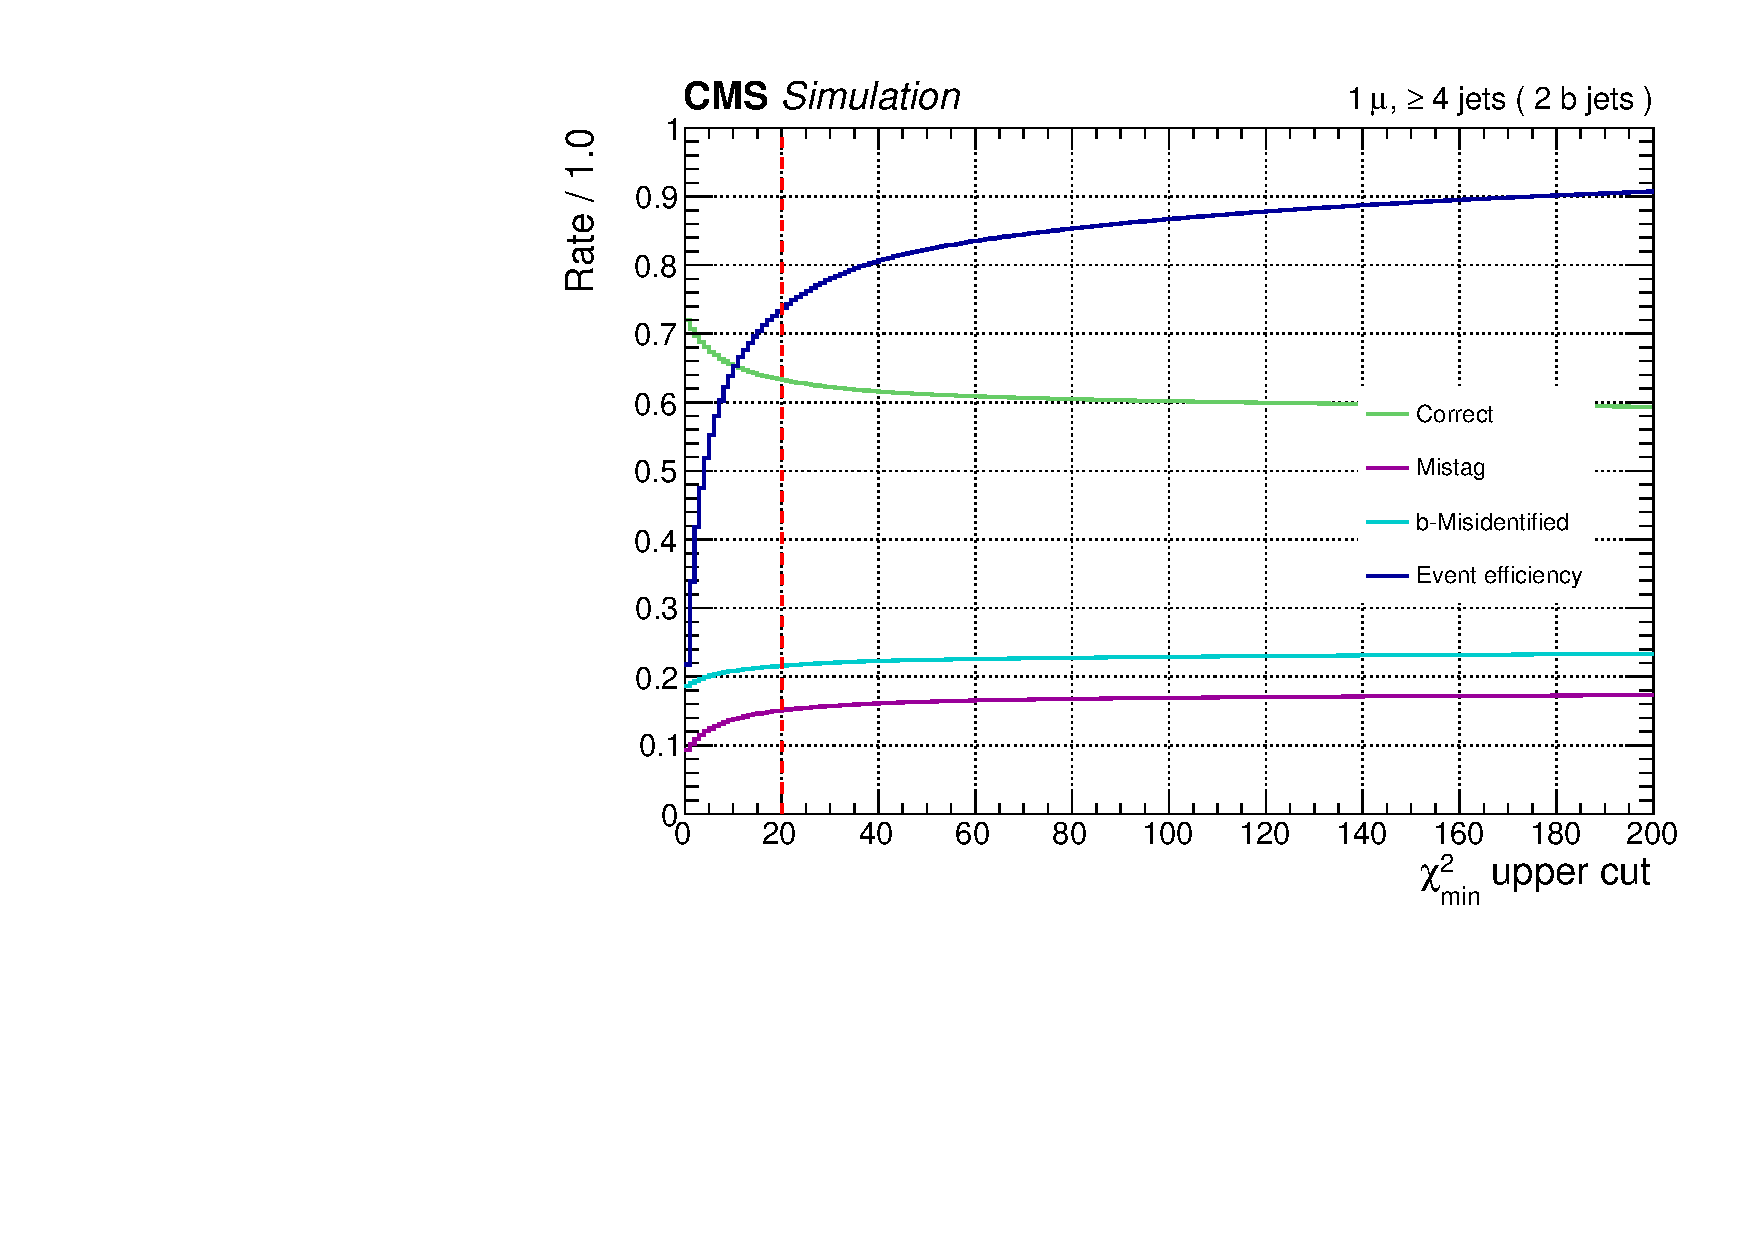
\includegraphics[width=0.45\textwidth]{figure/bbSep_17_mu_Chi2_uppercut_bbSep.pdf}
    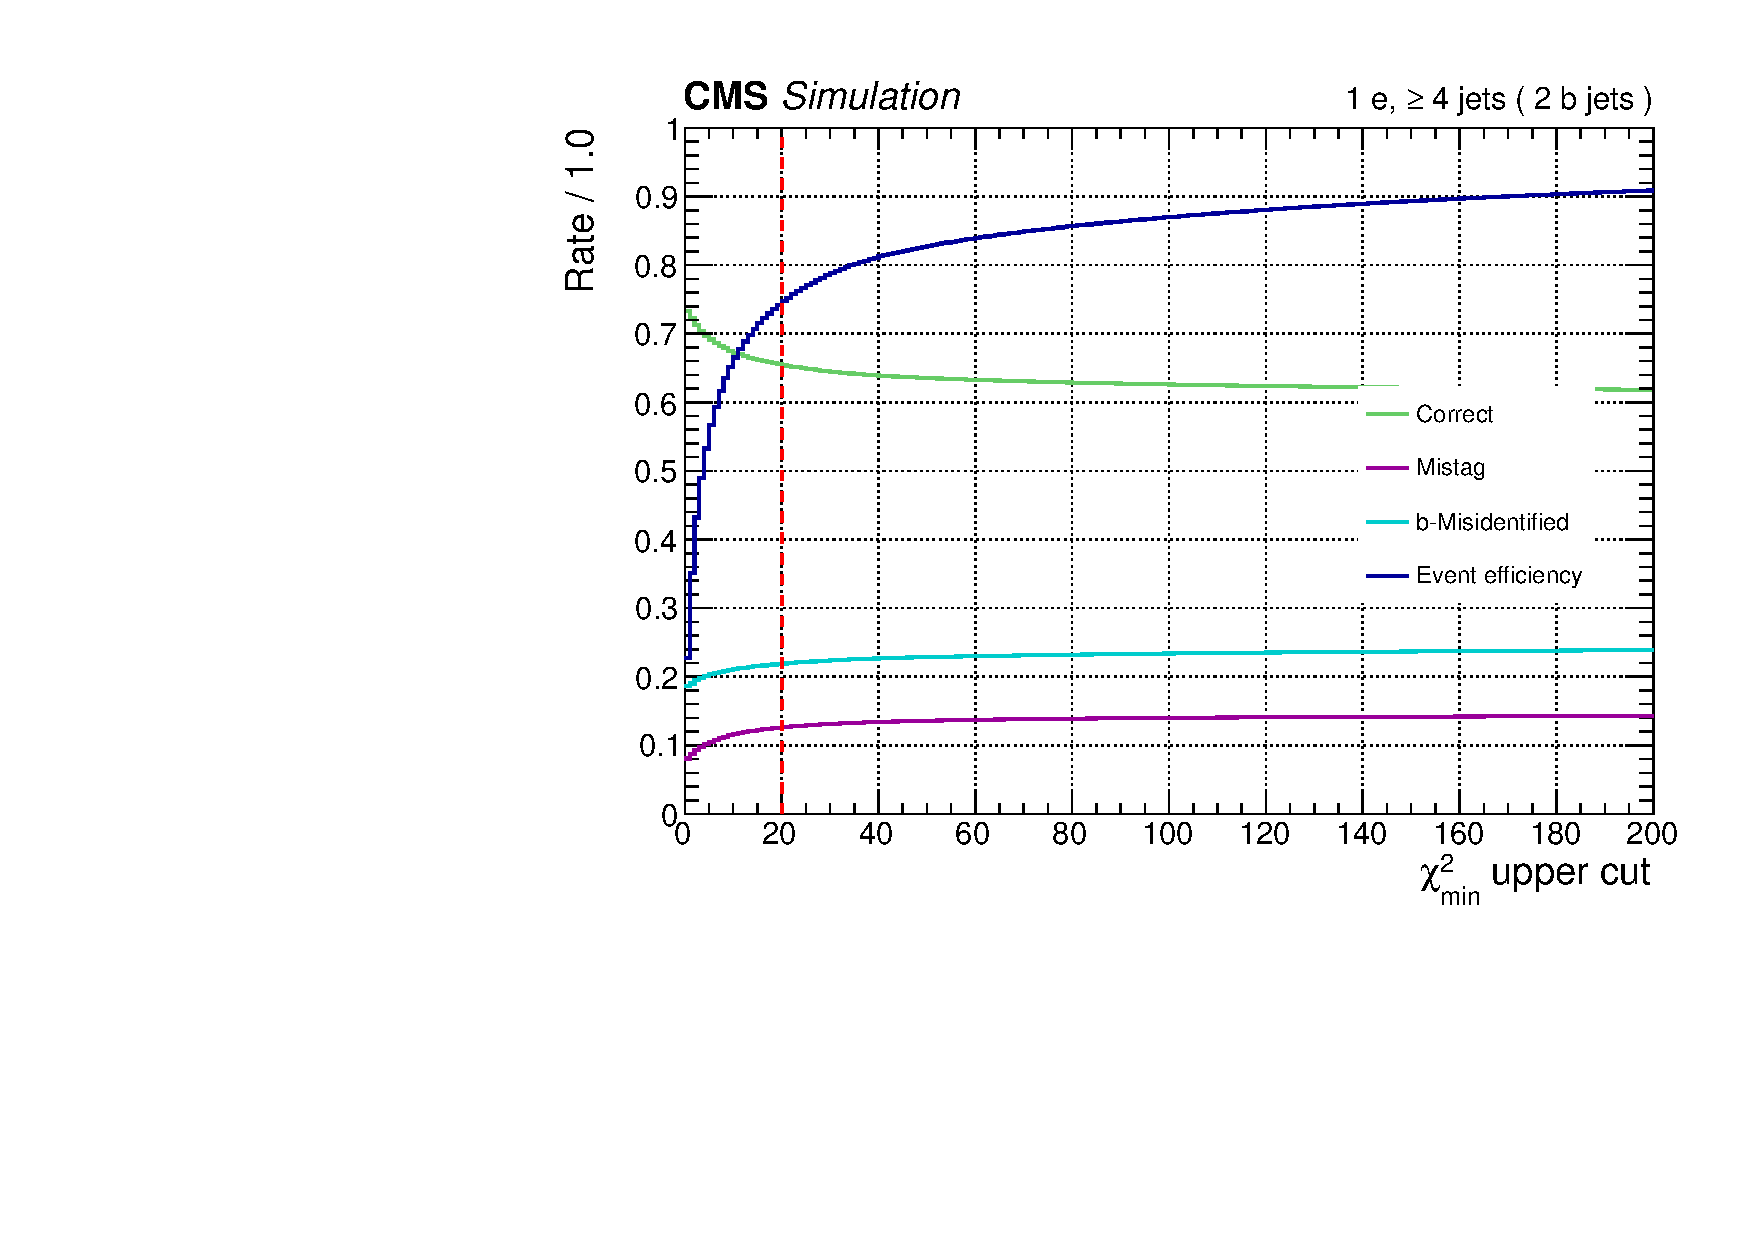
\includegraphics[width=0.45\textwidth]{figure/bbSep_18_el_Chi2_uppercut_bbSep.pdf}
    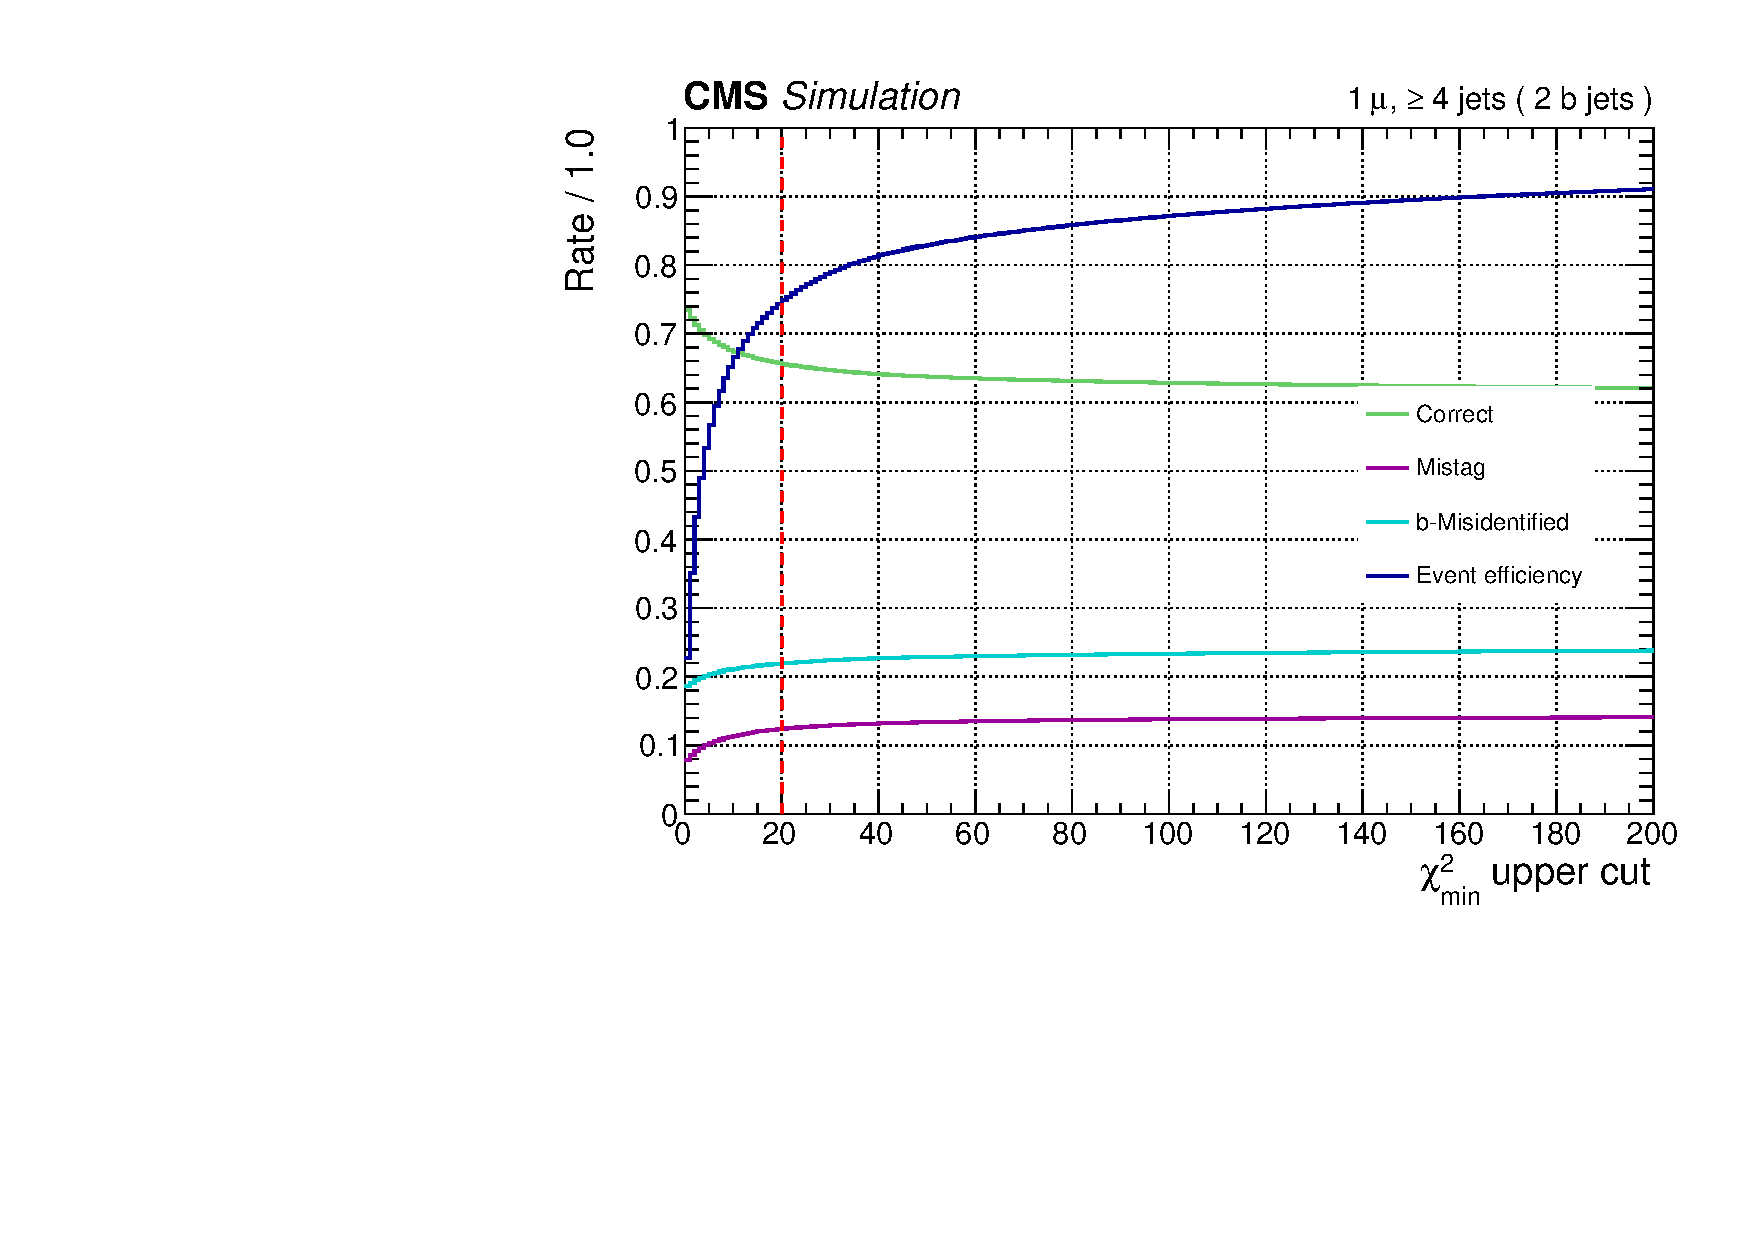
\includegraphics[width=0.45\textwidth]{figure/bbSep_18_mu_Chi2_uppercut_bbSep.pdf}
    \caption[The fraction of different event types in the distribution of the upper bound on minimum \chisq.]
    {
        The fraction of different event types in the distribution of upper bound on \chisq in electron channel (left) and muon channel (right) for 2016 (top), 2017 (middle), and 2018 (bottom) samples.
        The red dotted line shows the used uppeer bound in this analysis.
    }
    \label{fig:bbsep_uppercut}
\end{figure}

\begin{figure}[p]
    \centering
    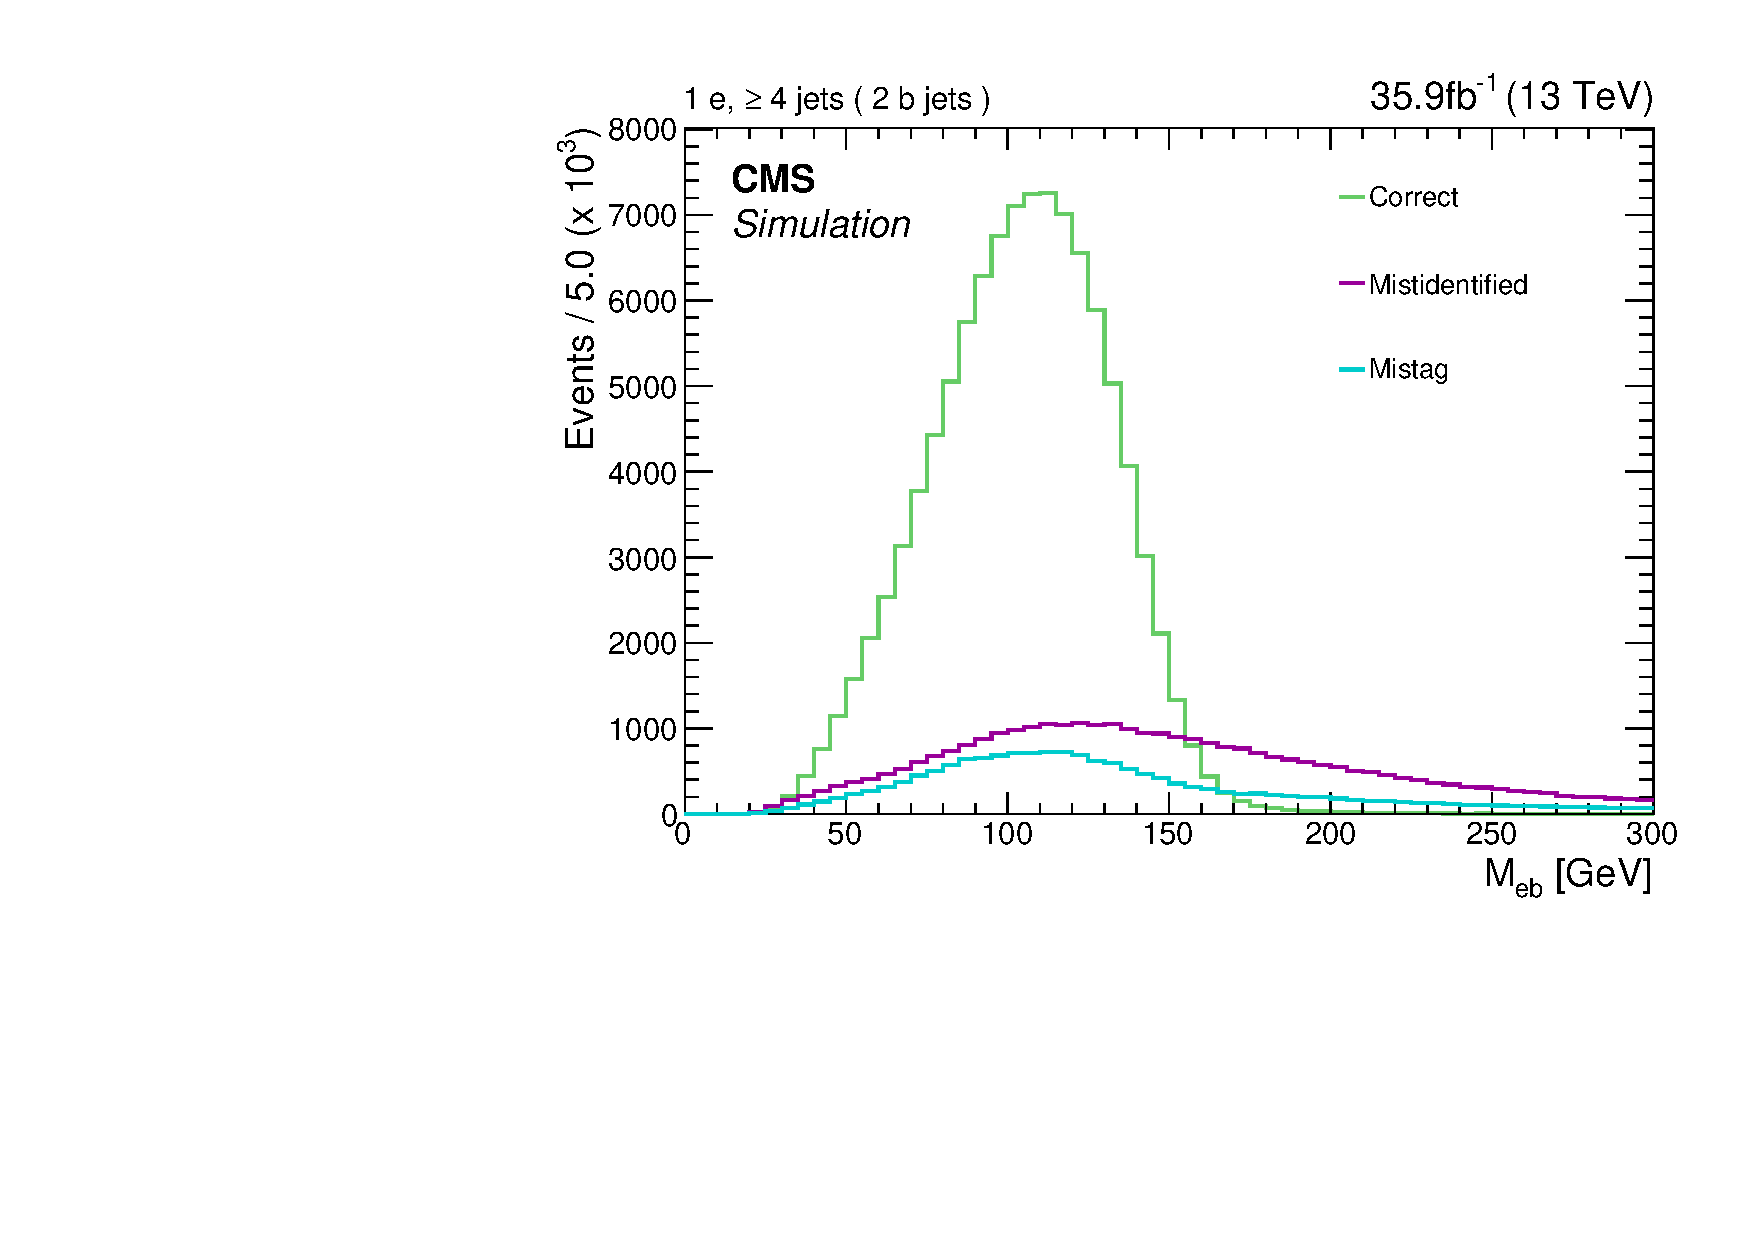
\includegraphics[width=0.45\textwidth]{figure/bbSep_16_el_Optimisation_chi2_20_bbSep.pdf}
    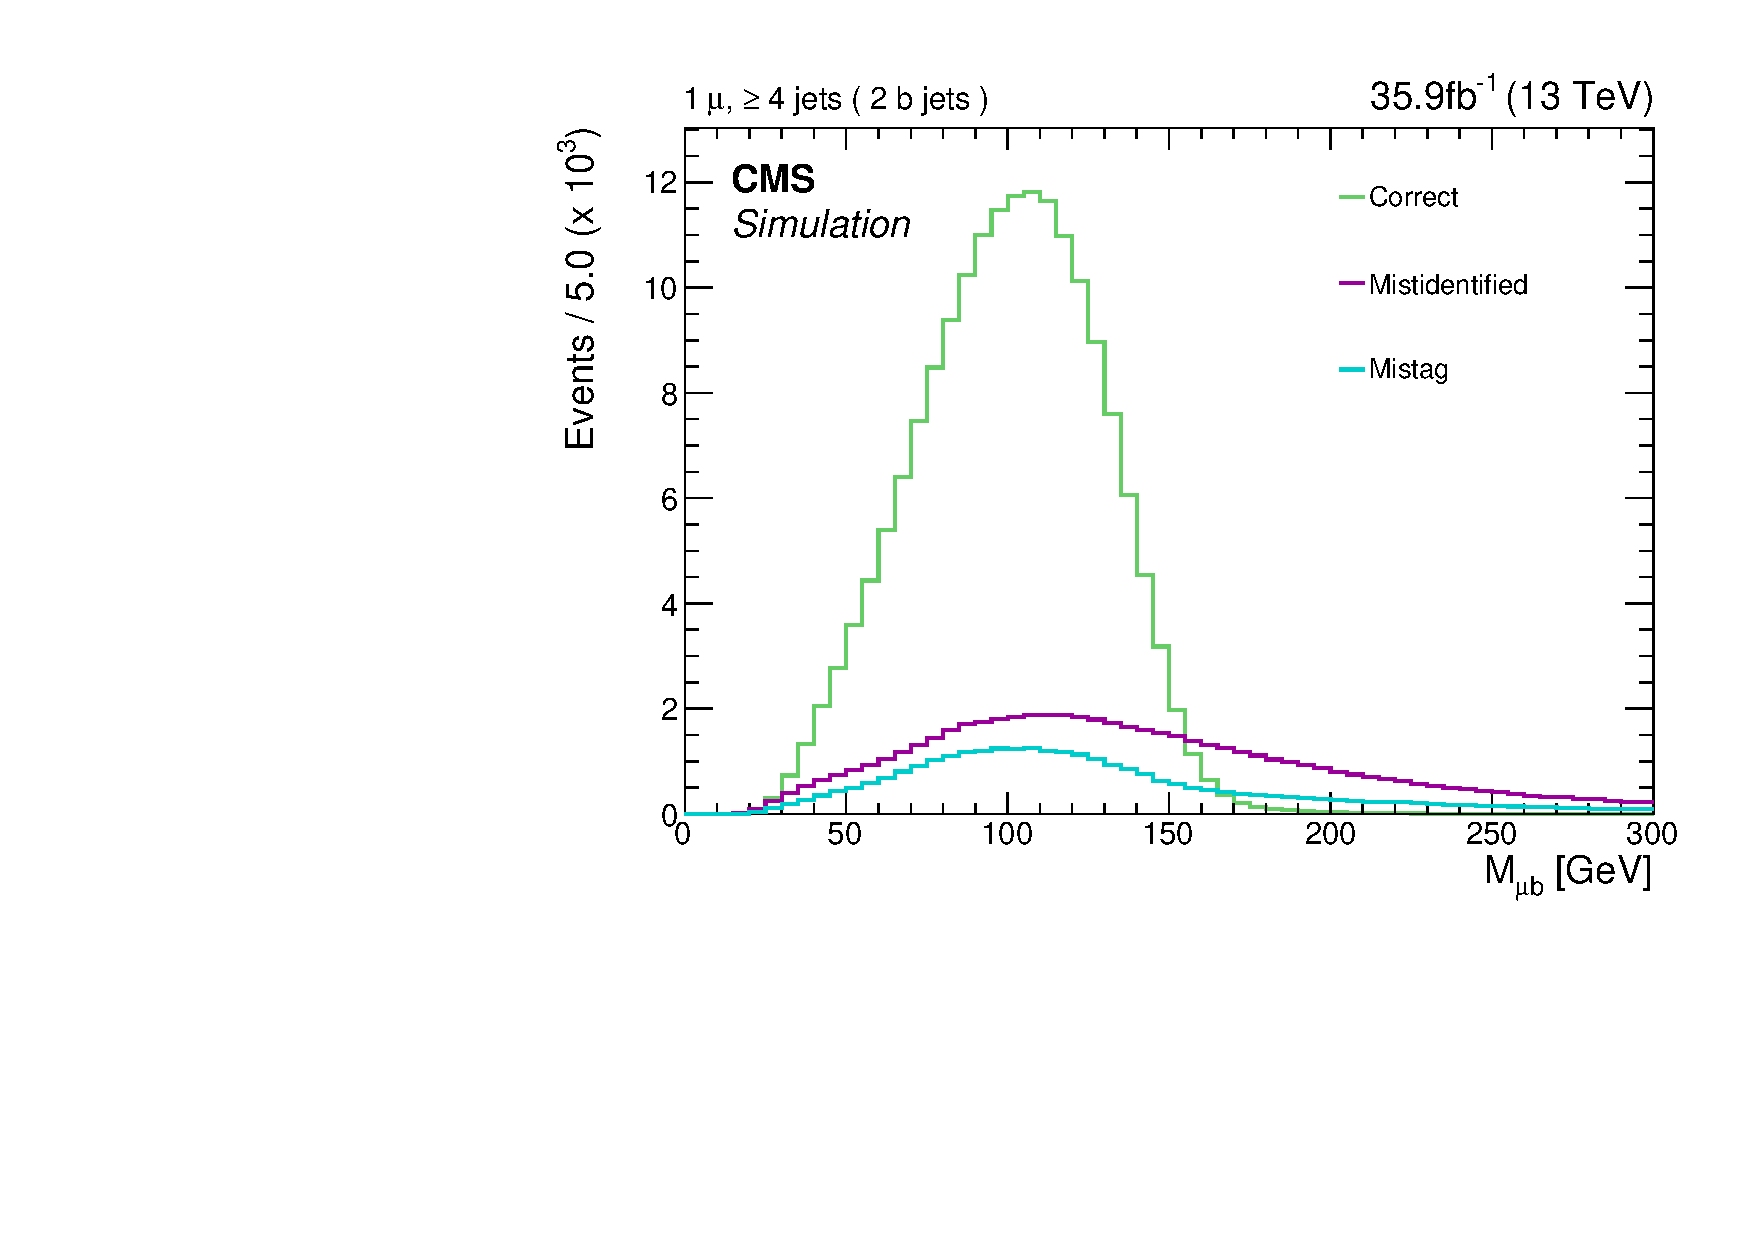
\includegraphics[width=0.45\textwidth]{figure/bbSep_16_mu_Optimisation_chi2_20_bbSep.pdf}
    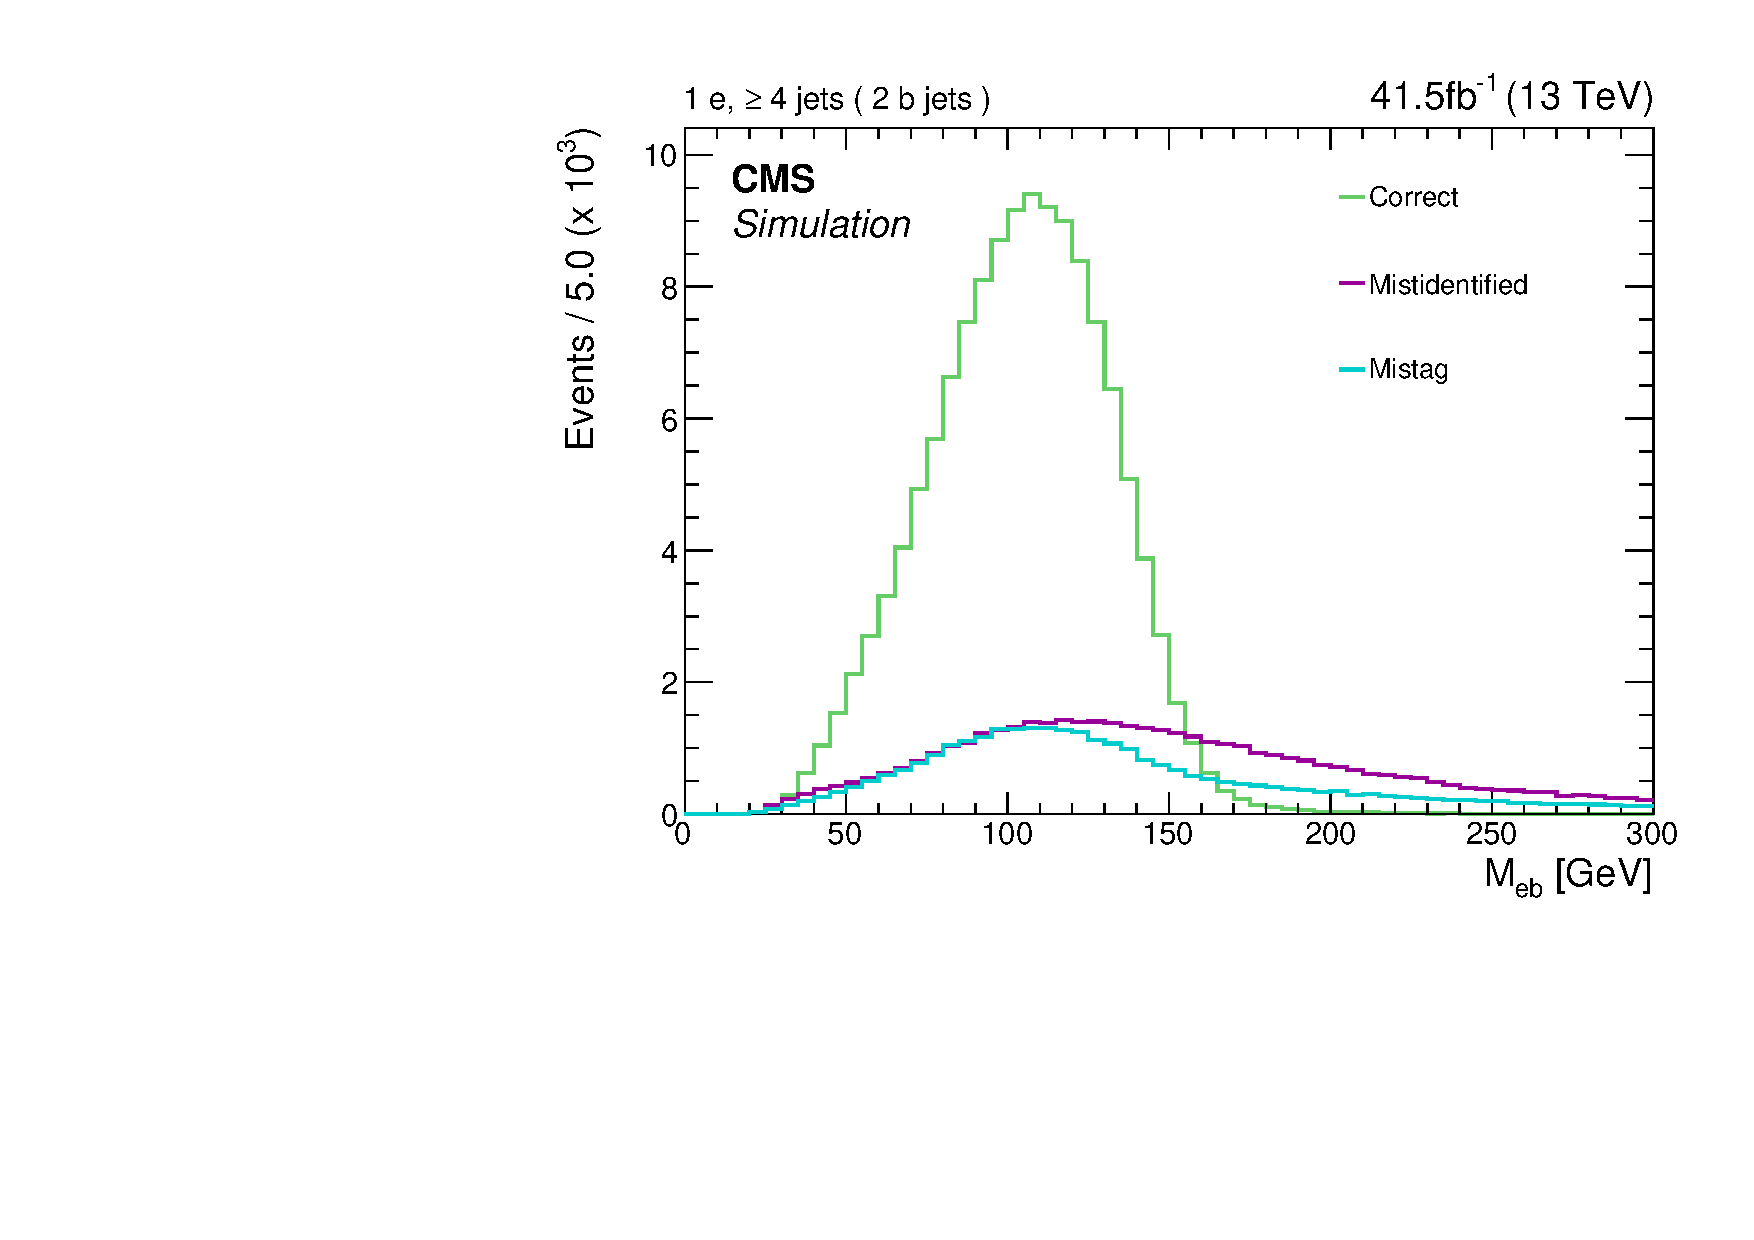
\includegraphics[width=0.45\textwidth]{figure/bbSep_17_el_Optimisation_chi2_20_bbSep.pdf}
    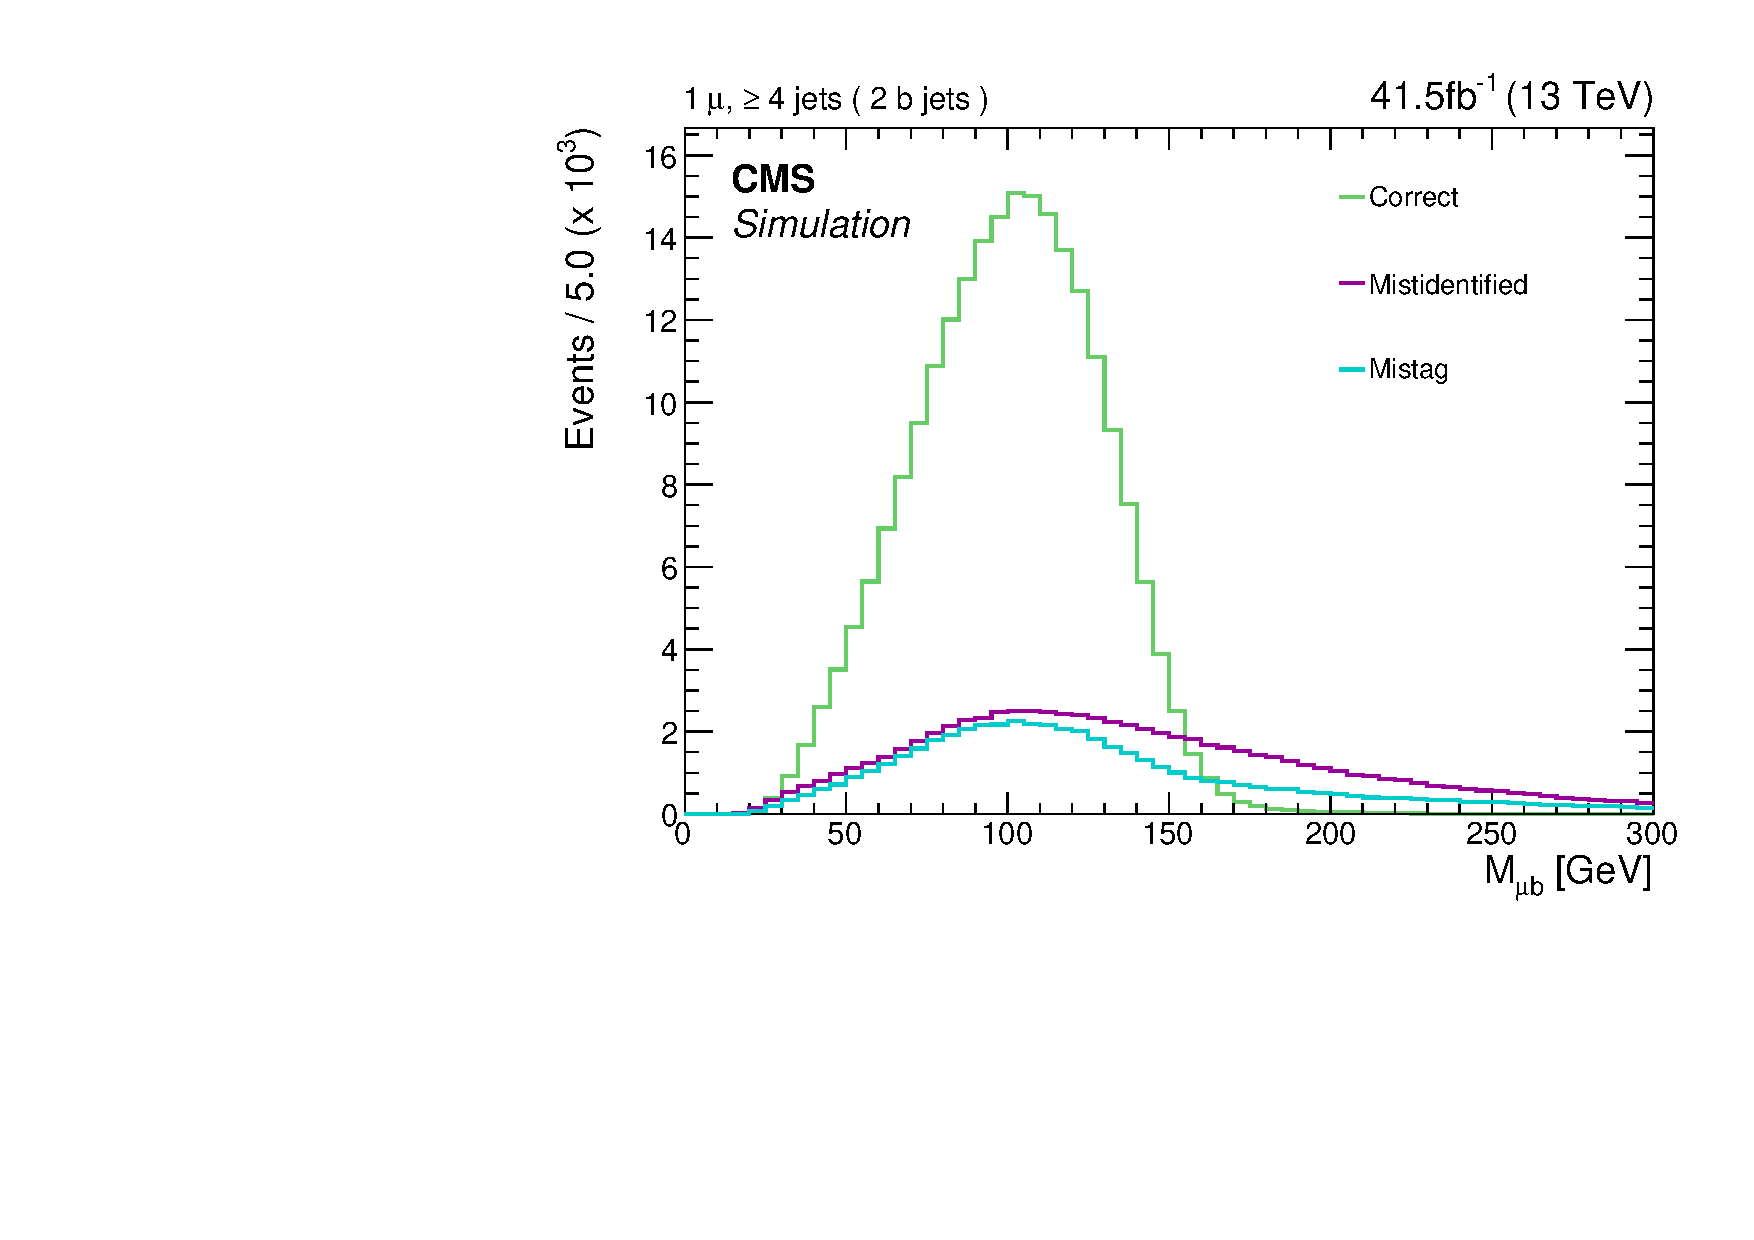
\includegraphics[width=0.45\textwidth]{figure/bbSep_17_mu_Optimisation_chi2_20_bbSep.pdf}
    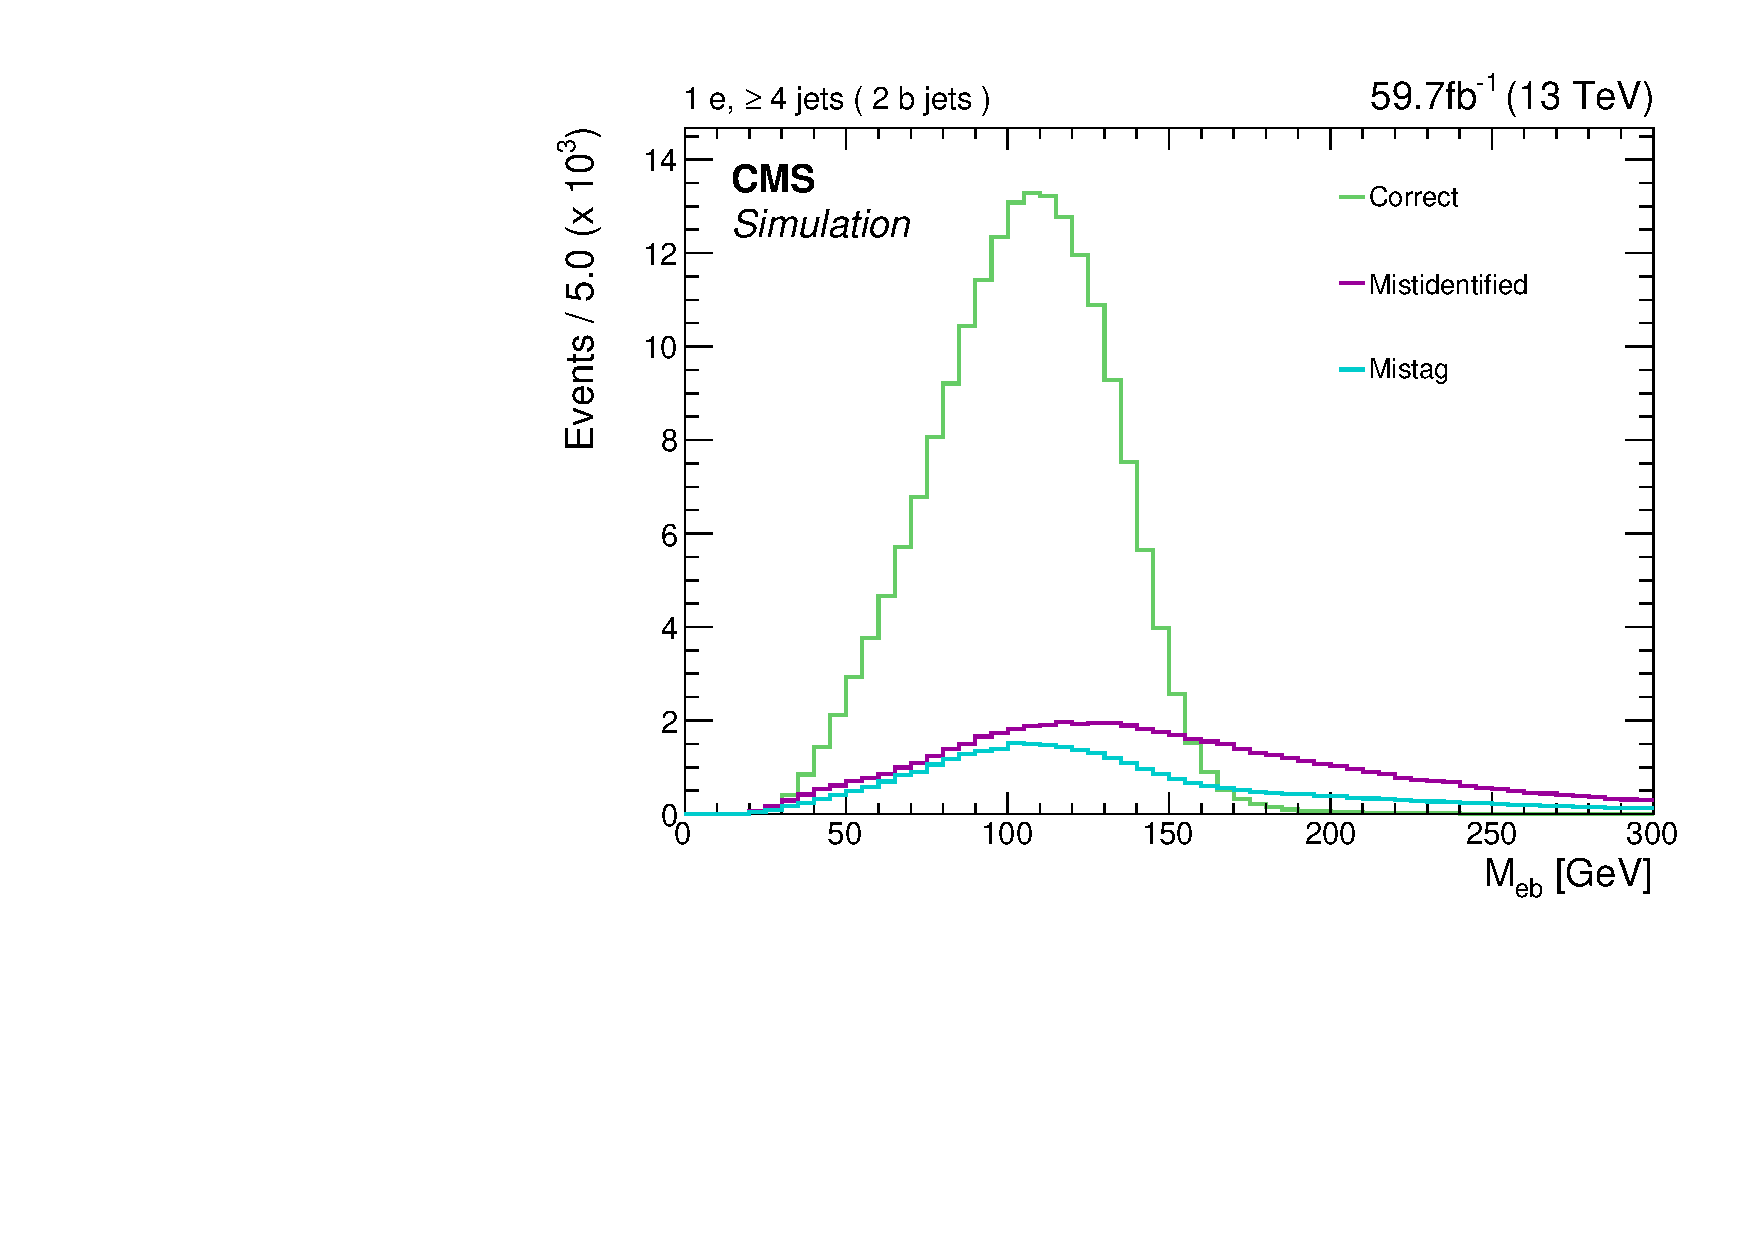
\includegraphics[width=0.45\textwidth]{figure/bbSep_18_el_Optimisation_chi2_20_bbSep.pdf}
    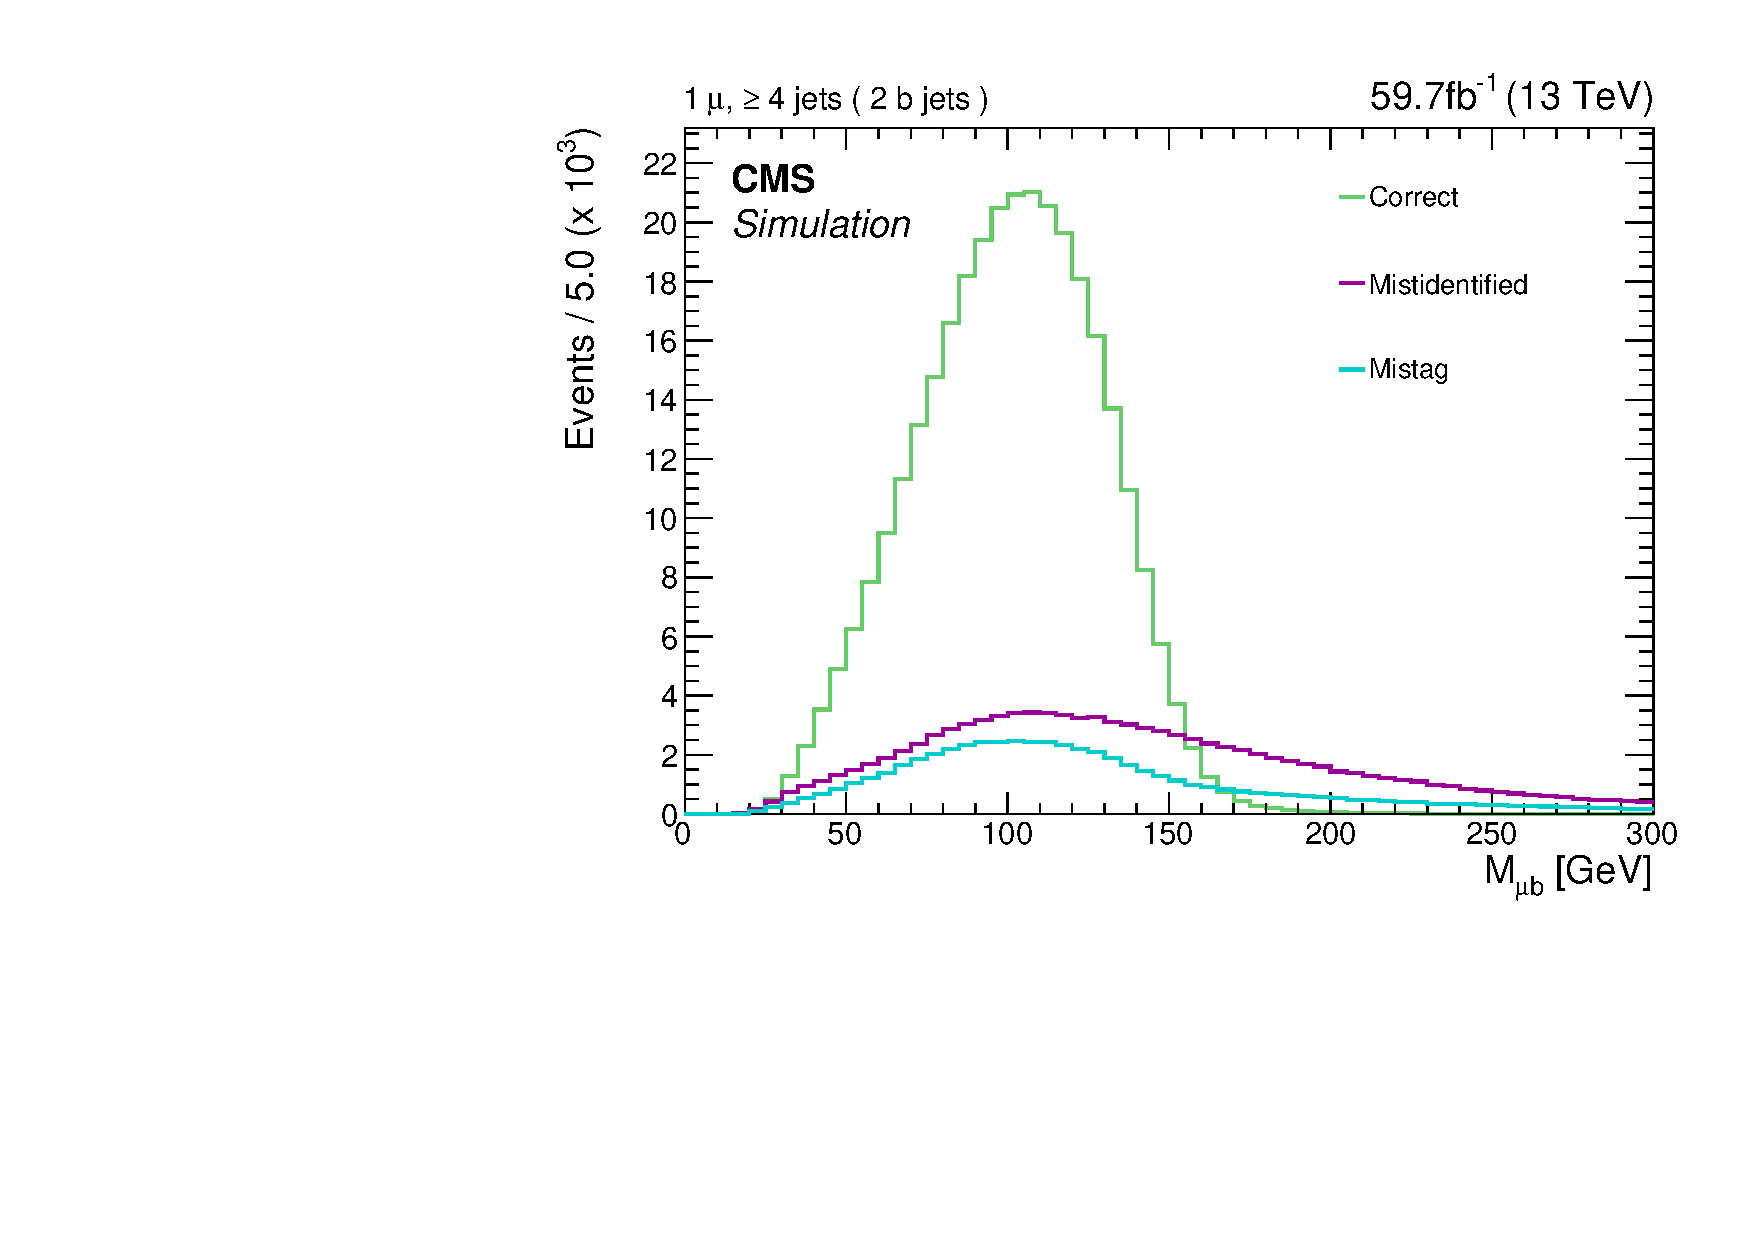
\includegraphics[width=0.45\textwidth]{figure/bbSep_18_mu_Optimisation_chi2_20_bbSep.pdf}
    \caption[The \Mlb distribution of different event types.]
    {
        The \Mlb distribution of different event type in electron channel (left) and muon channel (right) for 2016 (top), 2017 (middle), and 2018 (bottom) samples.
    }
    \label{fig:opt_lept}
\end{figure}

\begin{figure}[p]
    \centering
    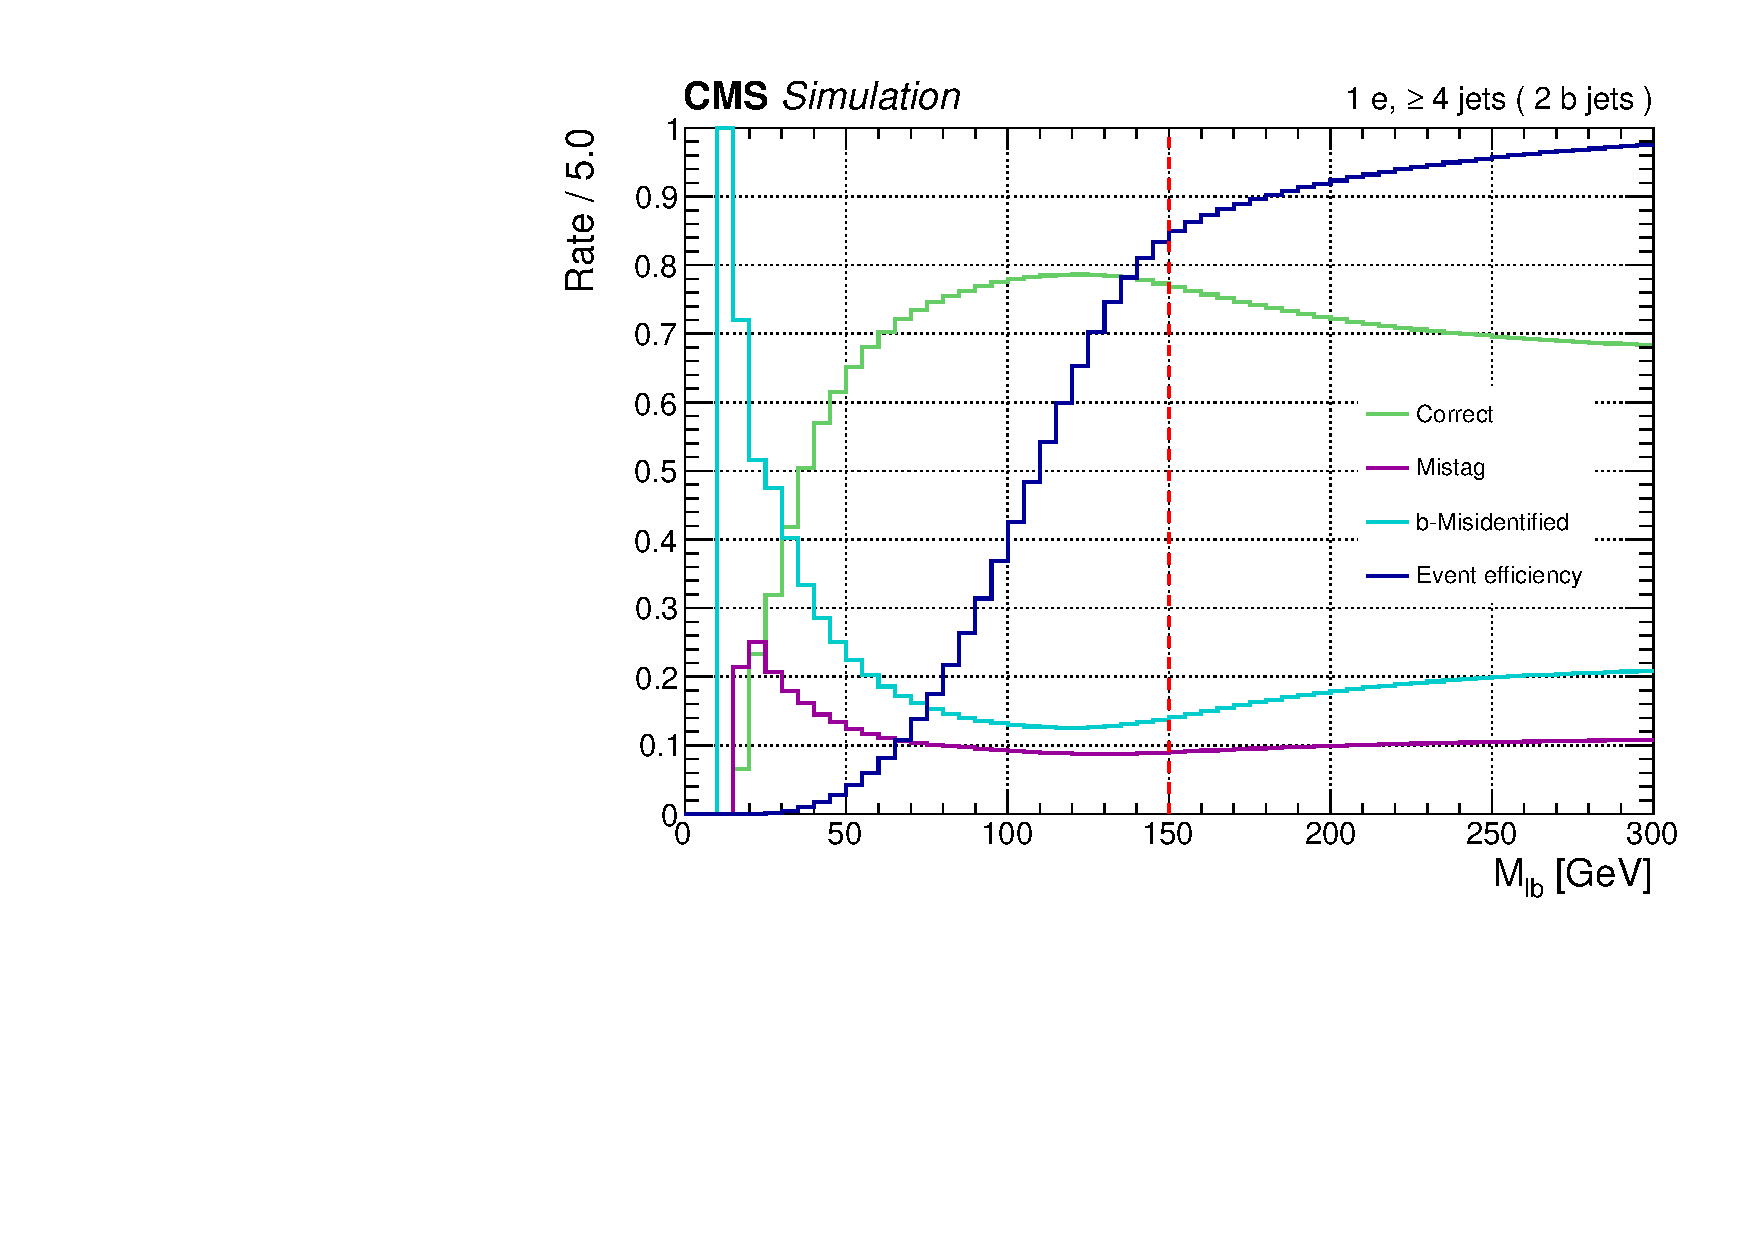
\includegraphics[width=0.45\textwidth]{figure/bbSep_16_el_OptCut_chi2_20_bbSep.pdf}
    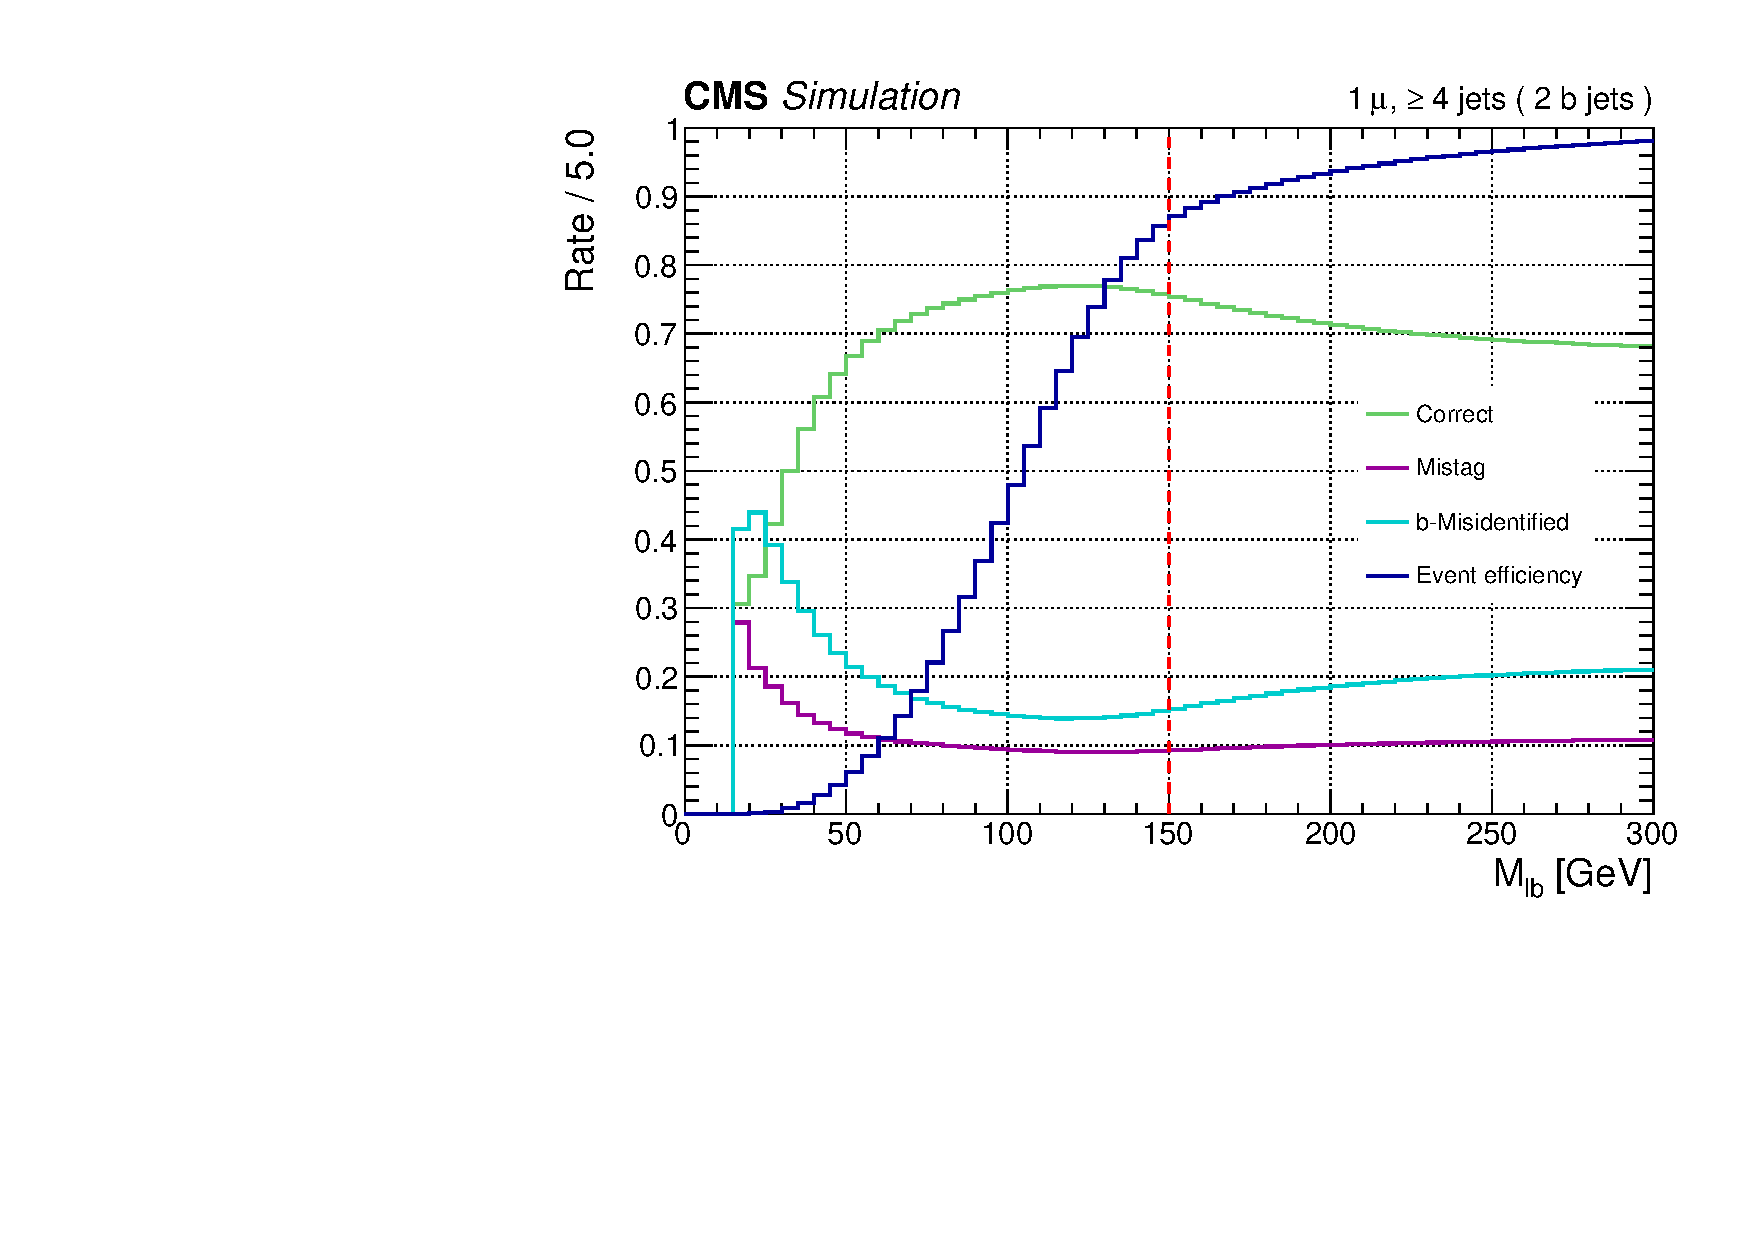
\includegraphics[width=0.45\textwidth]{figure/bbSep_16_mu_OptCut_chi2_20_bbSep.pdf}
    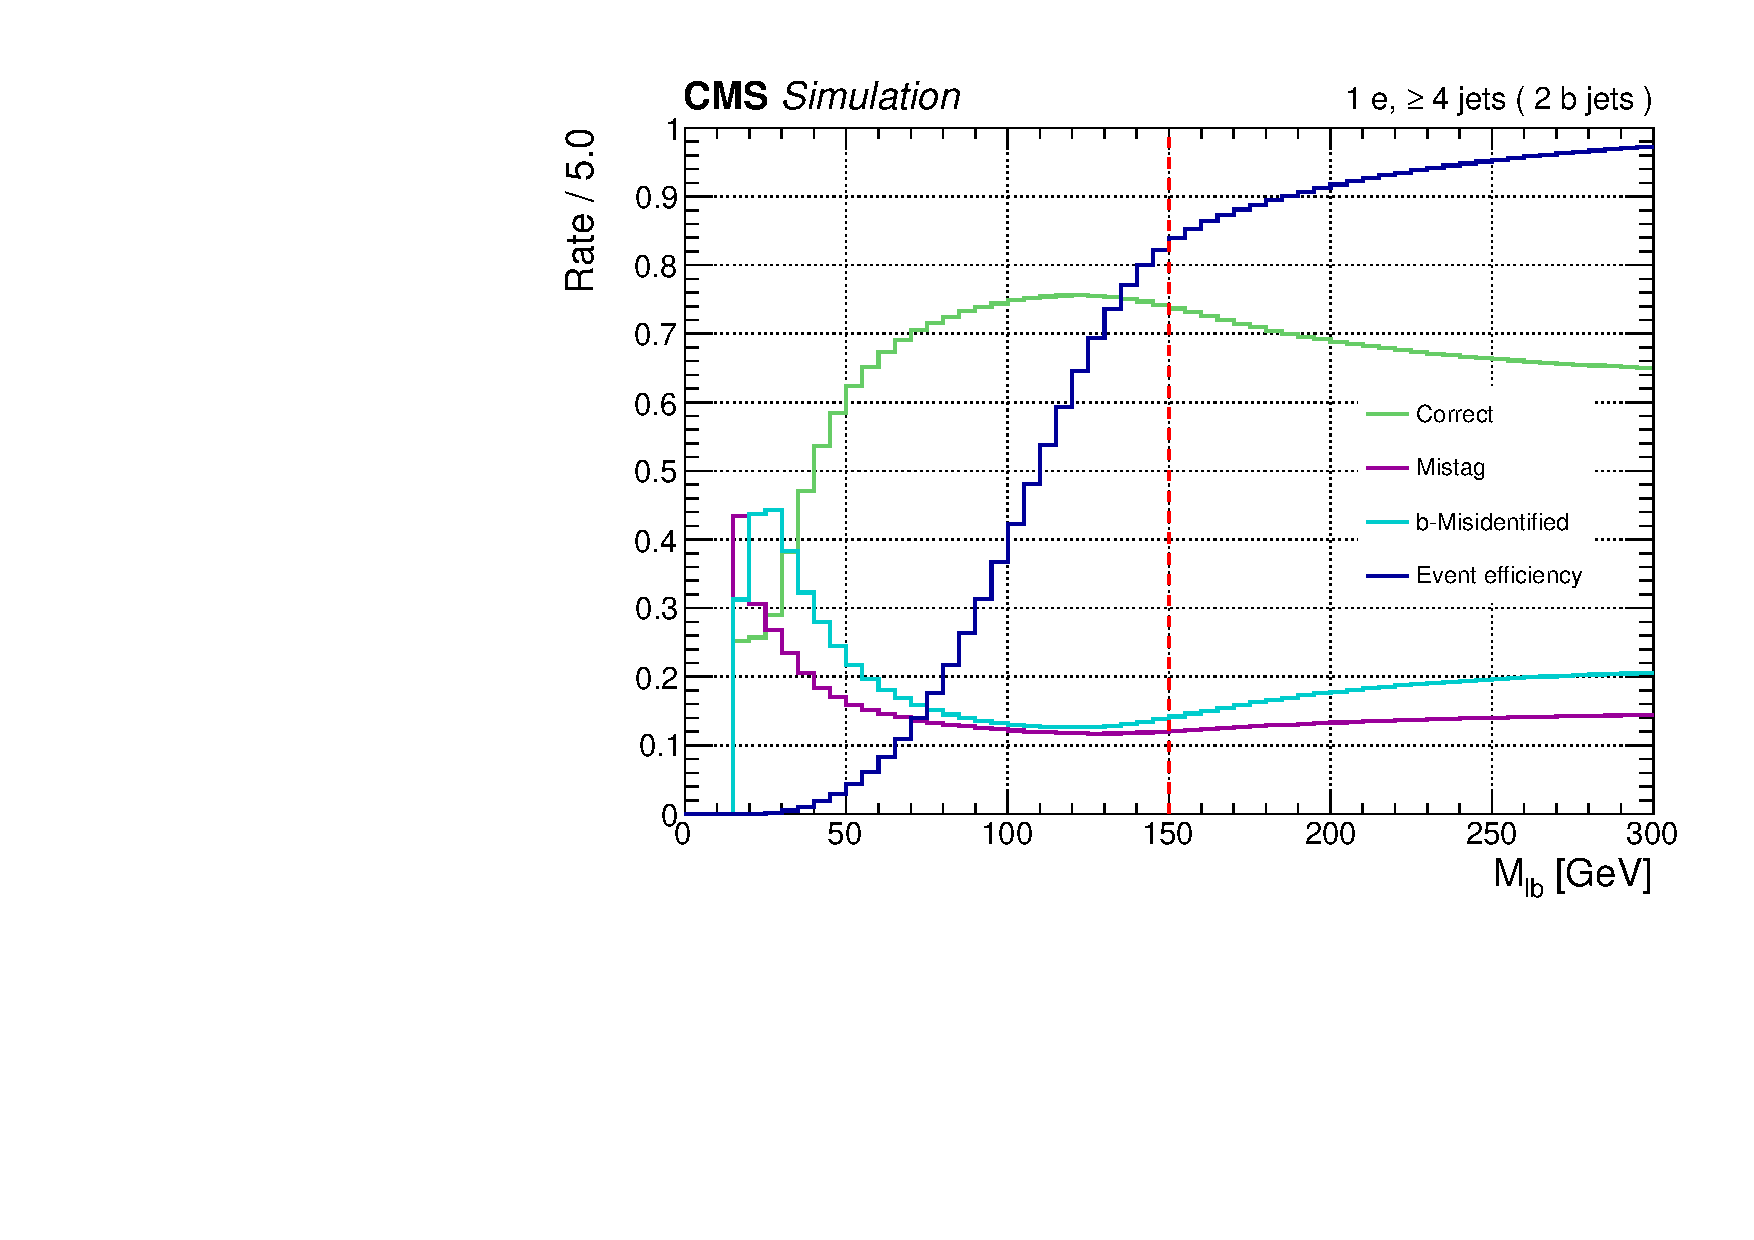
\includegraphics[width=0.45\textwidth]{figure/bbSep_17_el_OptCut_chi2_20_bbSep.pdf}
    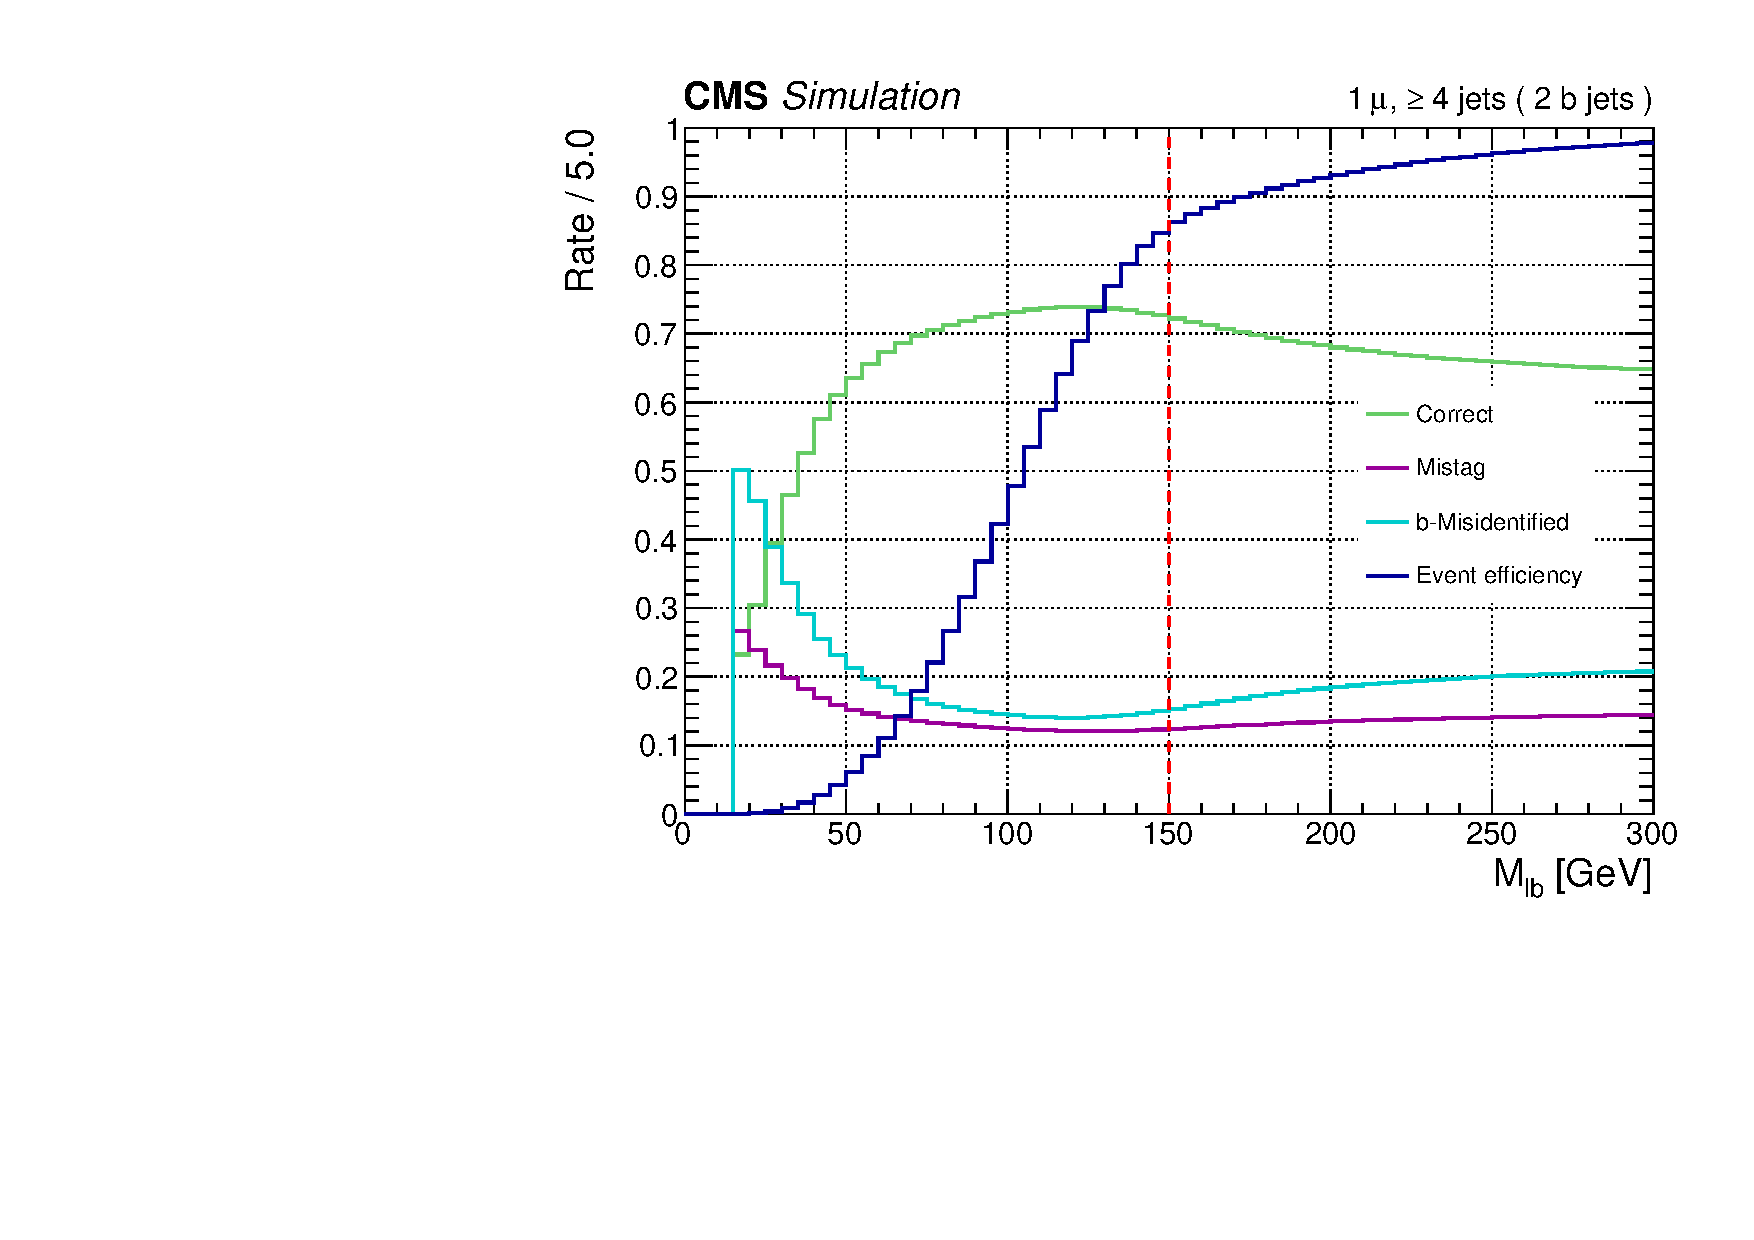
\includegraphics[width=0.45\textwidth]{figure/bbSep_17_mu_OptCut_chi2_20_bbSep.pdf}
    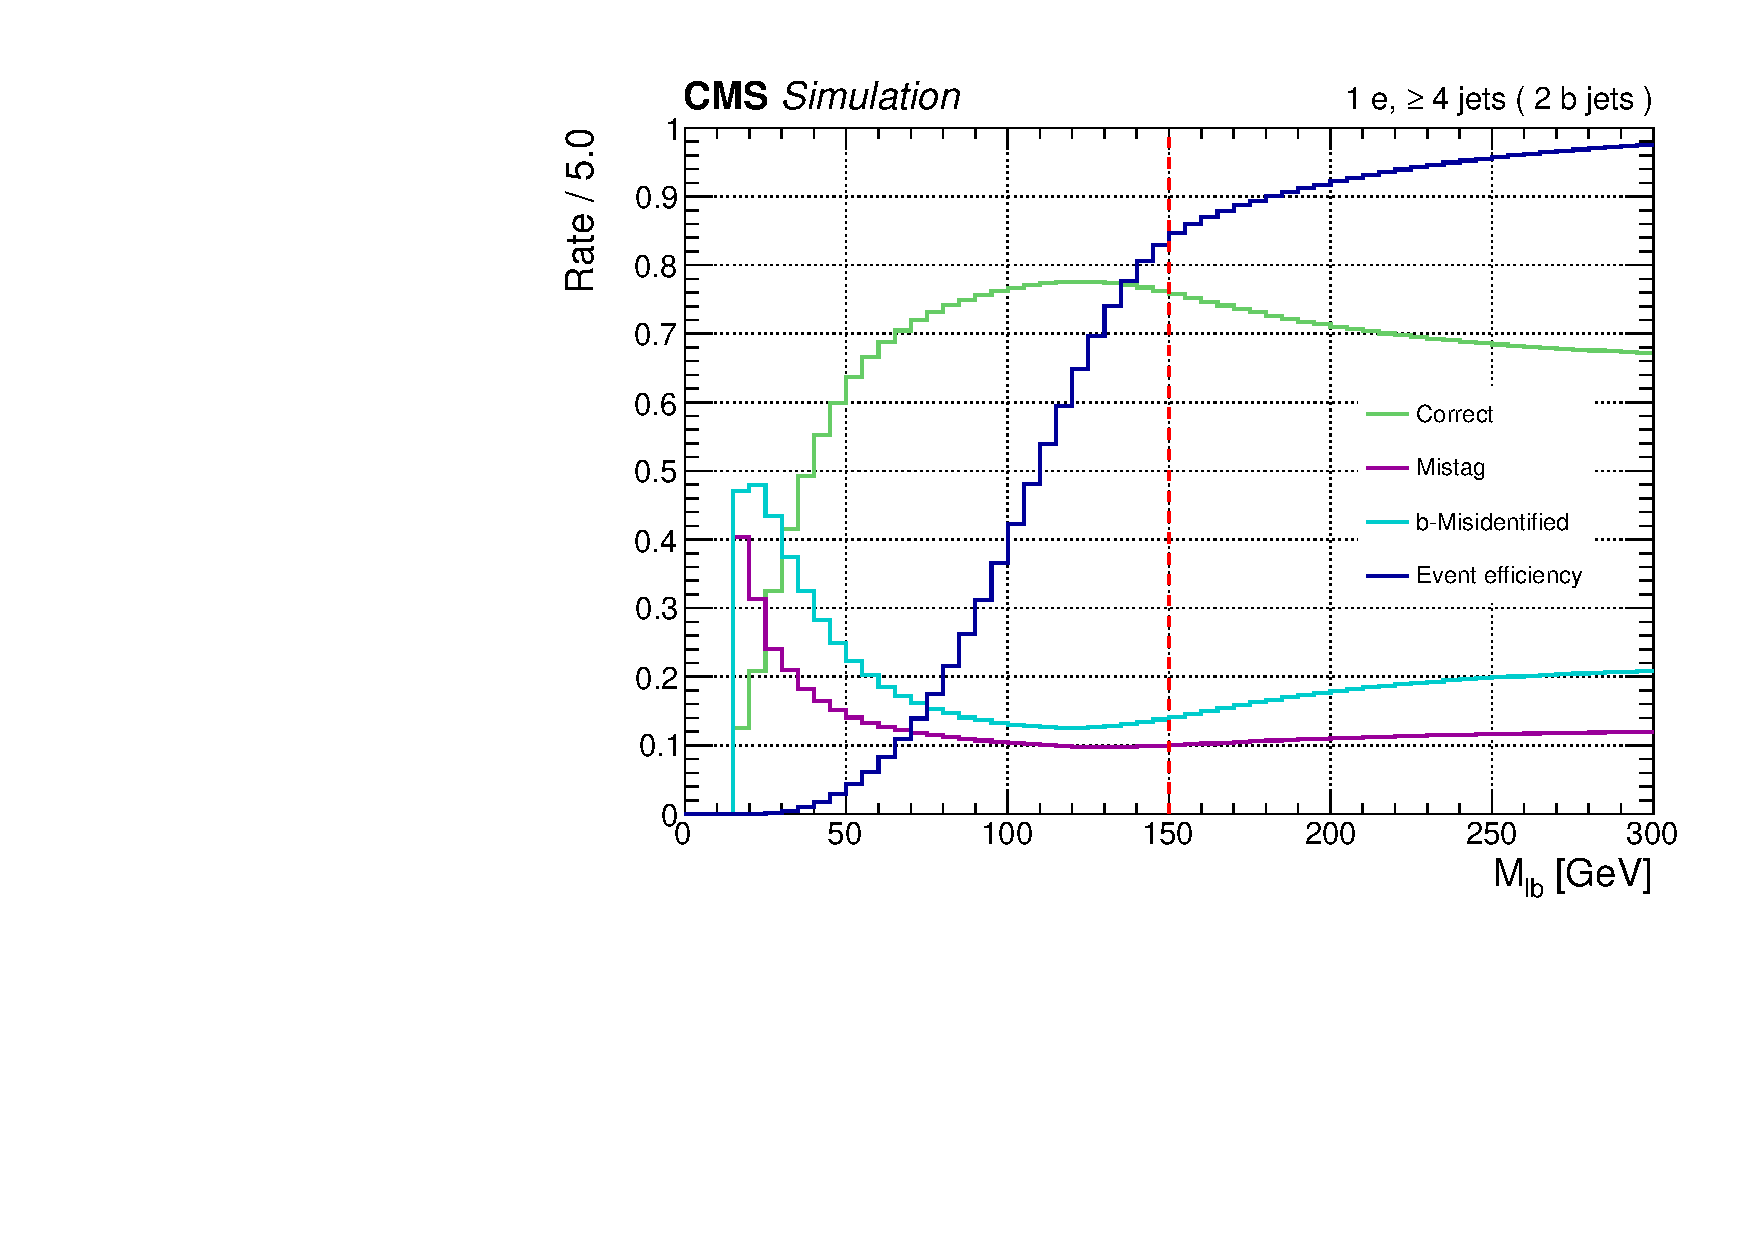
\includegraphics[width=0.45\textwidth]{figure/bbSep_18_el_OptCut_chi2_20_bbSep.pdf}
    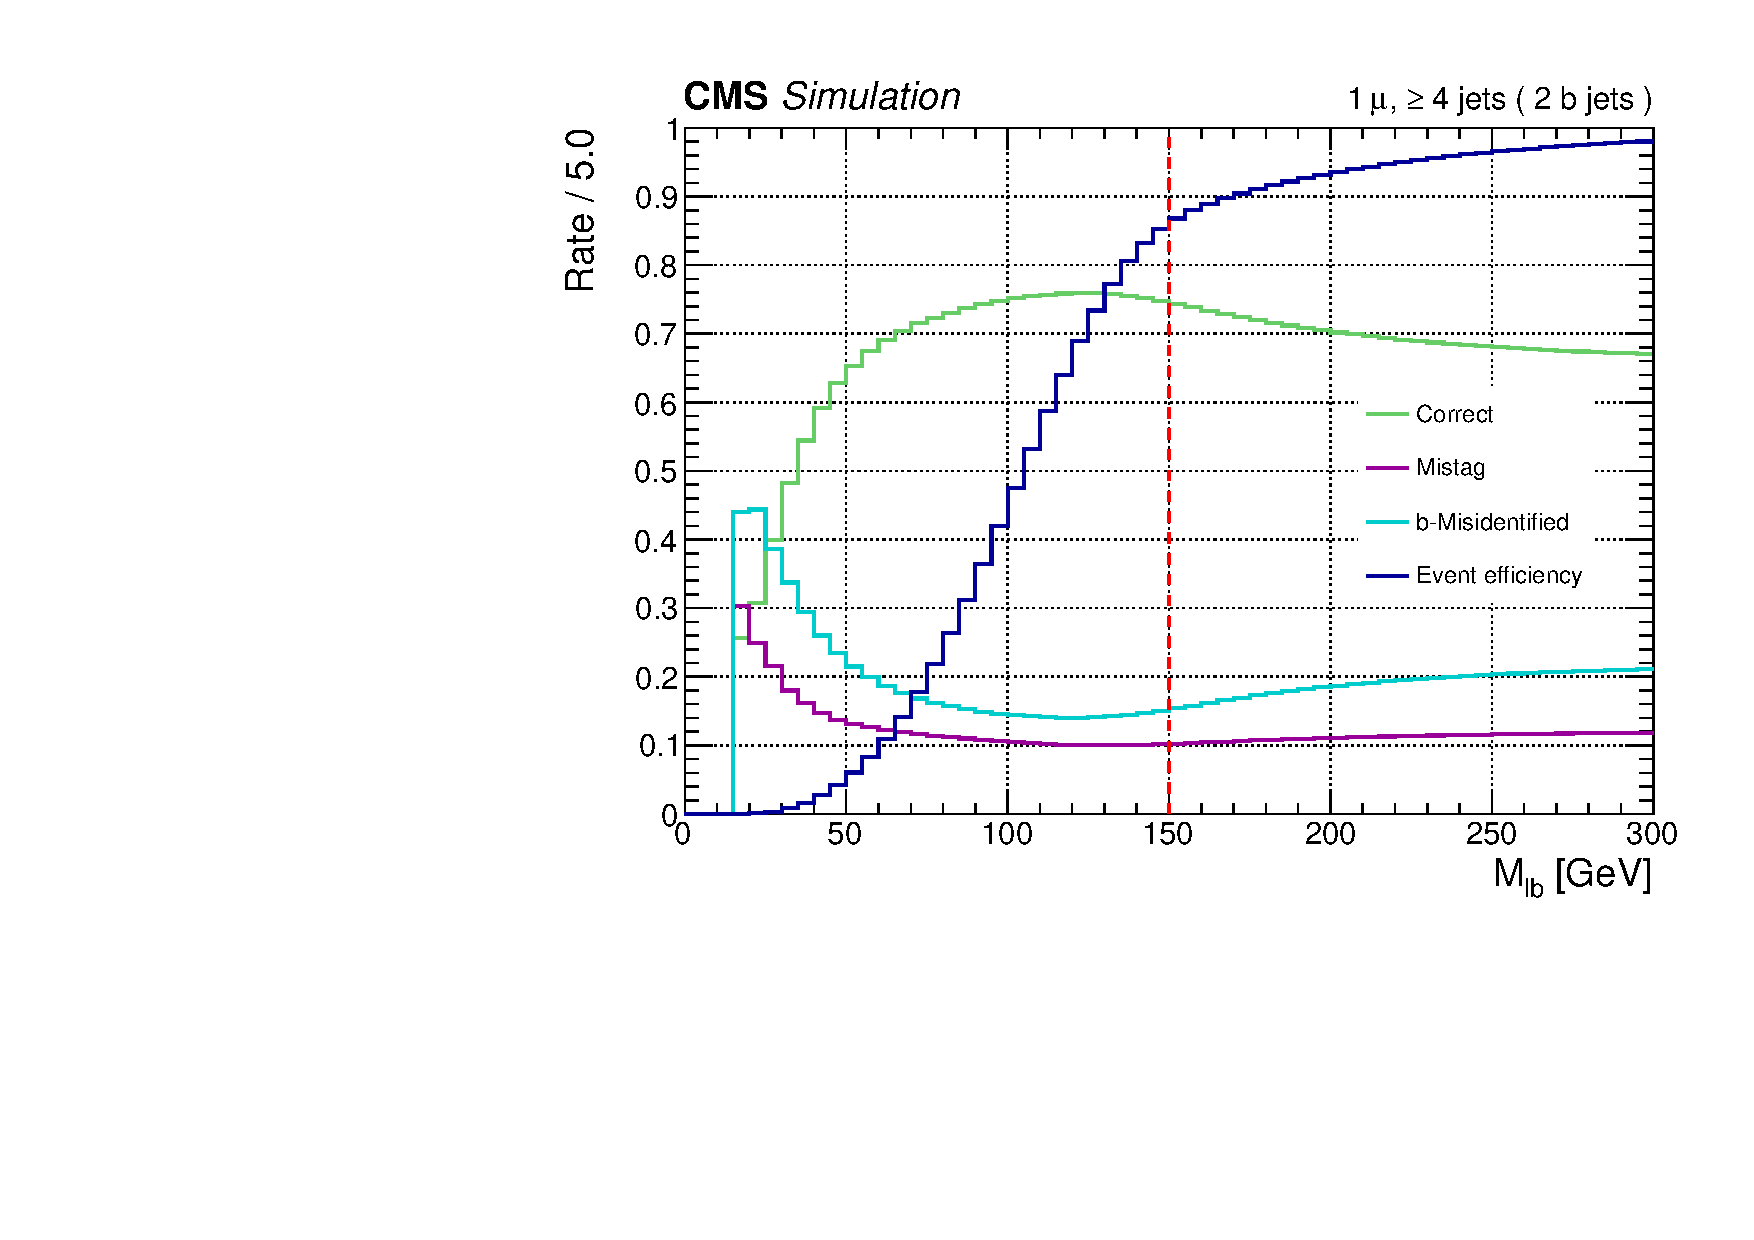
\includegraphics[width=0.45\textwidth]{figure/bbSep_18_mu_OptCut_chi2_20_bbSep.pdf}
    \caption[The fraction of each event type in \Mlb distribution.]
    {
        The fraction of each event type in \Mlb distribution with the event efficiency in electron channel (left) and muon channel (right) for 2016 (top), 2017 (middle), and 2018 (bottom) samples.
        The red dotted line shows the used uppeer bound in this analysis.
    }
    \label{fig:opt_cut}
\end{figure}

\begin{figure}
    \centering
    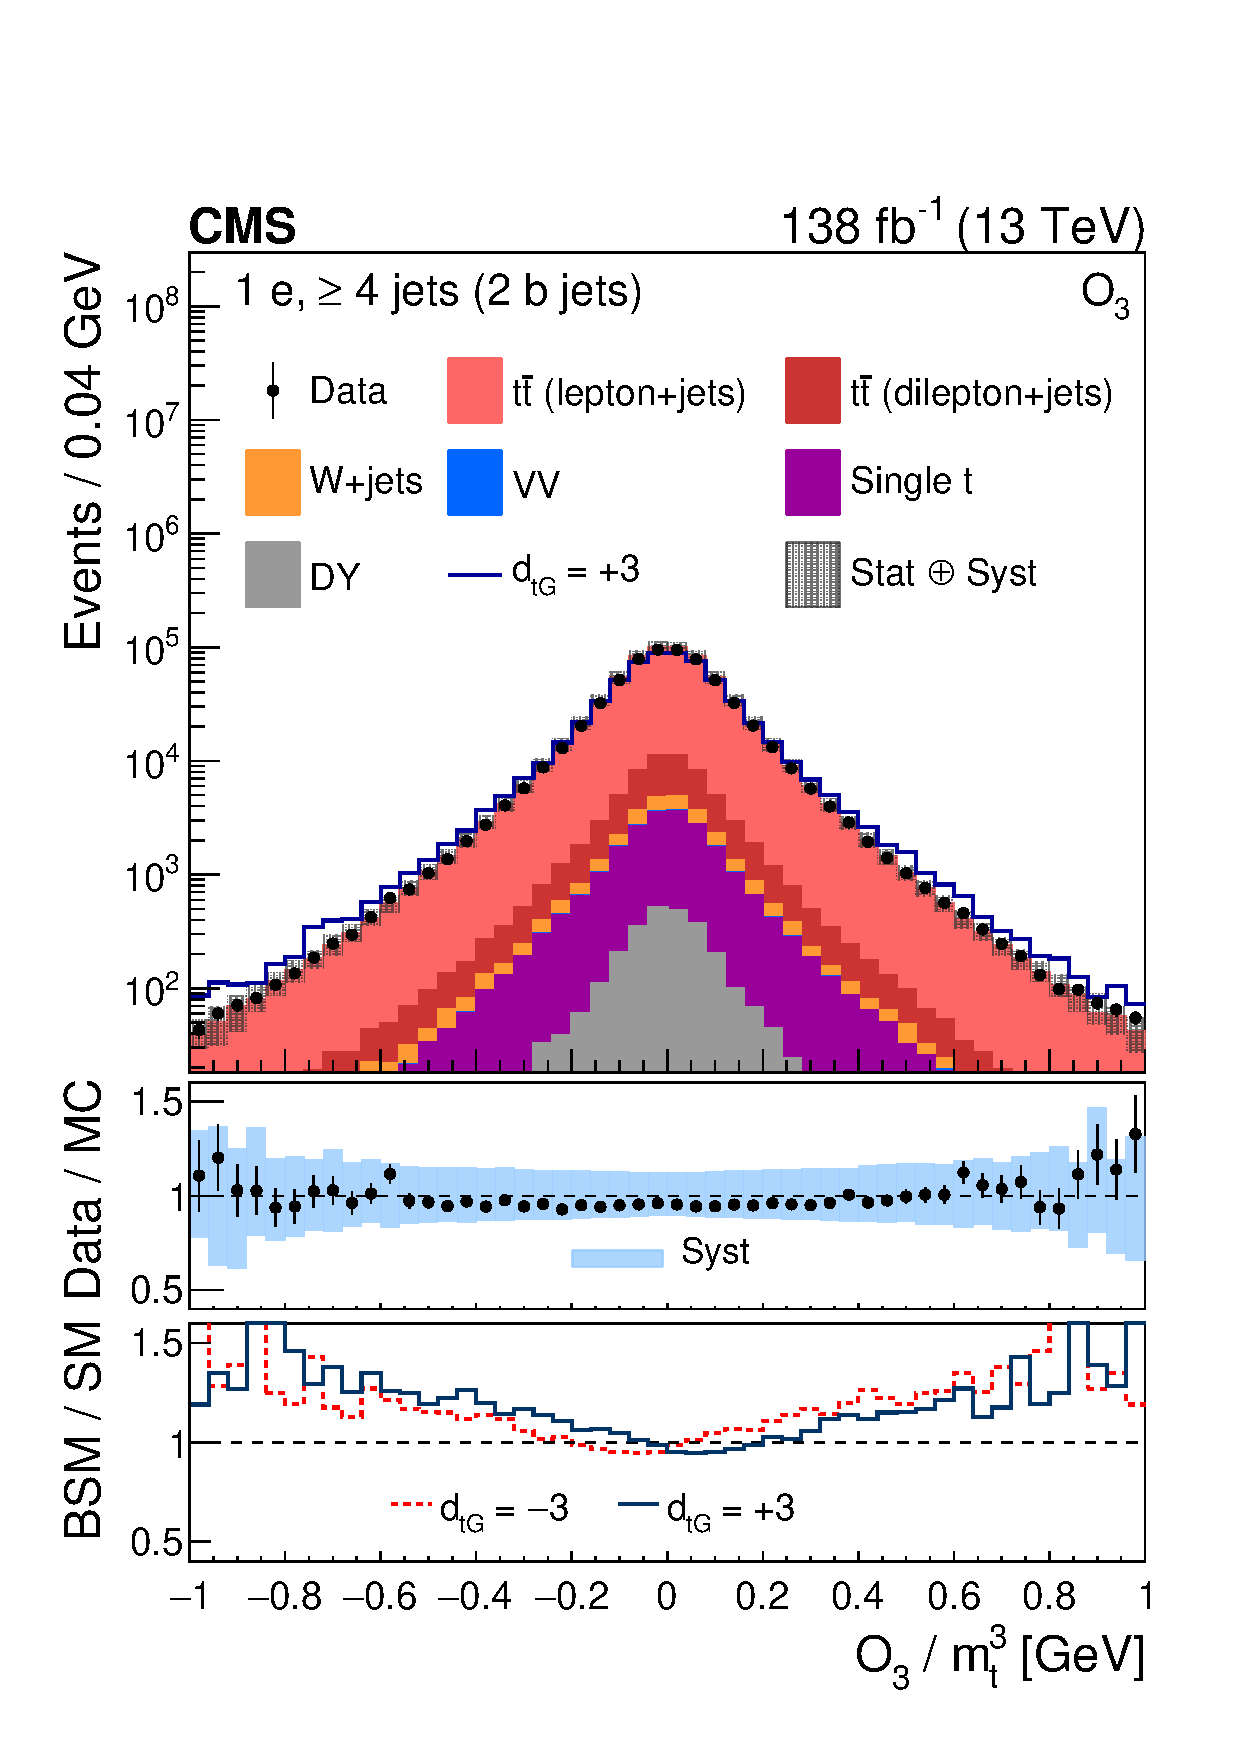
\includegraphics[width=0.4\textwidth]{figure/Figure_001-a.pdf}
    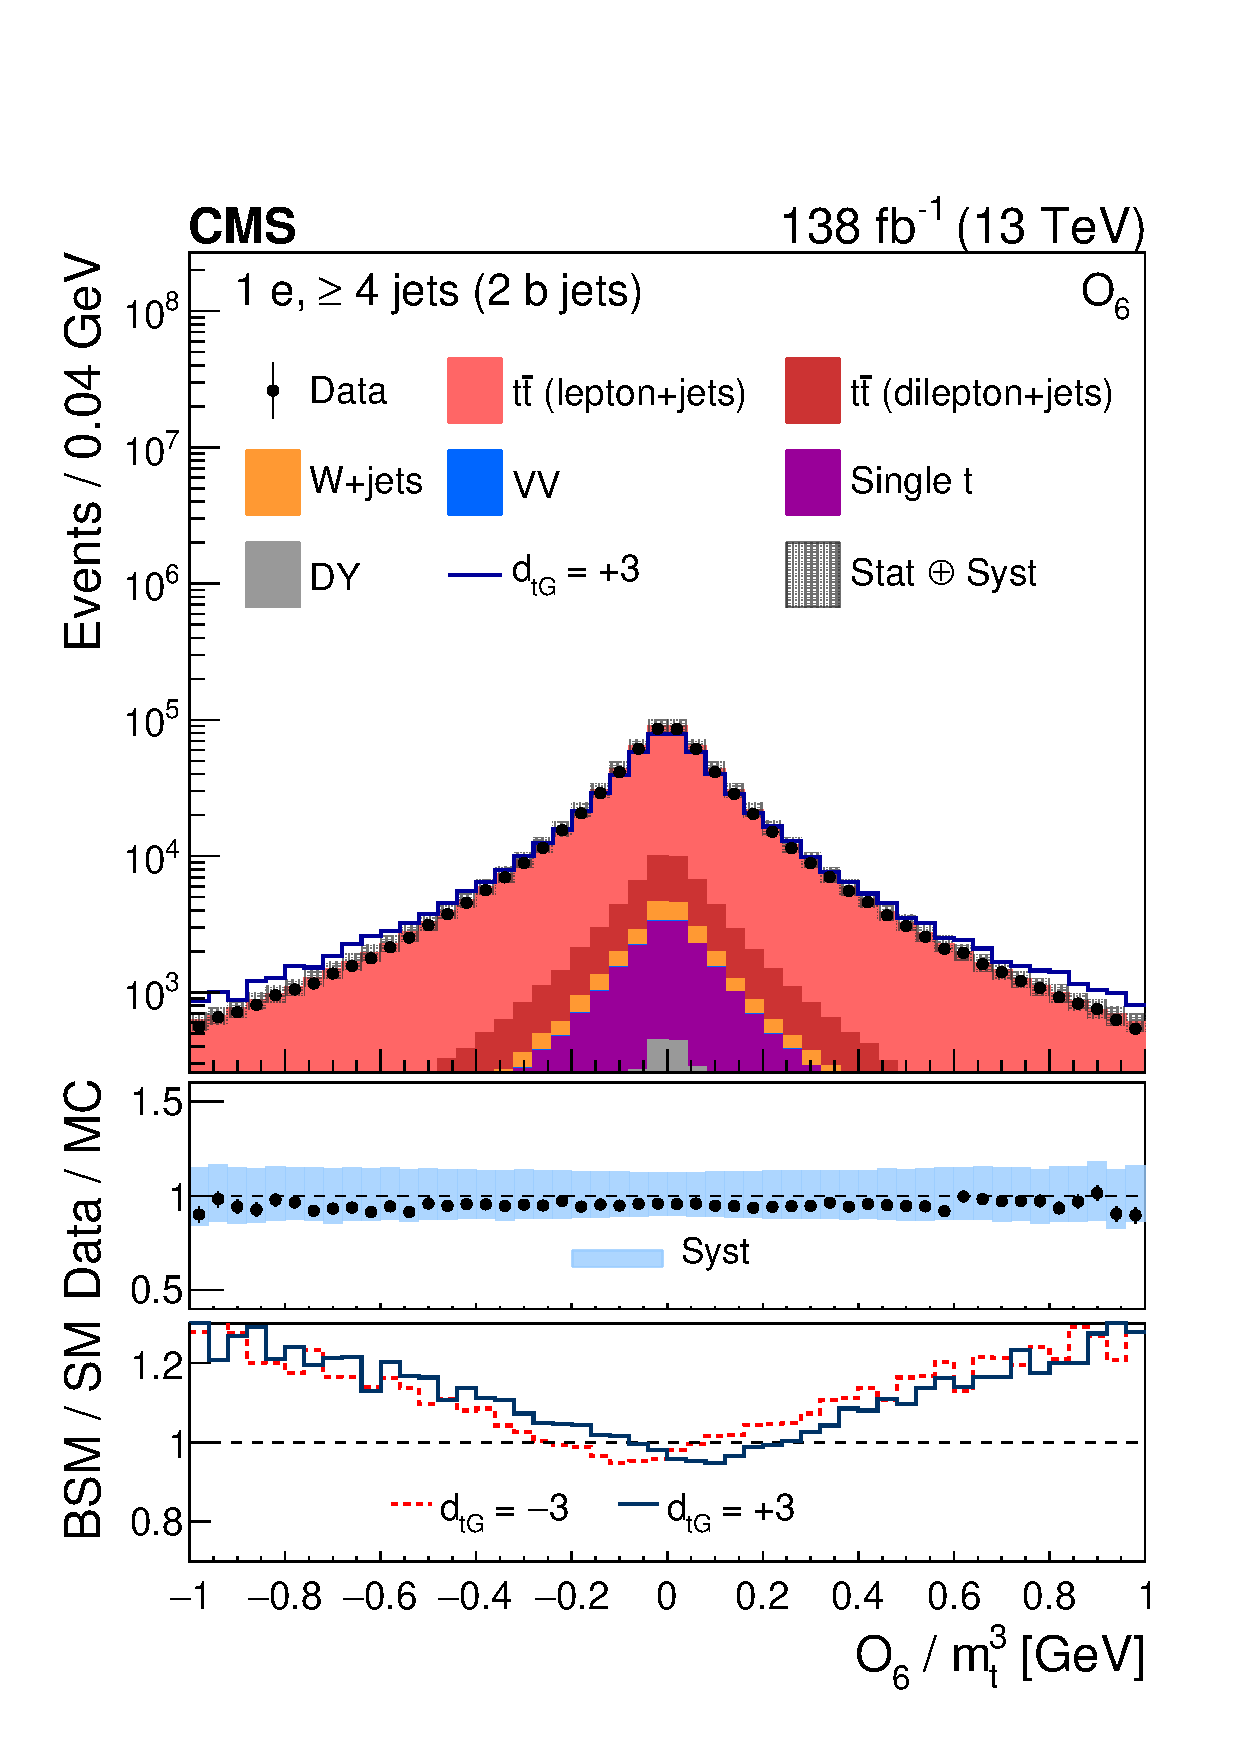
\includegraphics[width=0.4\textwidth]{figure/Figure_001-b.pdf}
    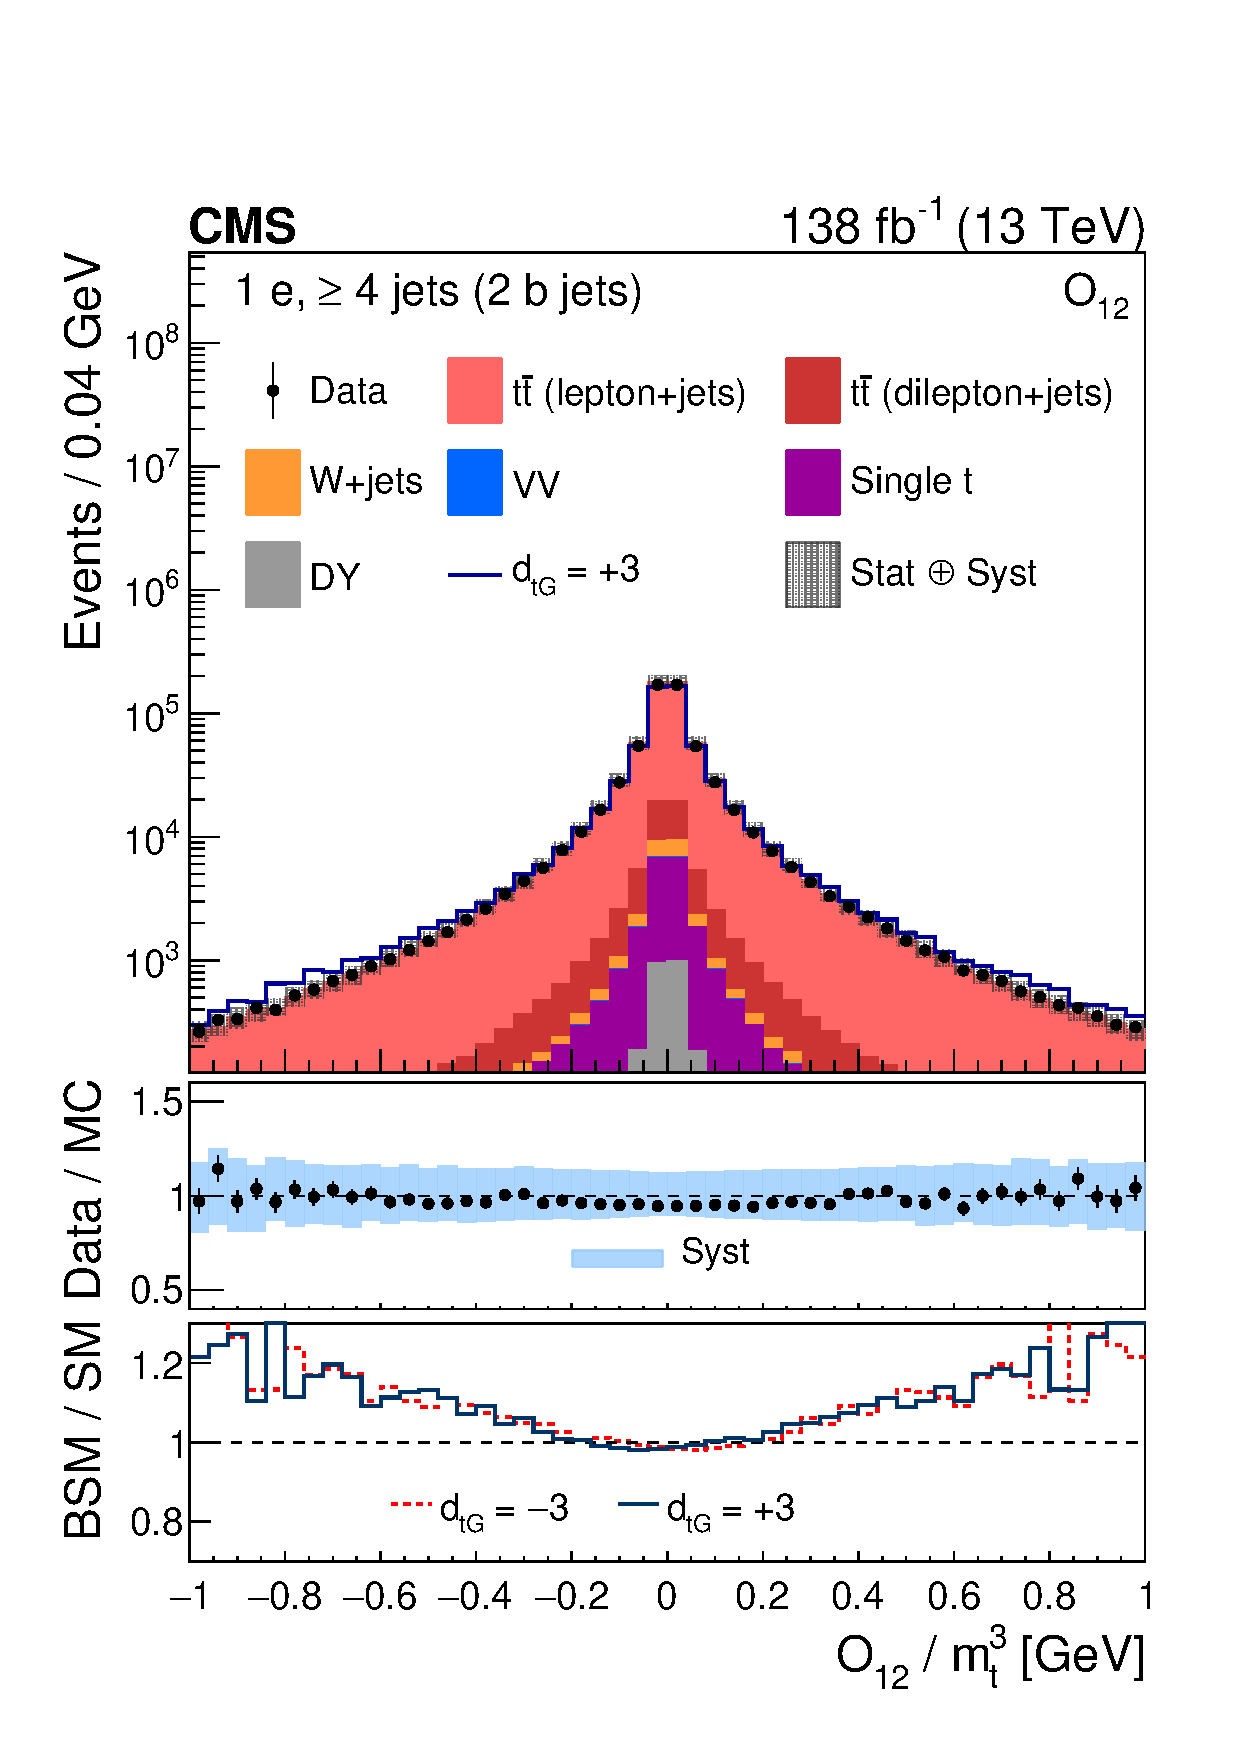
\includegraphics[width=0.4\textwidth]{figure/Figure_001-c.pdf}
    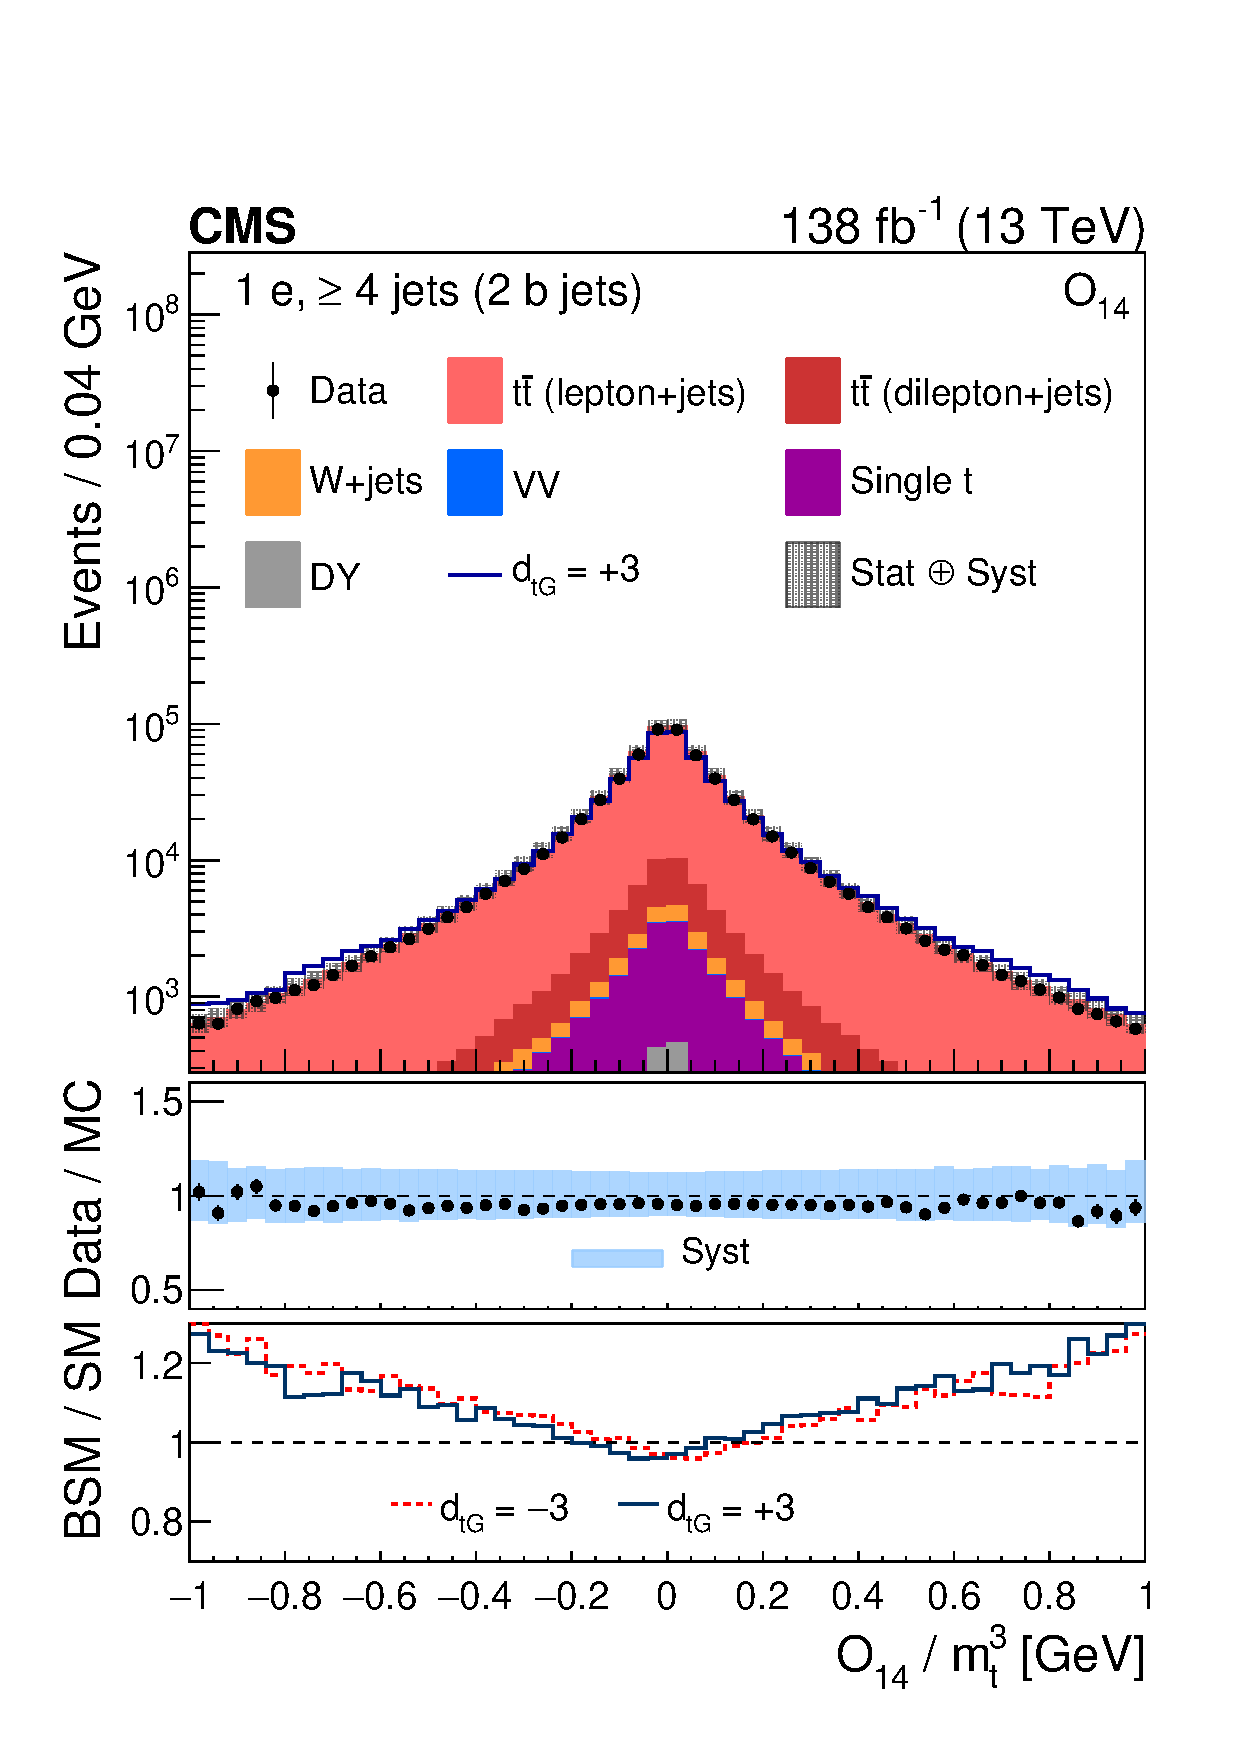
\includegraphics[width=0.4\textwidth]{figure/Figure_001-d.pdf}
    \caption[Distributions of the CP observables for electron events in the signal region.]
    {
        Distributions of the CP observables \Othree (upper left), \Osix (upper right), \Otwelve (lower left), and \Ofourteen (lower right), normalized with respect to \Mtcub, from data (points) and from the various sources in simulation (colored histograms) for electron events in the signal region.
        The solid-blue line shows the CEDM simulated signal normalized to the data with the CP-odd parameter $\dtG = +3$.
        The vertical bars on the data points indicate the statistical uncertainties in the data, and the hatched bands show the quadrature sum of the statistical and systematic uncertainties in the simulation.
        The lower two panels display the ratio of the data to the sum of the MC predictions and the ratio of the CEDM to the SM predictions for $\dtG = +3$ (dark-blue lines) and $-3$ (red lines).
    }
    \label{fig:el_obs_dist}
\end{figure}

\begin{figure}
    \centering
    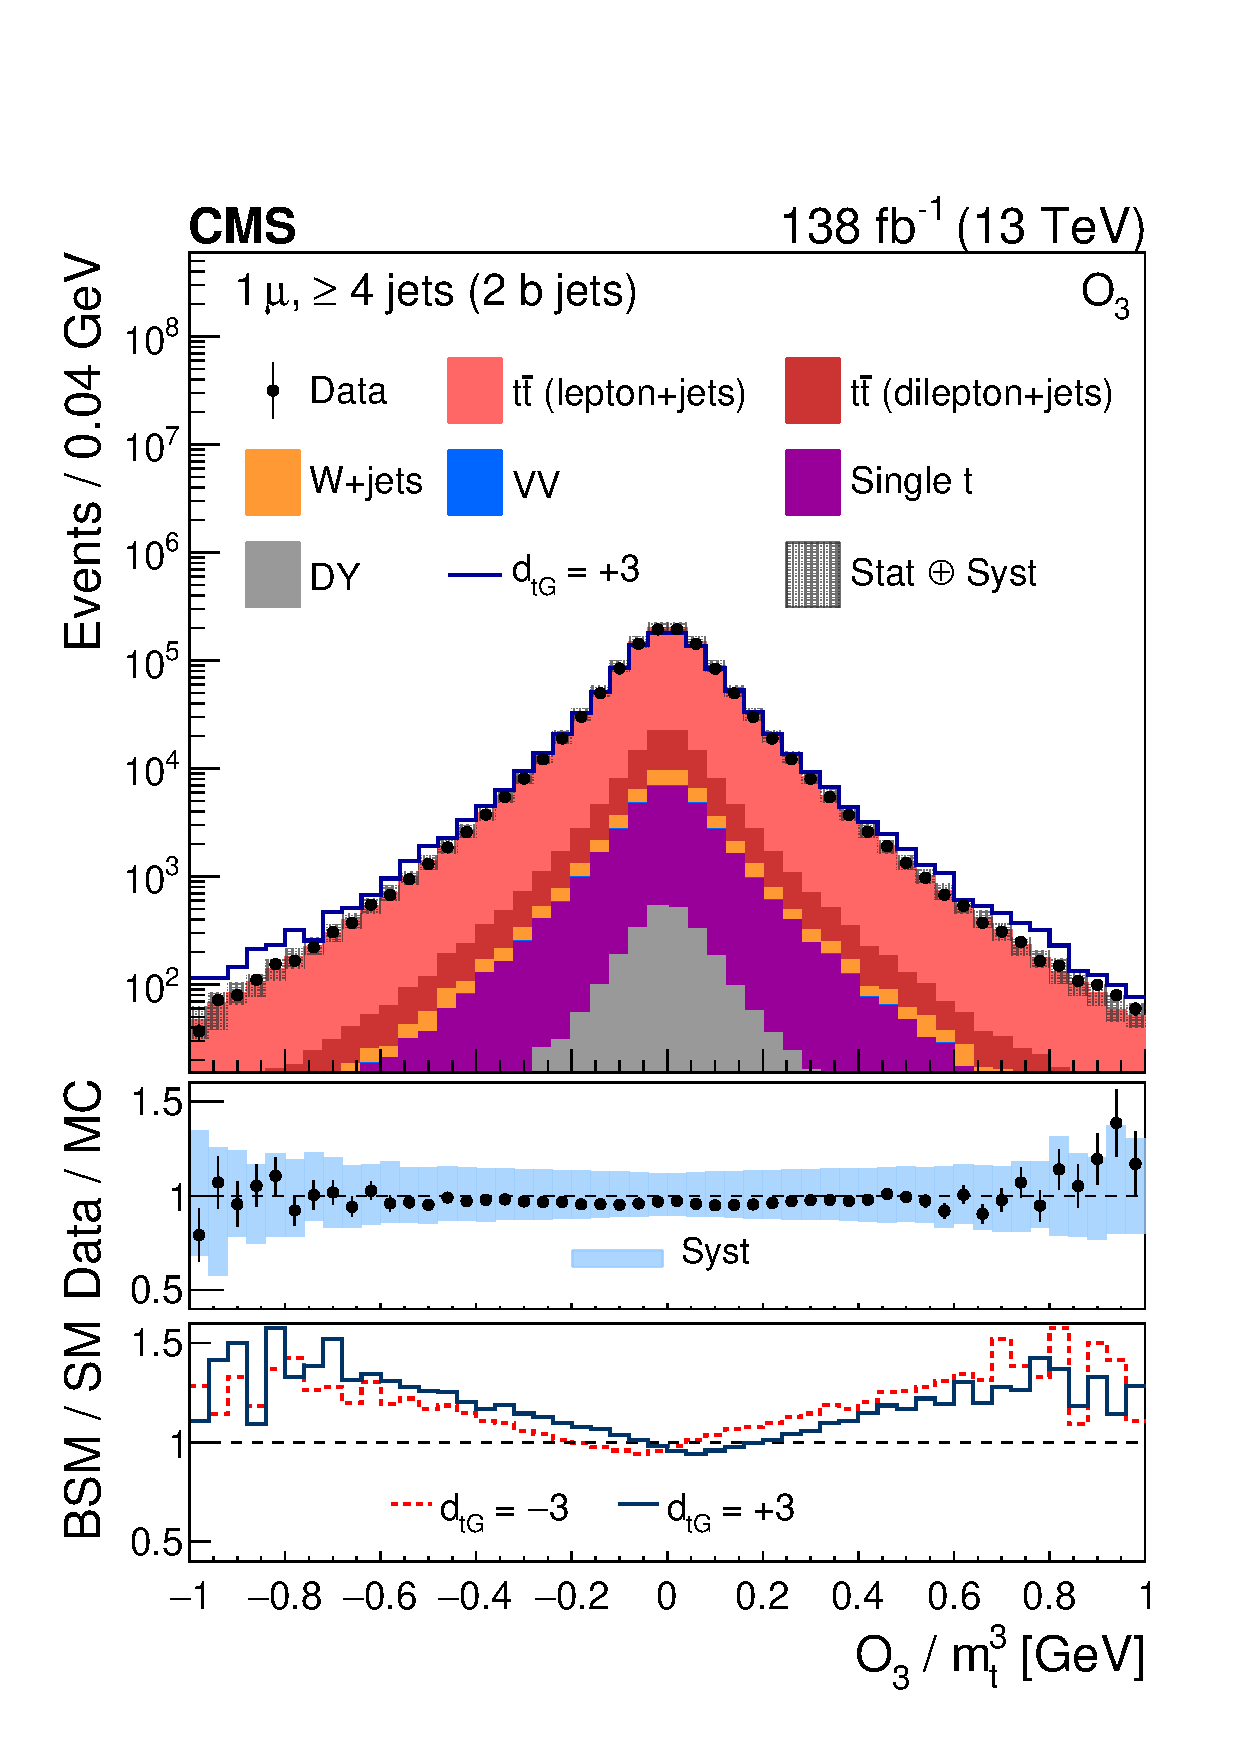
\includegraphics[width=0.4\textwidth]{figure/Figure_002-a.pdf}
    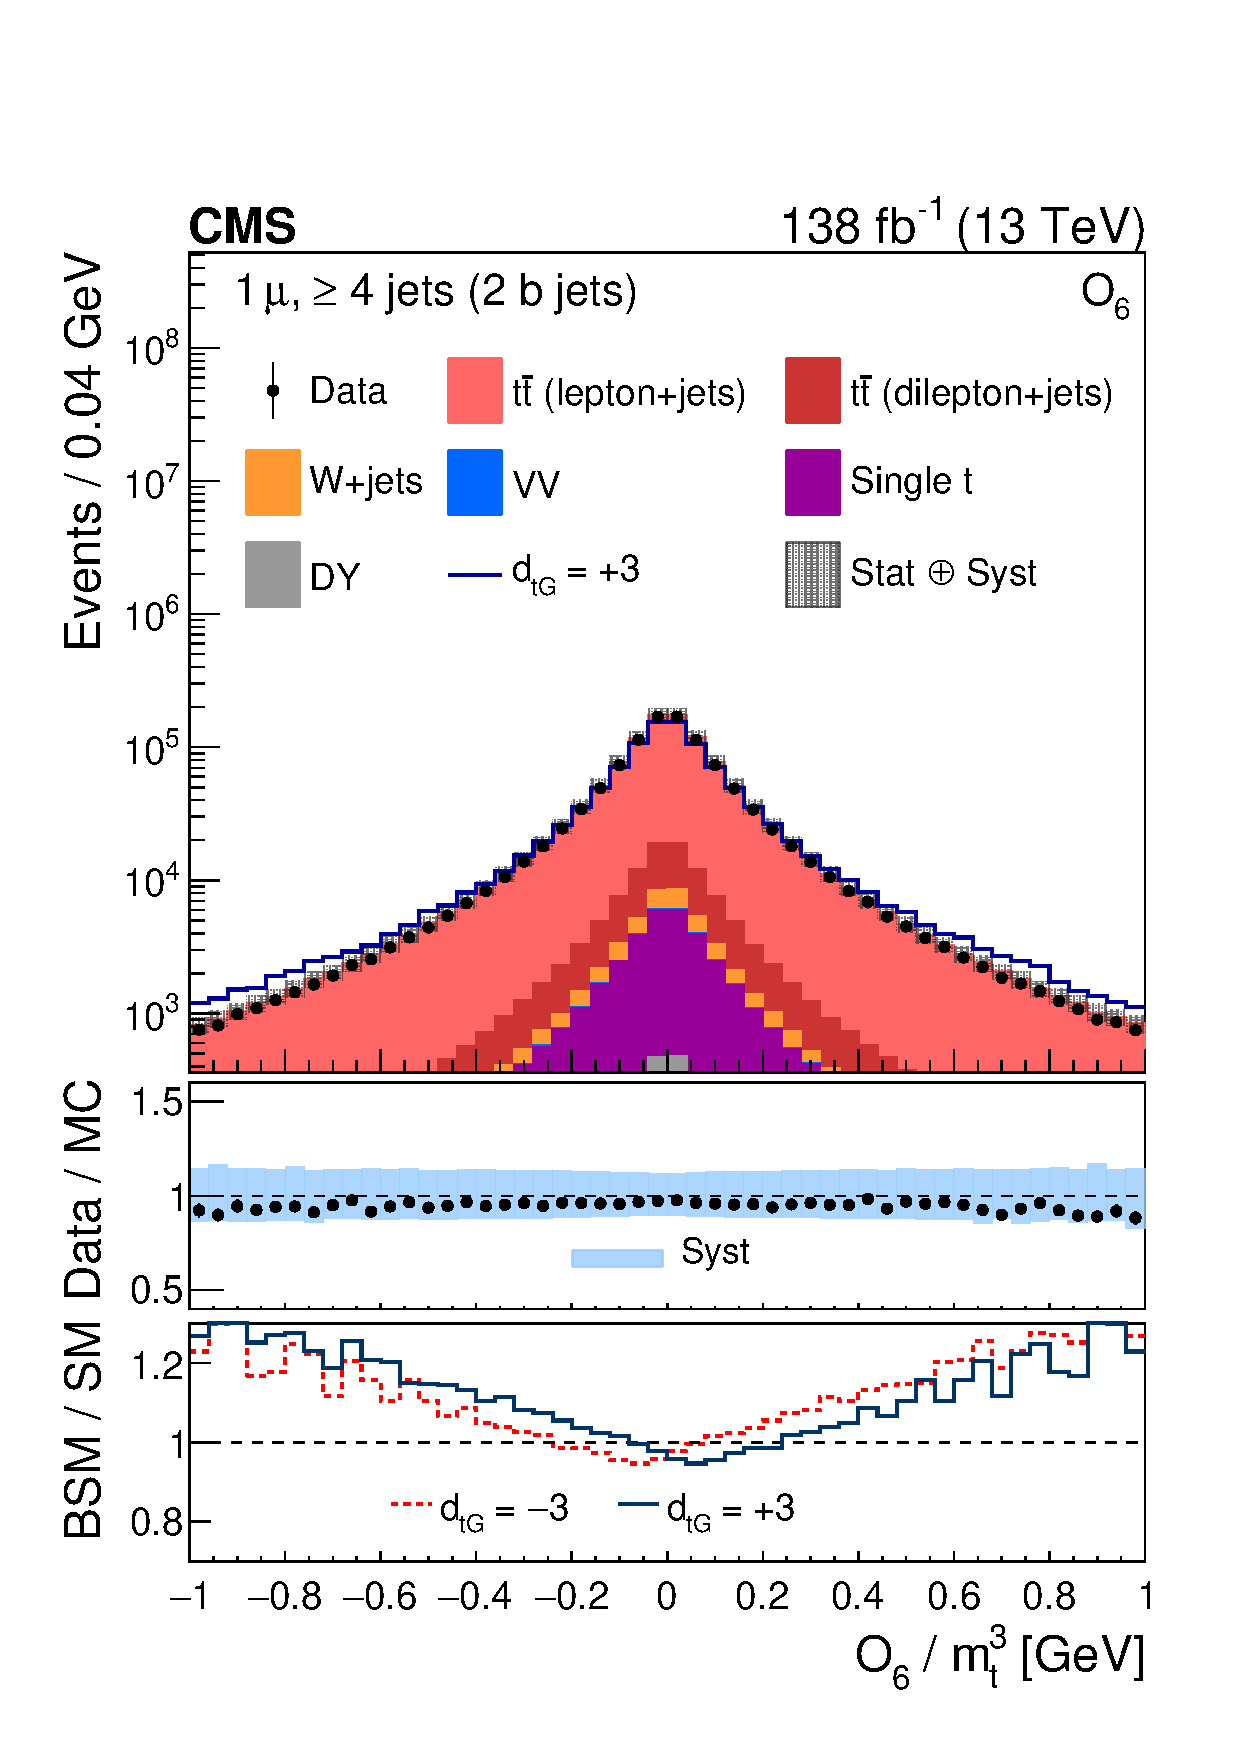
\includegraphics[width=0.4\textwidth]{figure/Figure_002-b.pdf}
    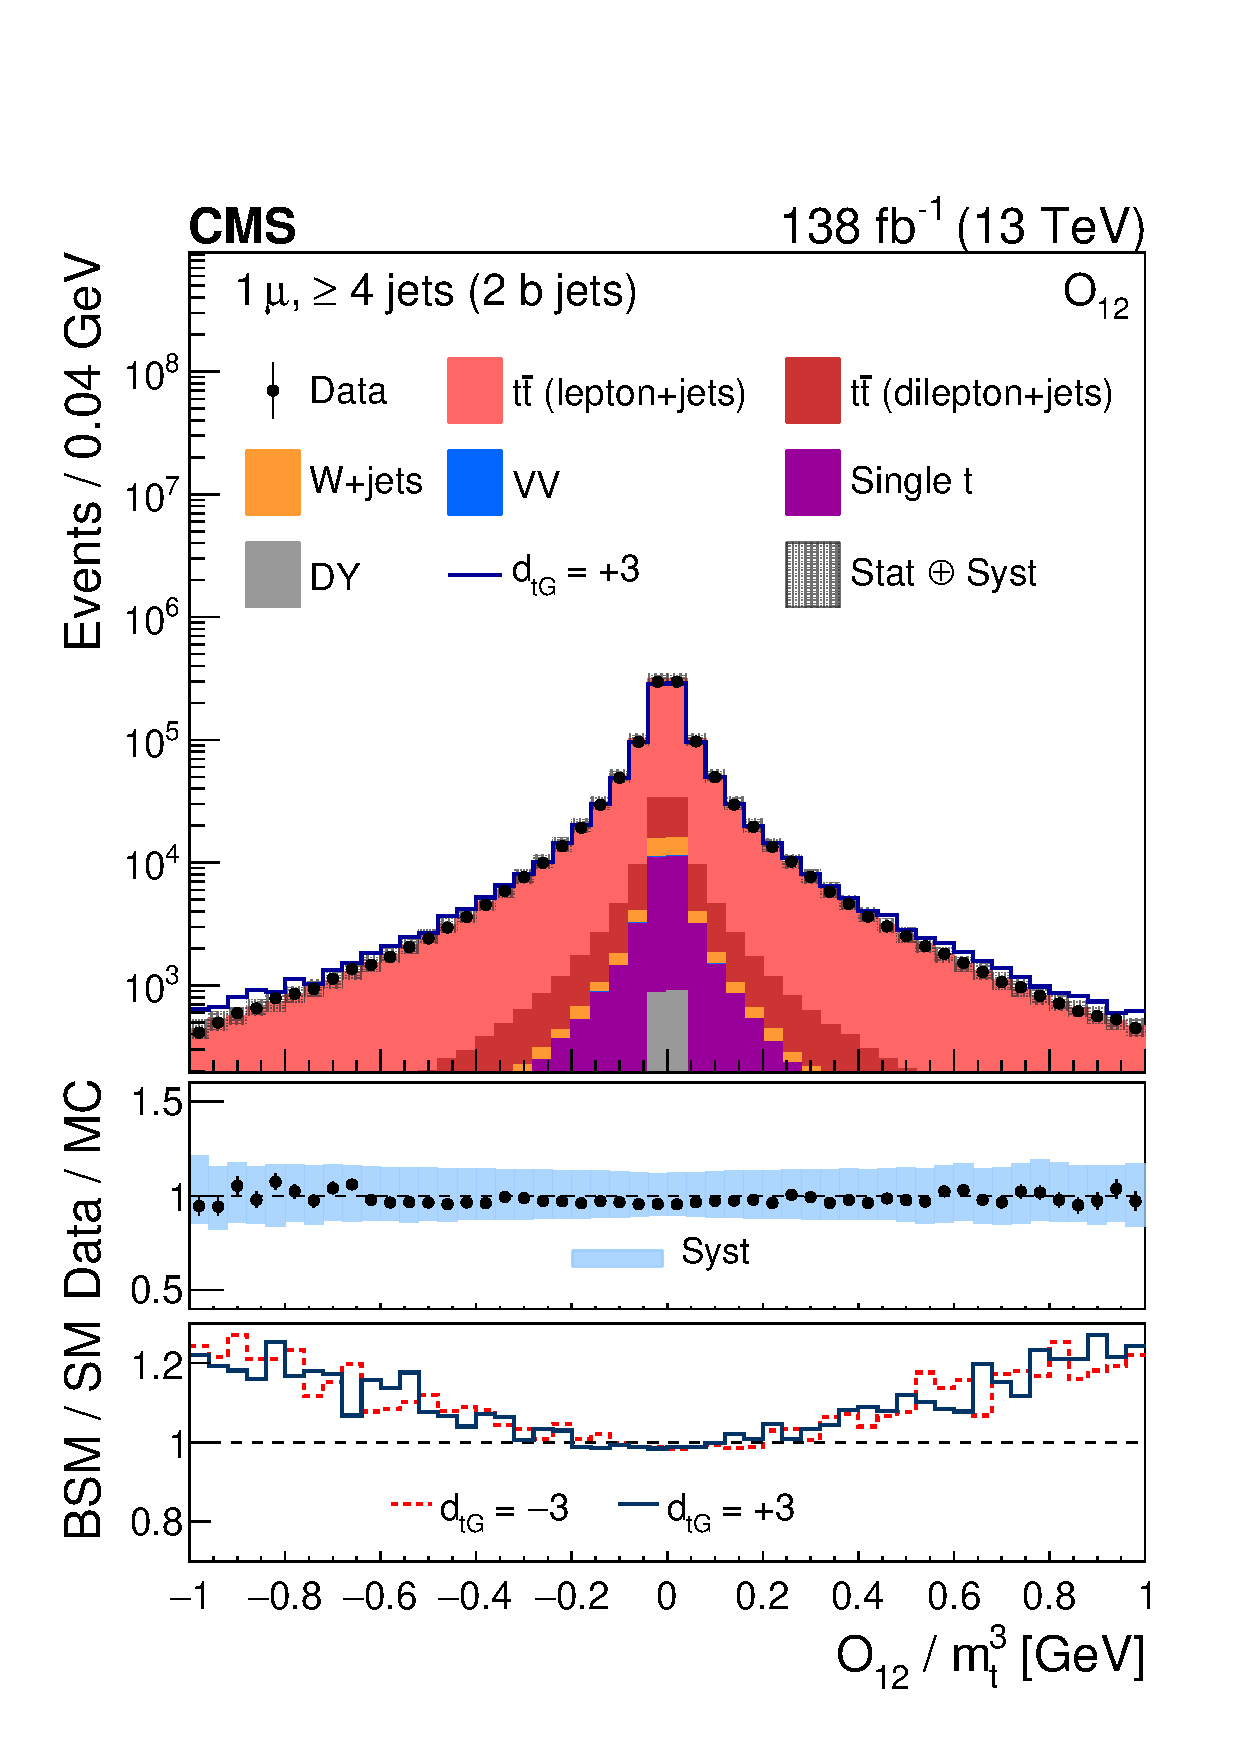
\includegraphics[width=0.4\textwidth]{figure/Figure_002-c.pdf}
    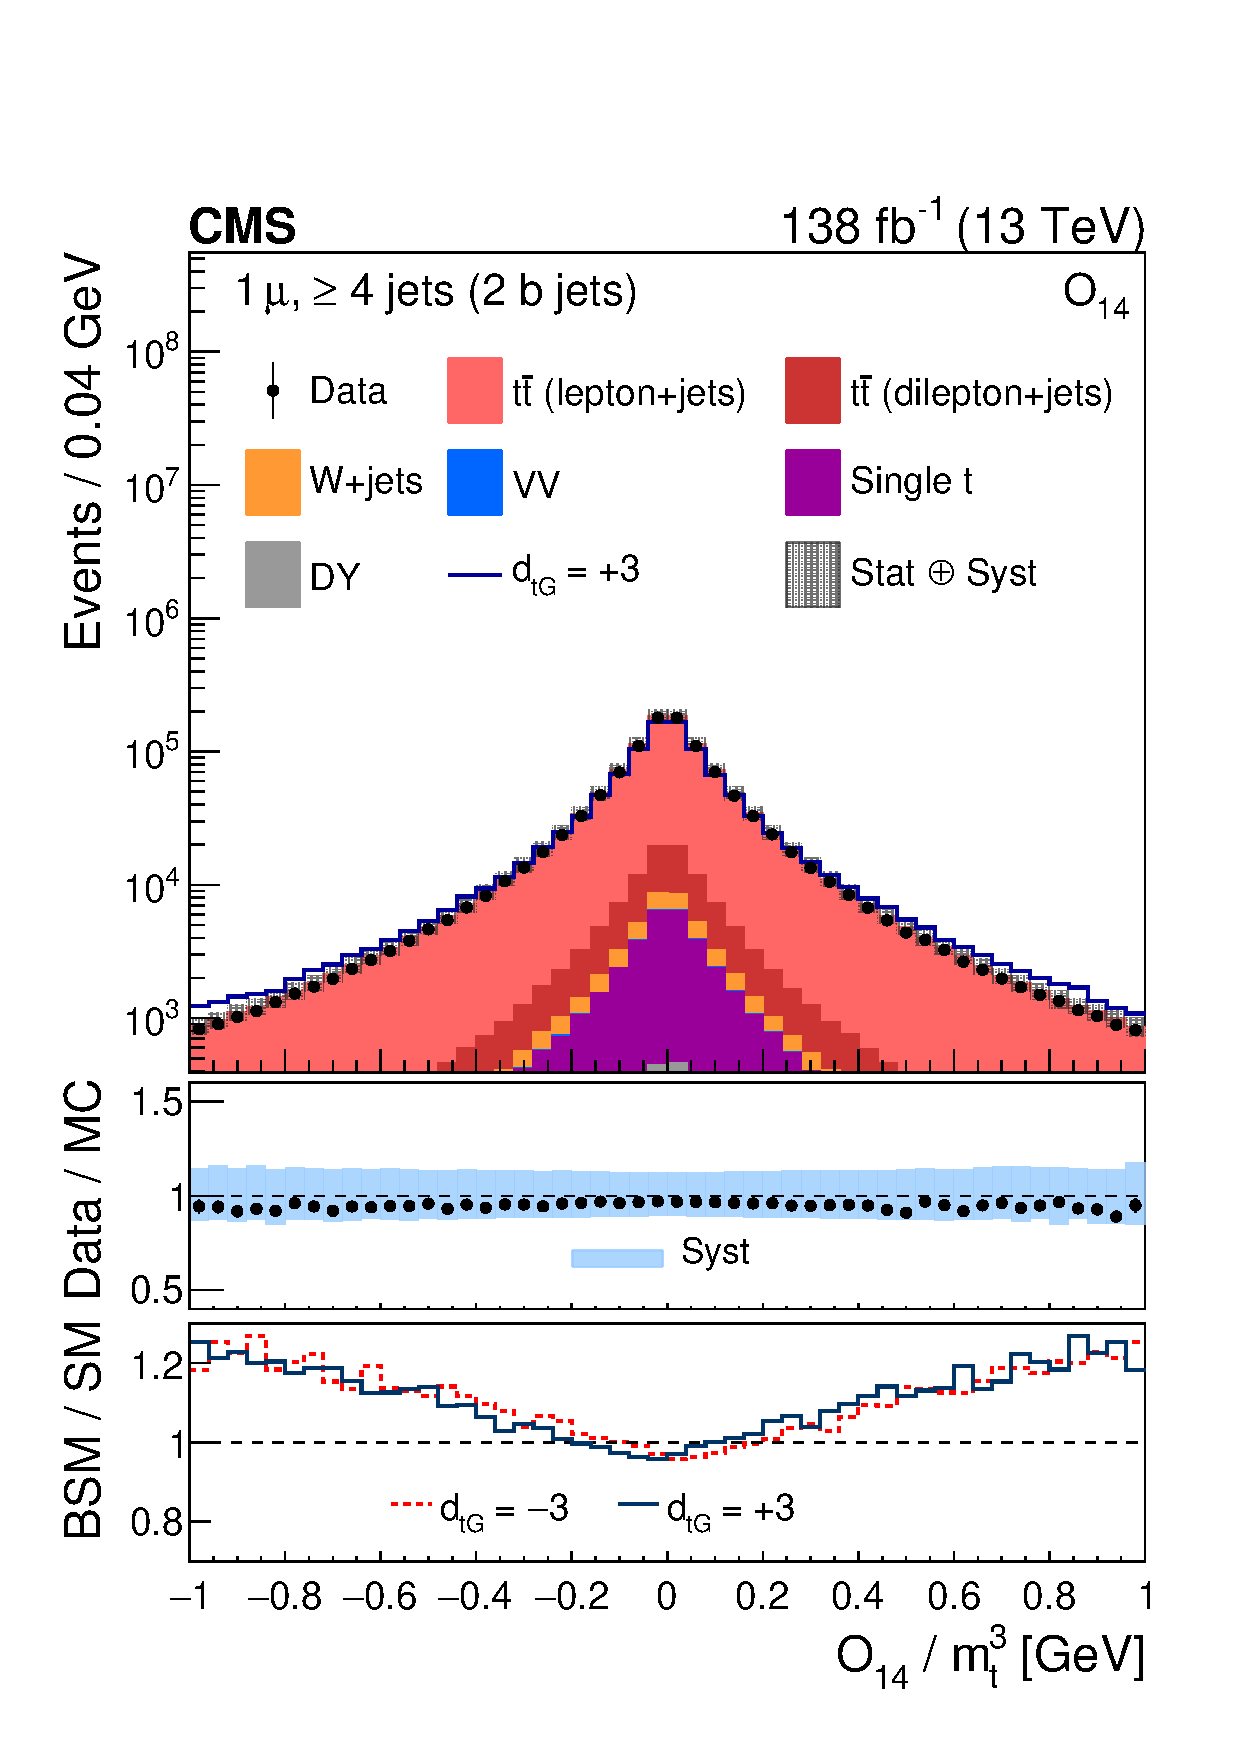
\includegraphics[width=0.4\textwidth]{figure/Figure_002-d.pdf}
    \caption[Distributions of the CP observables for muon events in the signal region.]
    {
        Distributions of the CP observables \Othree (upper left), \Osix (upper right), \Otwelve (lower left), and \Ofourteen (lower right), normalized with respect to \Mtcub, from data (points) and from the various sources in simulation (colored histograms) for muon events in the signal region.
        The solid-blue line shows the CEDM simulated signal normalized to the data with the CP-odd parameter $\dtG = +3$.
        The vertical bars on the data points indicate the statistical uncertainties in the data, and the hatched bands show the quadrature sum of the statistical and systematic uncertainties in the simulation.
        The lower two panels display the ratio of the data to the sum of the MC predictions and the ratio of the CEDM to the SM predictions for $\dtG = +3$ (dark-blue lines) and $-3$ (red lines).
    }
    \label{fig:mu_obs_dist}
\end{figure}

\begin{table}
    \caption[The predicted \ttbar signal and background contributions to the signal events.]
    {
        The predicted \ttbar signal and background contributions to the signal events from simulation for the electron and muon channels.
    }
    \label{tab:signal_region_expected_percentage}
    \centering\renewcommand\arraystretch{1.2}
    \begin{tabular}{ccc}
        Process & Electron channel (\%) & Muon channel (\%) \\
        \hline
        \ttbar in lepton+jets & 89.9 & 89.5\\
        \ttbar in dilepton+jets & 5.5 & 5.5\\
        \ttbar multijet & 0.1 & 0.1\\
        Single \PQt & 2.9 & 2.9\\
        \Wjets & 1.0 & 1.1\\
        DY+jets & 0.4 & 0.2\\
        QCD multijet & 0.2 & 0.6\\
        $\PZ\PZ$ / $\PW\PW$ / $\PW\PZ$ & 0.1 & 0.1\\
    \end{tabular}
\end{table}

Background events can induce spurious measurements of the asymmetries, so a sample of background-enriched data events is used to check for such effects.
In order to enhance the fraction of background events and minimize the contribution from \ttbar, events are required to have no \PQb-tagged jets.
The \PQb jet veto is defined using a weakly restrictive working point of \DeepCSV, corresponding to an 84\% efficiency in identifying \PQb jets and an 11\% misidentification rate for light-flavor quark and gluon jets~\cite{CMS:bjet_eff}.
The isolation requirement in the looser set of selection criteria for leptons is relaxed, so events with additional leptons produced through the decay of a bottom quark can be more highly rejected.
The rest of the selection criteria are the same as used for the signal events.
The object assigned by the $\chisq$ algorithm takes the role of the \PQb jet coming from the hadronically decaying top quark, and the jet closest to the isolated lepton is assigned as the other \PQb jet.
The background-enriched events are expected to be dominated by non-\ttbar processes ($\approx$90\%), including a major contribution from \Wjets.
